\chapter{Selección de eventos y optimización de las regiones de señal}
\label{ch:evt_selection}
\epigraph{\emph{``I don't want to believe. I want to know.”}}{Carl Sagan}

El estado final fotón+jet en la región de alta masa invariante representa un escenario ideal para búsquedas de física \ac{BSM}, pero para ello es imprescindible tener un excelente conocimiento del fondo producido por los procesos del \ac{SM}.

En las búsquedas de resonancias es habitual diseñar regiones de señal que sean capaces de proporcionar un fondo suave pero también una señal limpia sobre él. En este capítulo se presenta la selección de eventos que conduce a las regiones de señal utilizadas en este análisis.


\section{Trigger}
\label{sec:evt_selection:trigger}

Los eventos se recogen mediante un trigger de un sólo fotón (\texttt{HLT\_g140\_loose}) con un umbral de momento transverso de \(140~\gev\), que es el trigger de fotón sin preescalar de más bajo \pt para la mayor parte de los periodos de toma de datos\footnote{Para el año 2015, el trigger de más bajo \pt sin preescalar fue el \texttt{HLT\_g120\_loose}, pero el \texttt{HLT\_g140\_loose} también estaba en el menú}, seleccionando eventos con al menos un fotón que pasa el criterio de identificación \texttt{Loose}. Este trigger se ha mantenido sin escalar y es totalmente eficiente para fotones con \(>145~\gev\) con incertezas menores de \(0.1\%\) por encima de \(150~\gev\). Esta eficiencia se ha calculado con un método bootstrap siguiendo las prescripciones de la \Refn{\cite{ATLAS-PhotonTrigger-Performance-2015}} y se muestra en la \Fig{\ref{fig:evt_selection:trigger:trigger_perf_15_18}} en función de \(\ptgam\), \(\etagam\) y \(\avgmu\) para los diferentes años de toma de datos.

\begin{figure}[ht!]
    \centering
    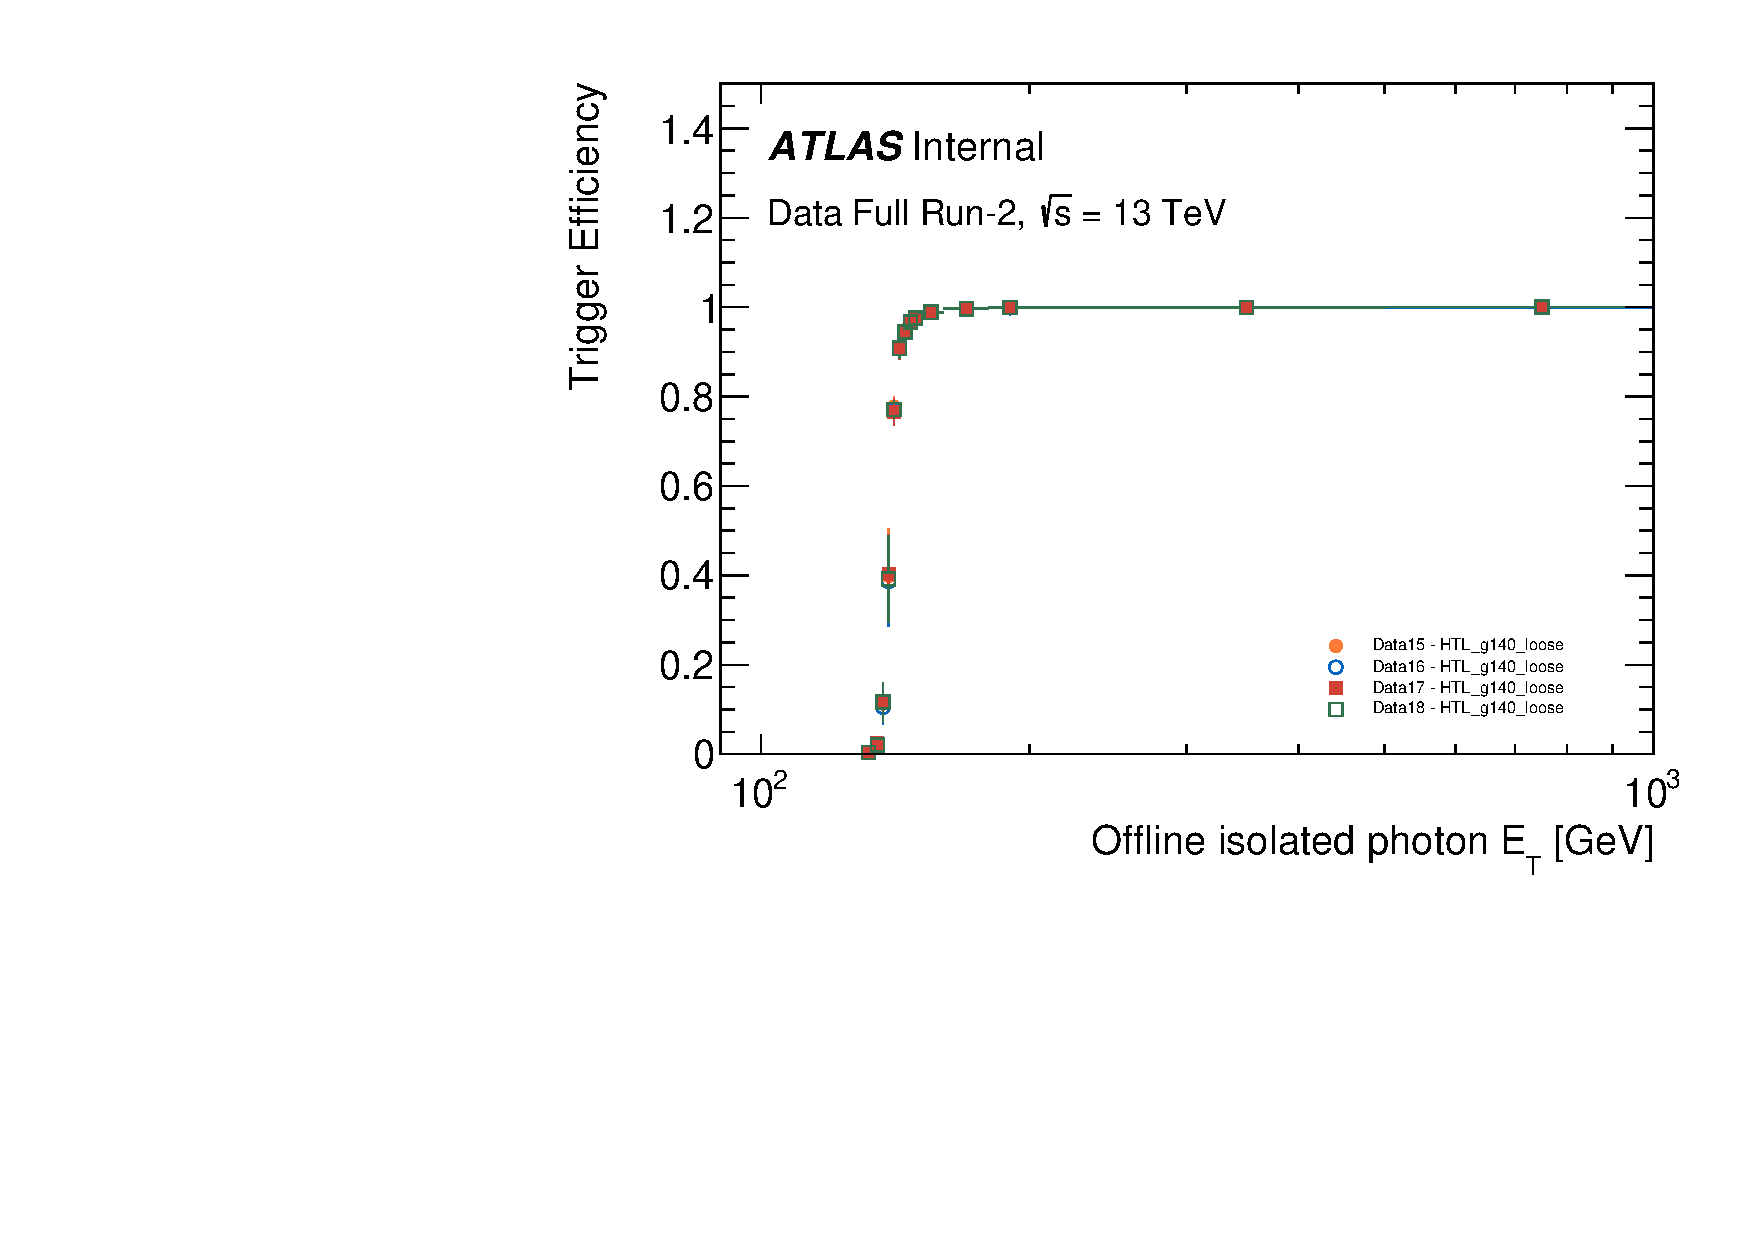
\includegraphics[width=0.32\textwidth]{5_resonances/event_selection/trigger/perfPlots_2015-2018_thesis_DATA_Et_g140_loose}
    \includegraphics[width=0.32\textwidth]{5_resonances/event_selection/trigger/perfPlots_2015-2018_thesis_DATA_eta_g140_loose}
    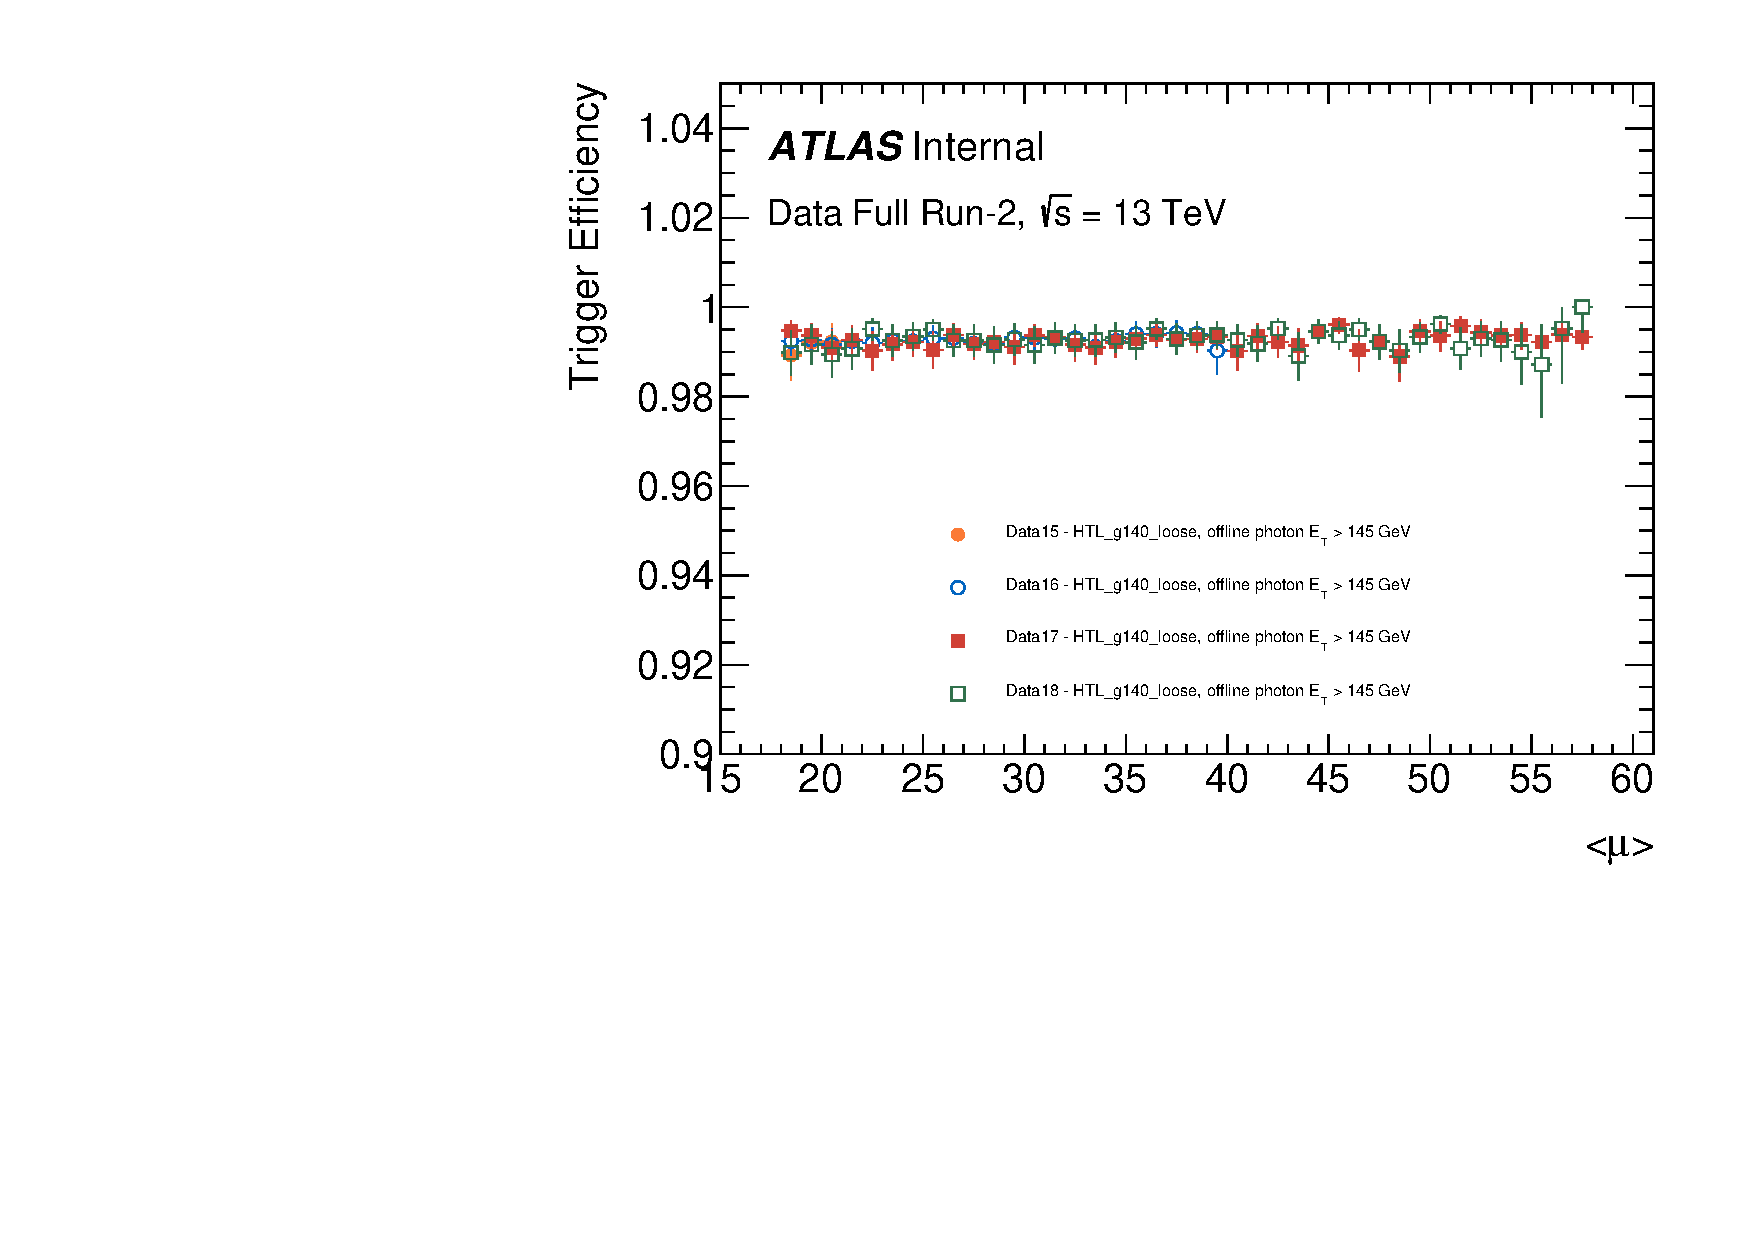
\includegraphics[width=0.32\textwidth]{5_resonances/event_selection/trigger/perfPlots_2015-2018_thesis_DATA_avmu_g140_loose}
    \caption{Eficiencia del trigger \texttt{HLT\_g140\_loose} en función de \(\ptgam\) (izquierda), \(\etagam\) (centro) y \(\avgmu\) (derecha) medida utilizando datos de cada año entre 2015 y 2018.}
    \label{fig:evt_selection:trigger:trigger_perf_15_18}
\end{figure}








\section{Preselección}
\label{sec:evt_selection:presel}



Como se discute en la \Sect{\ref{sec:atlas:runs}}, durante un período de toma de datos, los eventos recolectados por el detector \ac{ATLAS} se agrupan en \acp{LB} para luego compilarlos en \acp{GRL}. Estas \acp{GRL} garantizan que los datos utilizados están libres de ineficiencias del detector o subdetectores, o en el haz del \ac{LHC}. Este análisis utiliza el conjunto completo de datos del Run-2 recolectados durante los años 2015 a 2018 a una energía de centro de masa de \(\sqs = 13~\tev\), correspondiendo a una luminosidad integrada de \(140.1 \pm 0.83~\ifb\) tras seleccionar los eventos de buena calidad de las \acp{GRL}. Además, se eliminan los eventos con distintos tipos de problemas, como aquellos con ruido del calorímetro o eventos corruptos, o aquellos con celdas del calorímetro que no funcionan.





\subsection{Objetos físicos}
\label{subsec:evt_selection:presel:objs}

En primer lugar se seleccionan los candidatos a fotones, leptones y jets con una serie de requisitos generales, denominados \textit{baseline}. Tras esta selección inicial, se aplica un procedimiento de eliminación de solapamientos (de ahora en más \textit{overlap removal}) para tratar el caso de que la misma partícula se reconstruya como objetos diferentes. Por último, los candidatos a fotones, leptones y jets utilizados para definir las distintas regiones de señal deben cumplir requisitos adicionales y en lo que sigue se denominarán objetos de \enquote{señal}.
% En los párrafos siguientes se brinda una breve descripción de los objetos utilizados en el análisis, basada en la descripción que figura en el \Ch{\ref{ch:objects}}.


\paragraph{Fotones}

Los candidatos a fotones deben pasar el criterio de identificación \texttt{Tight}, pasar un umbral de  \pt mayor que \(25~\GeV\) y estar contenidos en un rango de pseudorapidez de \(\abseta < 2.37\) descartando la región de transición barrel-endcap (\(1.37 < \abseta < 1.52\)). Se requiere un requisito adicional de \(\pt > 150~\GeV\) para los fotones de señal con el fin de garantizar que fue seleccionado por el trigger. También se requiere que el fotón esté aislado satisfaciendo los requisitos del \ac{WP} \texttt{Tight} (definido en la \Sect{\ref{subsec:objects:egamma:iso}}) que aplica cortes tanto en la energía de aislamiento calorimétrico como en el aislamiento de trazas, reduciendo así el fondo de jets mal identificados como fotones.


\paragraph{Electrones}

Los electrones baseline se seleccionan con \(\pt > 10~\gev\), \(\abseta < 2.47\) y se originan en el \ac{PV}. Se aplica el requisito de identificación \texttt{Loose}. Los electrones de señal se seleccionan además aplicando la identificación \texttt{Tight} y el requisito de aislamiento \texttt{Loose\_VarRad}, o \texttt{HighPtCaloOnly} si tienen \(\pt > 200~\gev\). Si luego de este proceso queda algún electrón, el evento se remueve completamente.


\paragraph{Muones}
Los muones baseline se seleccionan con la identificación \texttt{Medium}, tienen \(\pt > 10~\GeV\), \(\abseta < 2.7\) y son origiandos del \ac{PV}. Se requiere además que los muones de señal pasen el aislamiento \texttt{Loose\_VarRad} \ac{WP}. Se impone finalmente que el evento no tenga ningún muón.


\paragraph{Jets}

Los jets \ac{PFlow} se reconstruyen usando el algoritmo \antikt con \(R=0.4\) como se describe en la \Sect{\ref{sec:objects:jets}} y la selección baseline se define como aquellos que tienen \(\pt>20~\gev\) y \(\abseta<2.8\). El algoritmo \ac{NNJvt} se utiliza para eliminar los jets originados por interacciones de pileup para los jets con \(\pt<60~\gev\).

Los jets de sabor pesado son de gran importancia para este análisis ya que la búsqueda se realizará para tres sabores diferentes: jets light, \(c\), y \(b\). Por esta razón, se utiliza el novedoso tagger GN2, definido en la \Sect{\ref{sec:objects:ftag}}, para discriminar entre estos tres sabores.
El tagging de sabores sólo se aplica al jet de mayor \pt (denominado jet leading) y sólo si tiene \(\abseta < 2.5\).
También, como se mencionó en la \Sect{\ref{sec:objects:ftag}}, para discriminar entre los 3 se utiliza un proceso de taggeo bidimensional. En primer lugar, los jets se identifican como \bjets si pasan \ac{WP} de \(77\%\) de eficiencia.
En el segundo paso, los eventos en los que el jet leading no está taggeado como \bjet se identifican como \cjet si pasan el \ac{WP} de \(50\%\) de eficiencia. Los eventos que no superan ningunos de los dos \acp{WP} (\btag y \ctag) se definen como no taggeados o que contienen un jet light.


\subsection{Eliminación de objetos superpuestos}
\label{subsec:evt_selection:presel:or}

Debido a la identificación errónea de los objetos en su estado final, un único objeto podría reconstruirse como más de un objeto por lo que se contabilizaría varias veces. Para ello, se tiene en cuenta un procedimiento de eliminación de objetos superpuestos. La estrategia y el orden de eliminación se muestran en la \Tab{\ref{tab:evt_selection:presel:or}}. Dos tipos de objetos de referencia se comparan entre sí en función de su proximidad en términos de \DeltaR, así como de otros criterios. En cada paso, si se cumple el criterio de solapamiento resaltado en \textit{Condición}, el objeto que aparece en la columna \textit{Objeto a remover} se descarta, mientras que el \textit{Objeto con el que se compara} se mantiene en el evento. De esta forma se resuelven las ambigüedades en la reconstrucción del objeto y se evita el doble conteo de las señales del detector como dos tipos diferentes de objetos.

\begin{table}[ht!]
    \centering
    \caption{Pasos para la eliminación de objetos superpuestos.}
    \resizebox{\linewidth}{!}{
        \begin{tabular}{cccc}
            \toprule
            Paso    & Objeto a remover  & Objeto con el que se compara & Condición\\
            \midrule
            1       & muón              & electrón              & es un muón \ac{CT} y comparten trazas del \ac{ID}  \\
            2       & fotón            & electrón              & \(\DeltaR < 0.4\)                         \\
            3       & fotón            & muón                  & \(\DeltaR < 0.4\)                         \\
            4       & jet               & electrón              & \(\DeltaR < 0.2\)                         \\
            5       & electrón          & jet                   & \(\DeltaR < 0.4\)                         \\
            6       & jet               & muón                  & \(\DeltaR < 0.2\) and \(N_{\text{tracks}} < 3\) \\
            7       & muón              & jet                   & \(\DeltaR < 0.4\)\\
            8       & jet               & fotón                & \(\DeltaR < 0.4\)\\
            \bottomrule
        \end{tabular}
    }
    \label{tab:evt_selection:presel:or}
\end{table}










\section{Optimización de las regiones de señal}
\label{sec:evt_selection:sr_opt}

Las regiones de señal se definen teniendo en cuenta que el objetivo principal de la selección de eventos es conseguir:
\begin{itemize}
    \item Una distribución de fondo limpia y que decaiga suavemente, que contenga principalmente eventos \gammajet de fotones directos (\acs{DP}\acused{DP}) del canal \(s\) rechazando los eventos con fotones de fragmentación (\acs{FP}\acused{FP}), del canal \(t\) y de jets falseando fotones.
    \item Alta eficiencia y significancia de señal.
\end{itemize}


En primer lugar se realiza una serie de cortes básicos a partir de los cuales se basan todos los estudios de optimización.
\begin{itemize}
    \item Se requiere al menos un fotón \texttt{Tight} y aislado: \(\ngamma > 0\).
    \item Al menos un jet: \(\njets > 0\).
    \item En la interacción de dispersión dura para la producción de fotones prompt, el fotón y el jet llevan aproximadamente el mismo momento transverso. Por esta razón, se requiere que el jet tenga \(\ptjet > 150~\gev\).
    \item Se elimina cualquier jet que no sea el más energético y que tenga \(\ptjet < 60~\gev\).
    \item Se requiere la misma selección de pseudorapidez para el jet que para el fotón, para evitar fotones falseando jets: \(|\etajet| < 1.37\) o \(1.52 < |\etajet| < 2.37\).
    \item Para evitar la región del \textit{turn-on} de la distribución \myj, se requiere que \(\myj > 500~\gev\).
\end{itemize}
Para determinar la selección básica de eventos se realizan estudios sobre variables cinemáticas básicas optimizando en todos los casos para una alta significancia de la señal, que se presentan a continuación.


\subsection{Selecciones angulares del fotón y el jet}
\label{subsec:evt_selection:sr_opt:eta}



\subsubsection{Separación en la pseudorapidez}
\label{subsubsec:evt_selection:sr_opt:eta:deta}


La dinámica de los procesos en la dispersión dura \(2 \to 2\) puede investigarse utilizando la variable \(\theta^*\), donde \(\cos\theta^* \equiv \tanh \left(\Delta y / 2\right)\) y \(\Delta y\) es la diferencia entre la rapidez de las dos partículas en estado final. La variable \(\theta^*\) coincide con el ángulo de dispersión en el sistema de referencia del centro de masa y su distribución es sensible al spin de la partícula intercambiada. Para procesos dominados por el intercambio de gluones en el canal \(t\), como la producción de dijets en colisiones \pp y por tanto la producción de fotones de fragmentación, la sección eficaz diferencial se comporta como \(\left(1 - \left|\cos \theta^*\right|\right)^{-2}\) cuando \(\left|\cos \theta^*\right| \to 1\). En cambio, los procesos dominados por el intercambio de quarks en el canal \(t\), como la producción de \ac{DP} (véase la \Fig{\ref{fig:theory:sm:prompt_photon:feynman_lo_direct}}), se espera que tengan un comportamiento de la forma \(\left(1 - \left|\cos \theta^*\right|\right)^{-1}\) cuando \(\left|\cos \theta^*\right| \to 1\). Para ambos procesos también hay contribuciones del canal \(s\) que, sin embargo, no son singulares cuando \(\left|\cos \theta^*\right| \to 1\).
Este comportamiento en la sección eficaz se ha medido en la \Refn{\cite{ATLAS-IsolatedPhotonMeasurement}}.

Dado que el análisis considera jets altamente energéticos sumado al hecho de que los fotones no tienen masa, es posible aproximar \(\Delta\eta \sim \Delta y\).
% , y lograr separa a los eventos con \acp{DP}, de todos aquellos que no. Por esta razón, eliminando los eventos con altos valores de \detayj, se pueden eliminar los eventos con \acp{FP} y del canal \(t\).

\begin{figure}[ht!]
    \centering
    \begin{subfigure}[h]{0.49\linewidth}
        \centering
        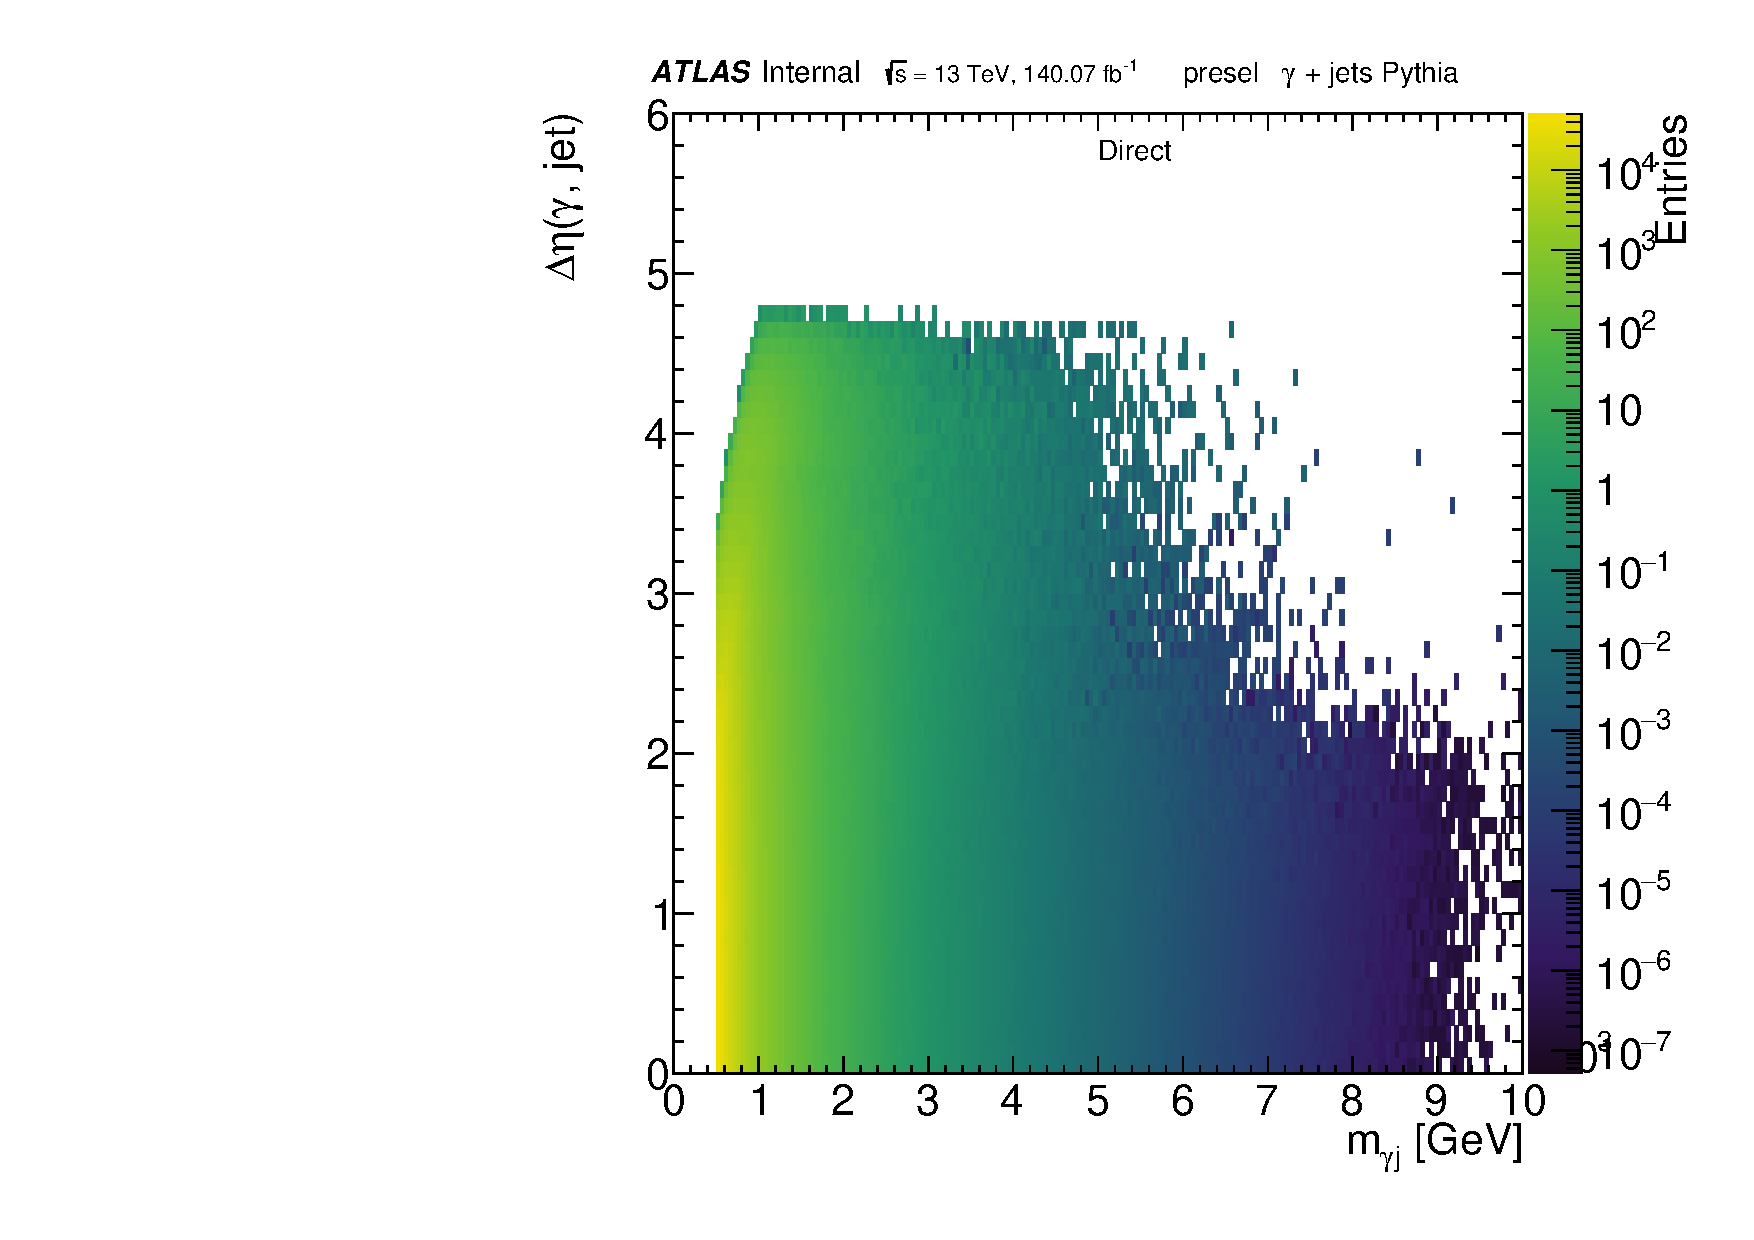
\includegraphics[width=\linewidth]{5_resonances/event_selection/deta/can2d__direct__presel__phjet_m_phjet_deta}
        \caption{\acf{DP}.}
        \label{fig:evt_selection:sr_opt:eta:deta:2d:direct}
    \end{subfigure}
    \hfill
    \begin{subfigure}[h]{0.49\linewidth}
        \centering
        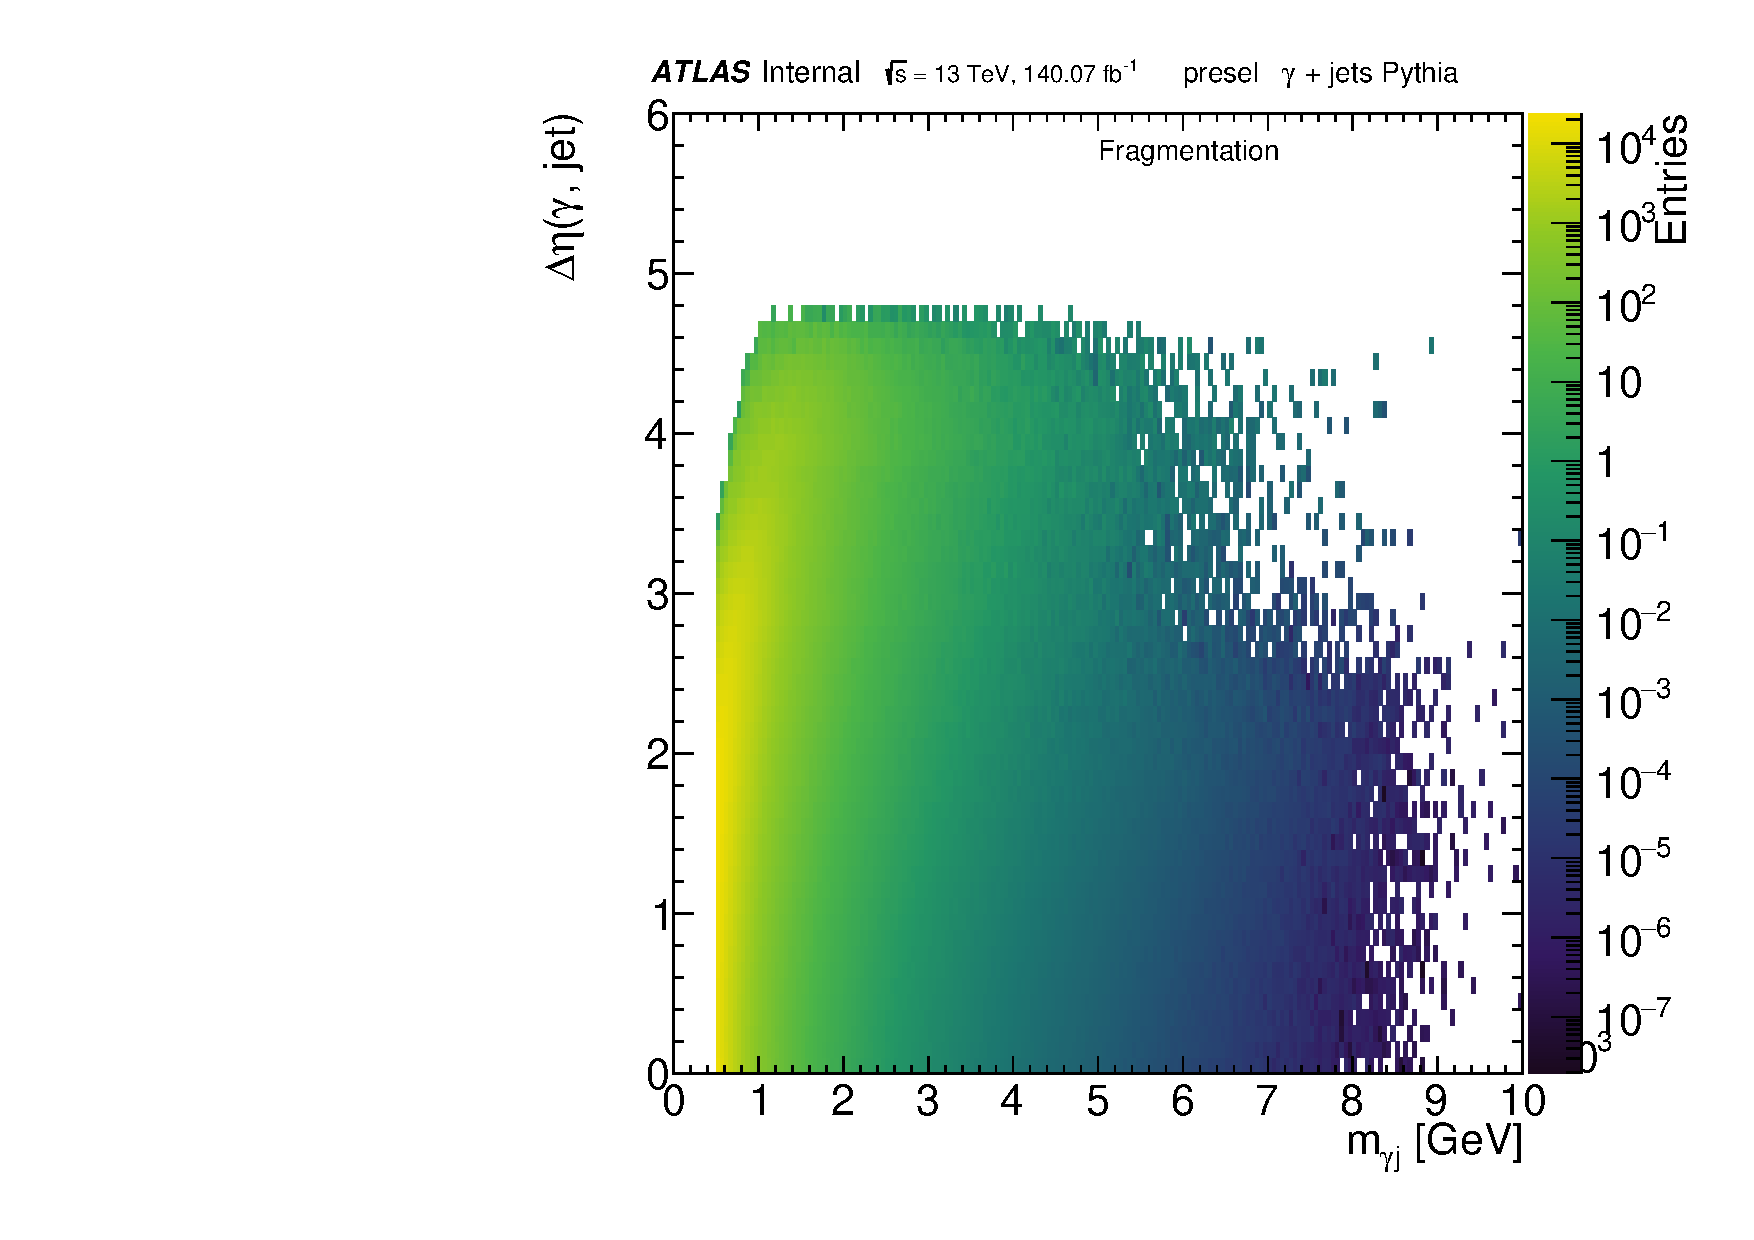
\includegraphics[width=\linewidth]{5_resonances/event_selection/deta/can2d__fragmentation__presel__phjet_m_phjet_deta}
        \caption{\acf{FP}.}
        \label{fig:evt_selection:sr_opt:eta:deta:2d:frag}
    \end{subfigure}
    \caption{Distribución bidimensional de \(\detayj-\myj\) para el fondo de \gammajet, separando entre \acp{DP} (izquierda) y \acp{FP} (derecha).}
    \label{fig:evt_selection:sr_opt:eta:deta:2d}
\end{figure}


La \Fig{\ref{fig:evt_selection:sr_opt:eta:deta:2d}} muestra la distribución bidimensional \Deta-\myj del fondo de \gammajet separando en eventos con \acp{DP} y \acp{FP}.
De estas distribuciones se desprende que hay una mayor concentración de eventos con valores más altos de \detayj para \acp{FP} que para \acp{DP}. Este escenario es cierto independientemente del valor de \myj pero es más prominente en la región de \(1 < \myj < 5~\tev\). Seleccionando eventos con \detayj bajo es posible rechazar una alta proporción de \acp{FP} y eventos del canal \(t\).

\begin{figure}[ht!]
    \centering
    \begin{subfigure}[h]{0.49\linewidth}
        \centering
        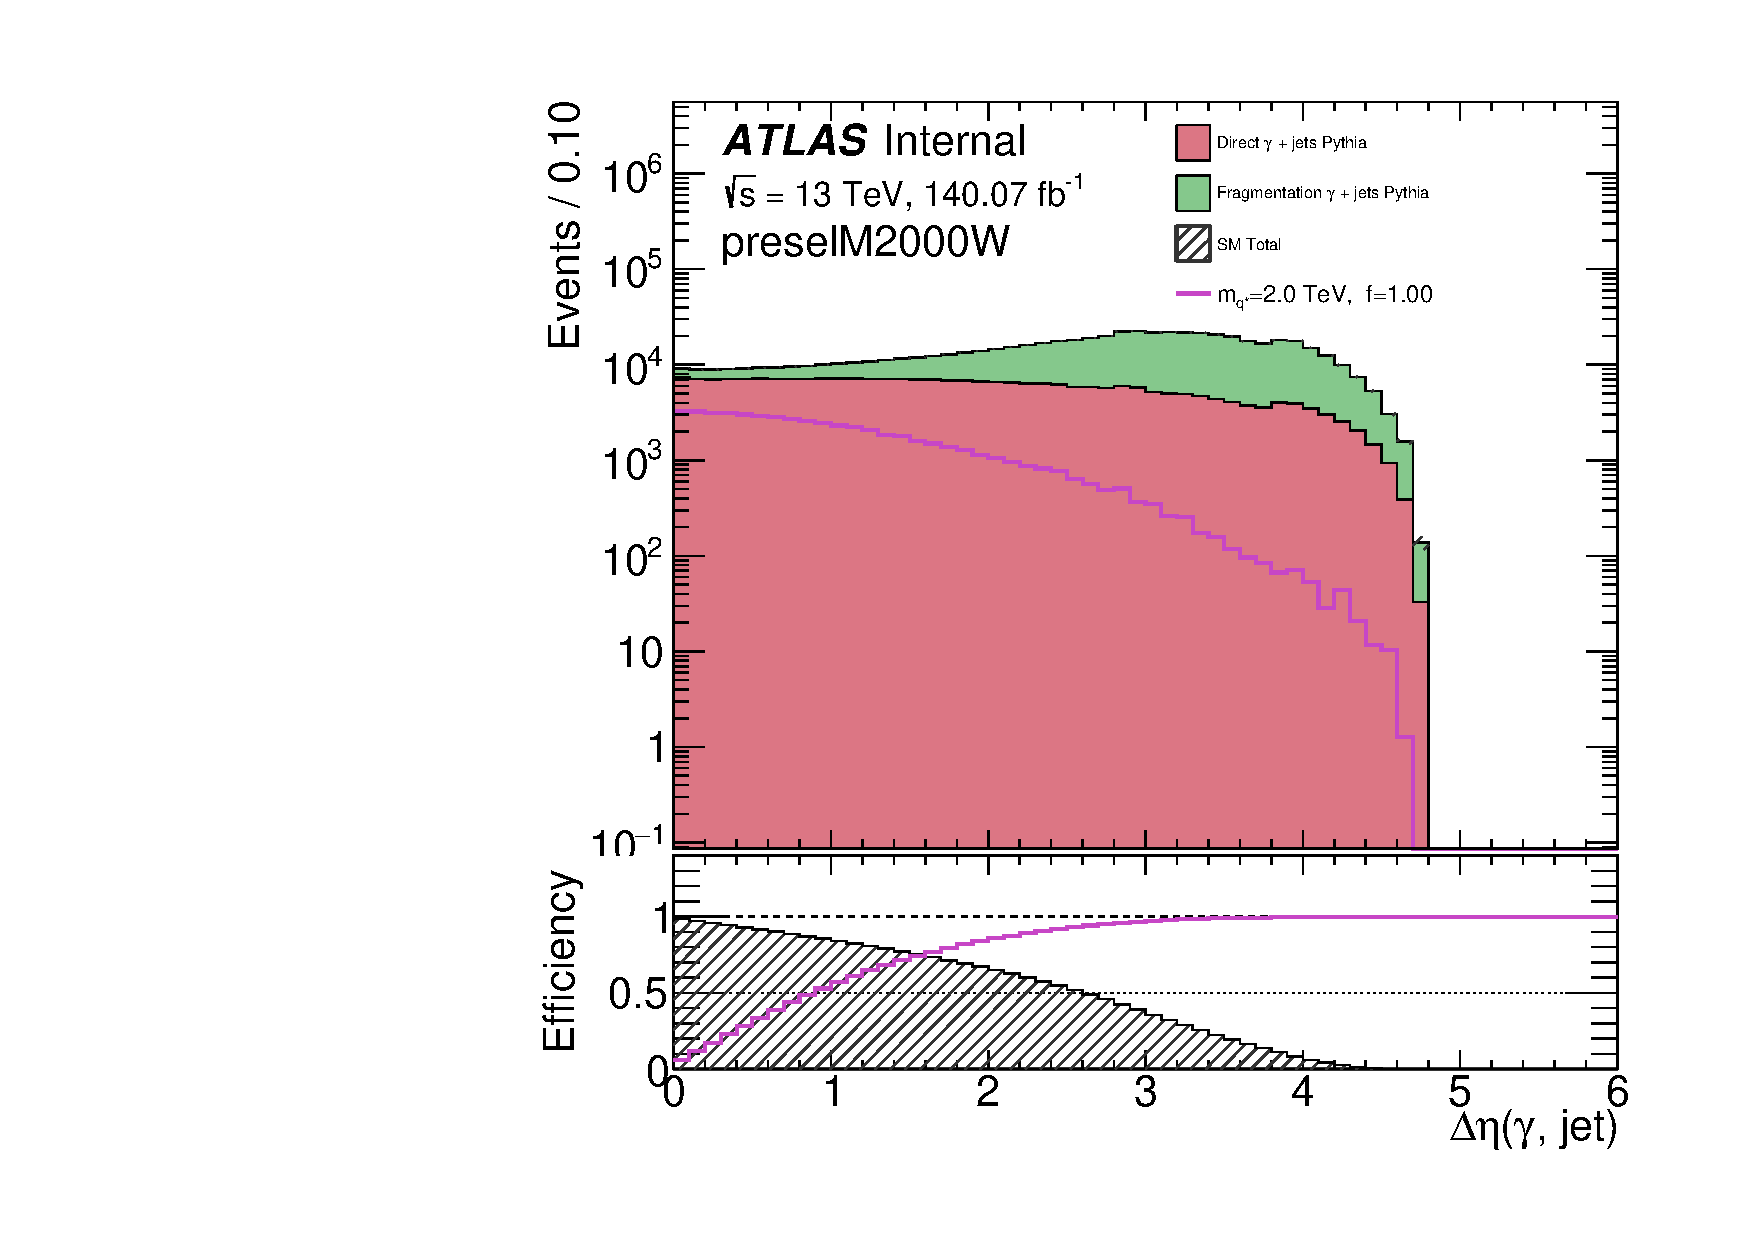
\includegraphics[width=\textwidth]{5_resonances/event_selection/deta/1d/preselM2000W/bkg_sig/1d/no_normalized/can__photonjet_Pythia_sig__preselM2000W__phjet_deta__wsignals_models__qStar_M2000__Run2__effrej}
        \caption{\(1000~\gev < \myj < 3000~\gev\)}
        \label{fig:evt_selection:sr_opt:eta:deta:1d:effrej_2000W}
    \end{subfigure}
    \hfill
    \begin{subfigure}[h]{0.49\linewidth}
        \centering
        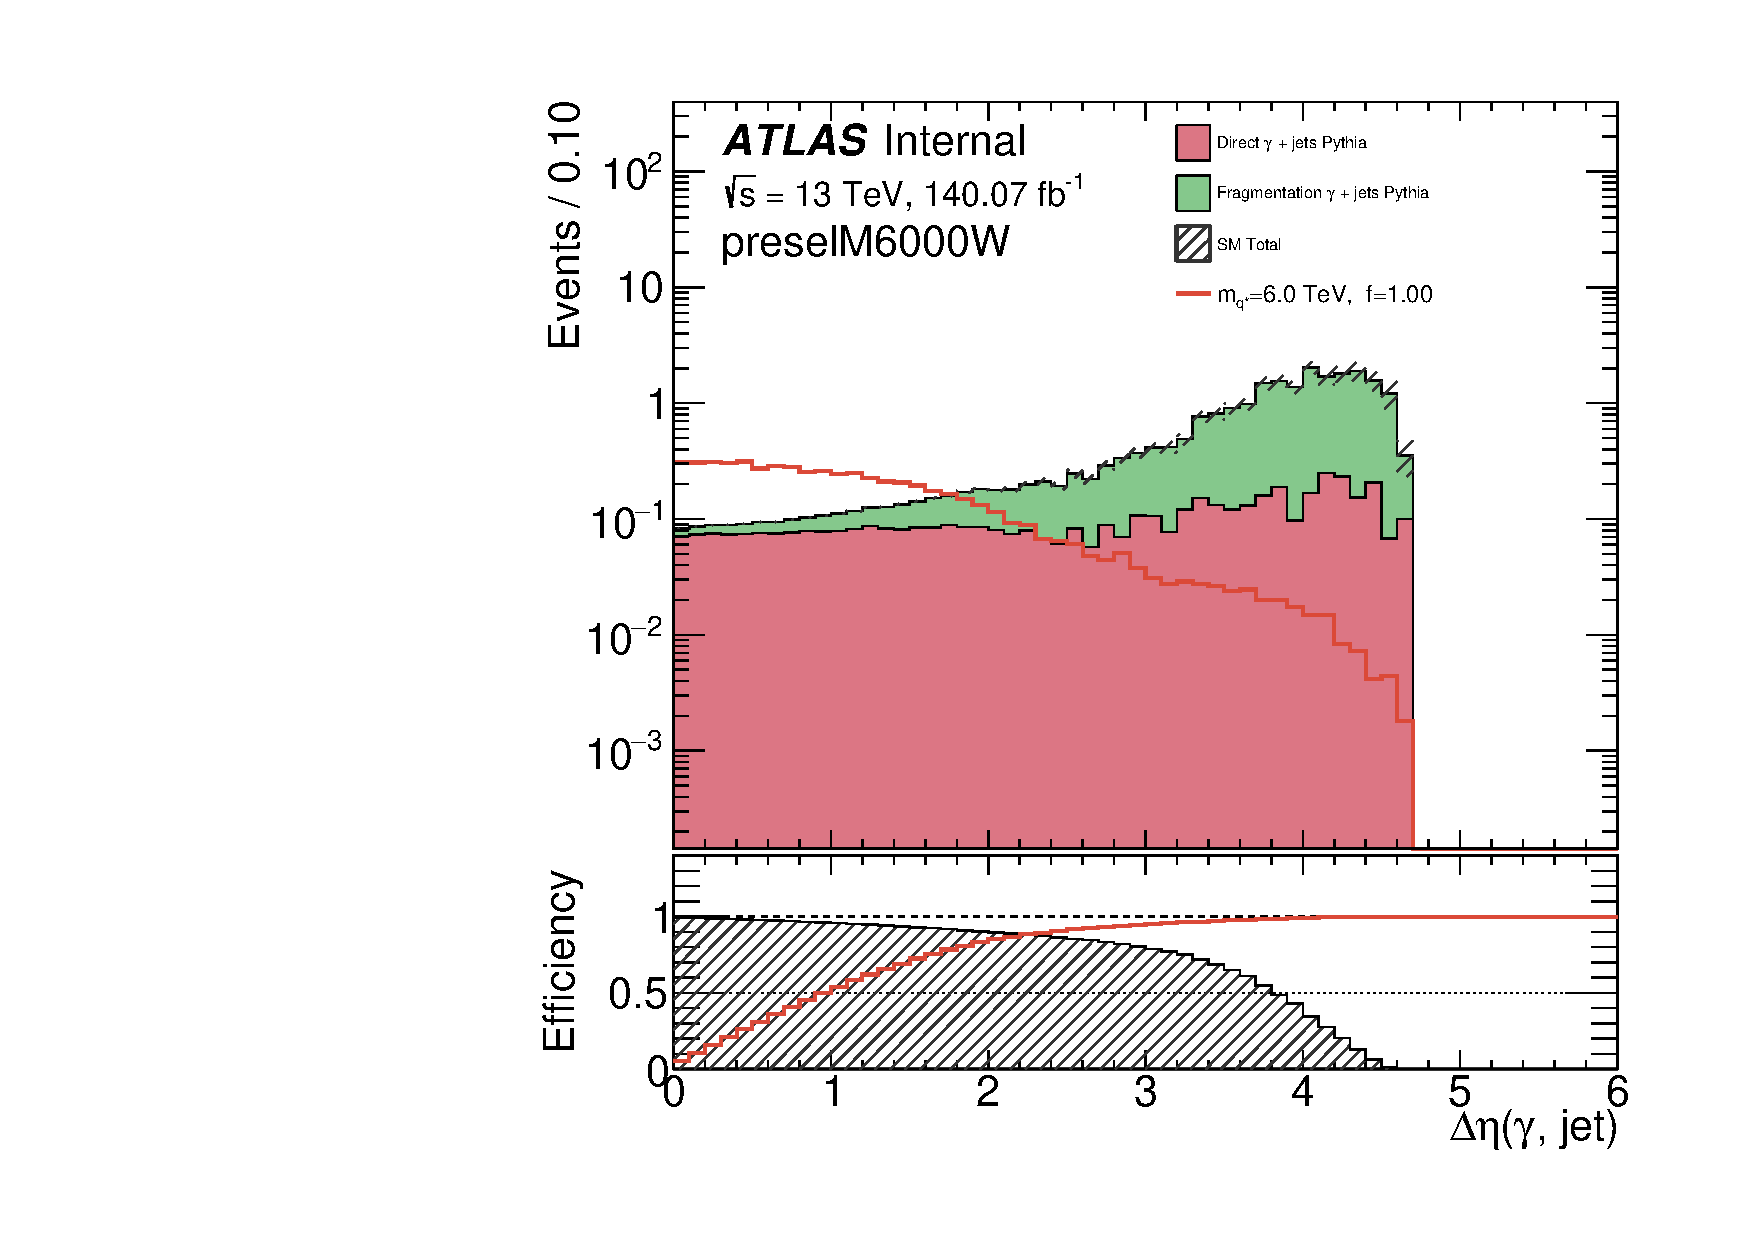
\includegraphics[width=\textwidth]{5_resonances/event_selection/deta/1d/preselM6000W/bkg_sig/1d/no_normalized/can__photonjet_Pythia_sig__preselM6000W__phjet_deta__wsignals_models__qStar_M6000__Run2__effrej}
        \caption{\(5000~\gev < \myj < 7000~\gev\)}
        \label{fig:evt_selection:sr_opt:eta:deta:1d:effrej_6000W}
    \end{subfigure}\\
    \begin{subfigure}[h]{0.49\linewidth}
        \centering
        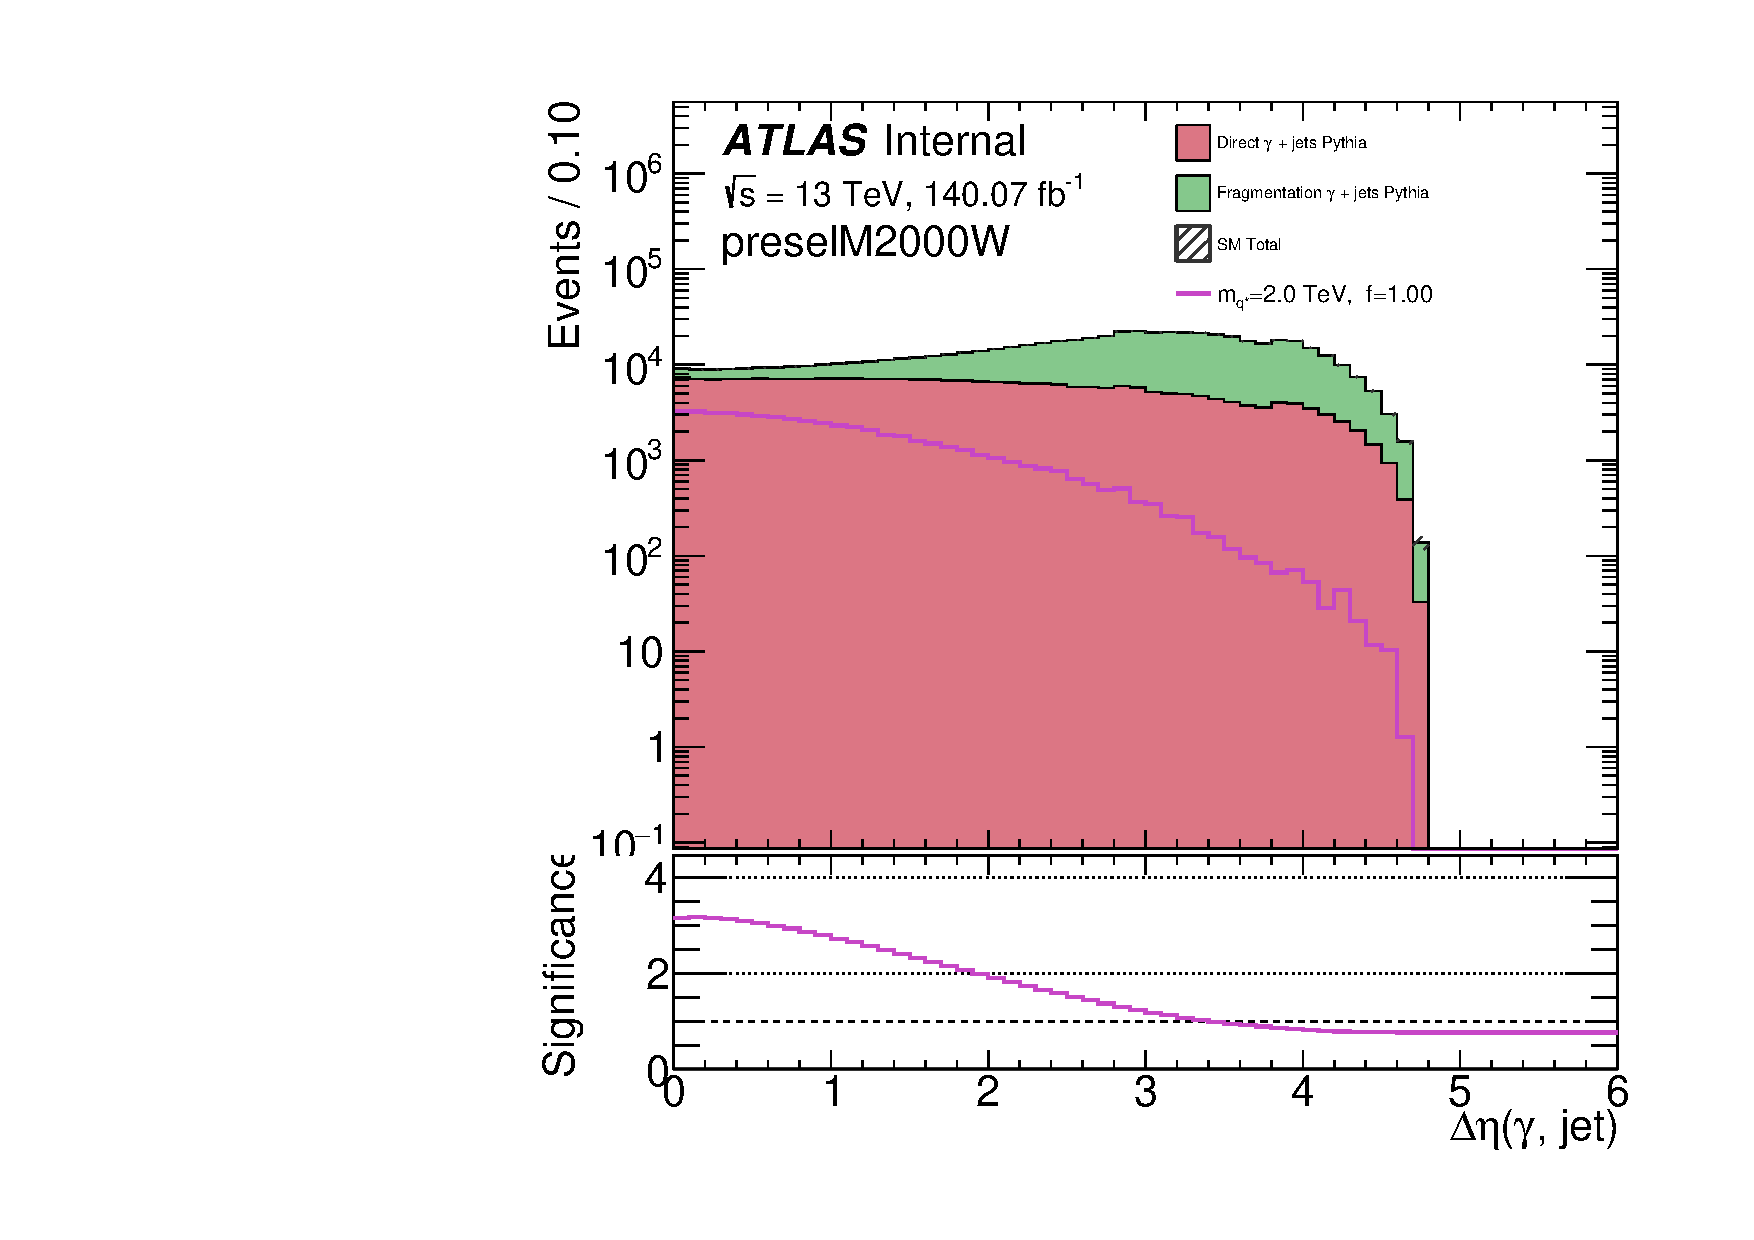
\includegraphics[width=\textwidth]{5_resonances/event_selection/deta/1d/preselM2000W/bkg_sig/1d/no_normalized/can__photonjet_Pythia_sig__preselM2000W__phjet_deta__wsignals_models__qStar_M2000__Run2__SB_significance}
        \caption{\(1000~\gev < \myj < 3000~\gev\)}
        \label{fig:evt_selection:sr_opt:eta:deta:1d:SB_2000W}
    \end{subfigure}
    \hfill
    \begin{subfigure}[h]{0.49\linewidth}
        \centering
        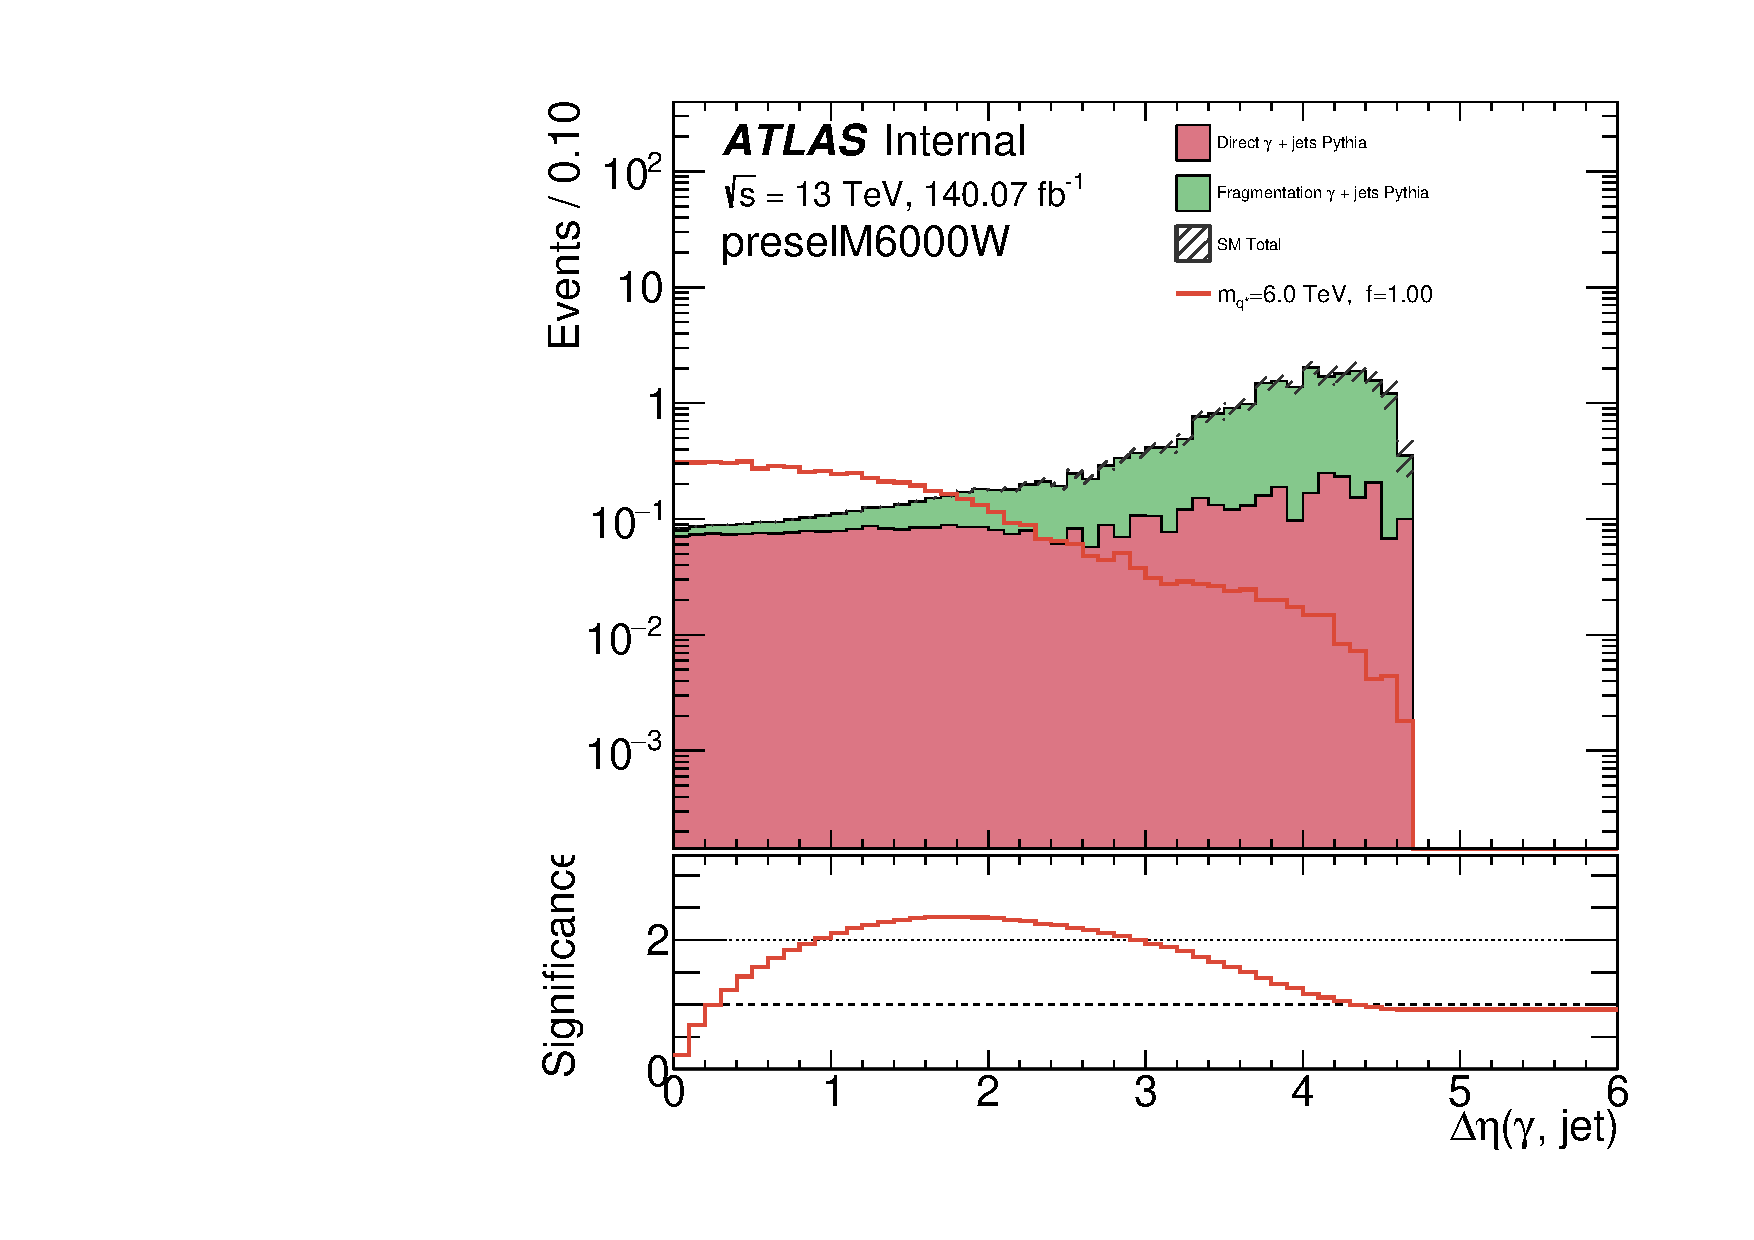
\includegraphics[width=\textwidth]{5_resonances/event_selection/deta/1d/preselM6000W/bkg_sig/1d/no_normalized/can__photonjet_Pythia_sig__preselM6000W__phjet_deta__wsignals_models__qStar_M6000__Run2__SB_significance}
        \caption{\(5000~\gev < \myj < 7000~\gev\)}
        \label{fig:evt_selection:sr_opt:eta:deta:1d:SB_6000W}
    \end{subfigure}
    \caption{Distribución de la variable \(\deta{\gamma}{j}\) en dos ventanas de \myj comparando le fondo con diferentes modelos de señal. El panel inferior de las \Figs{\ref{fig:evt_selection:sr_opt:eta:deta:1d:effrej_2000W}}{\ref{fig:evt_selection:sr_opt:eta:deta:1d:effrej_6000W}} muestran las eficiencias de las señales (líneas de colores), y el rechazo del fondo (histograma sombreado), si un corte del tipo \(\Deta < X\) es aplicado. Por otro lado, en las \Figs{\ref{fig:evt_selection:sr_opt:eta:deta:1d:SB_2000W}}{\ref{fig:evt_selection:sr_opt:eta:deta:1d:SB_6000W}}, los paneles inferiores muestran la significance de señal.}
    \label{fig:evt_selection:sr_opt:eta:deta:1d}
\end{figure}

Las comparaciones del fondo dominante obtenido con simulaciones con los modelos de señal utilizando esta variable se muestran en la \Fig{\ref{fig:evt_selection:sr_opt:eta:deta:1d}}. La selección en estas figuras corresponde a la selección de eventos con \(\mq - 1000 < \myj < \mq + 1000 ~\gev\), que consiste en una ventana de masa de \(2~\tev\) alrededor de la masa del modelo de señal.
El panel inferior en las \Figs{\ref{fig:evt_selection:sr_opt:eta:deta:1d:effrej_2000W}}{\ref{fig:evt_selection:sr_opt:eta:deta:1d:effrej_6000W}} muestra la eficiencia en las señales para las líneas coloreadas, mientras que el histograma sombreado muestra el rechazo de fondo si se aplica un corte del tipo \(\Deta < X\). De ellos se desprende que un corte de esta variable en \(\Deta \approx 1.6\) permitiría reducir considerablemente el fondo (\(\sim 80\%\)) manteniendo la mayoría de los eventos de señal (eficiencia \(60-80\%\)).
También se han llevado a cabo estudios que computan la significancia de este corte. Las \Figs{\ref{fig:evt_selection:sr_opt:eta:deta:1d:SB_2000W}}{\ref{fig:evt_selection:sr_opt:eta:deta:1d:SB_6000W}} muestran en los paneles inferiores la significancia de la señal para los mismos casos.
Exceptuando el corte trivial en \(\Deta = 0\), puede observarse que para valores altos de \myj puede alcanzarse la máxima significancia seleccionando eventos con \(\deta{\gamma}{j} \lesssim 1.6\), y por esta razón se ha optado por aplicar el corte \(\deta{\gamma}{j} < 1.6\) para el resto del análisis.
Otro aspecto importante que puede observarse en estas figuras es el hecho de que los eventos de fotones de fragmentación dominan en la región de alto \Deta, tal y como se preveía en la \Fig{\ref{fig:evt_selection:sr_opt:eta:deta:2d:frag}}. Aplicando este corte se logra entonces reducir en gran medida los eventos de \acp{FP}.


\subsubsection{Pseudorapidez del fotón y el jet}
\label{subsubsec:evt_selection:sr_opt:eta:etas}

En la región de baja masa \(\myj \lesssim 3~\tev\), se puede observar que hay una alta concentración de fondo con \(\etagam > 1.37\) y \(\etajet > 1.37\) en comparación con los modelos de señal, como se ve en la \Fig{\ref{fig:evt_selection:sr_opt:eta:etas:1d}}. Por este motivo, aplicando un corte en estas dos variables, la relación señal/fondo aumentaría sin afectar prácticamente la significancia de la señal ni en la eficiencia como se muestra en los paneles inferiores de las figuras. Por lo tanto, se decide eliminar los eventos con \(|\etagam| > 1.37\) y \(|\etajet| > 1.37\).

\begin{figure}[ht!]
    \centering
    \begin{subfigure}[h]{0.49\linewidth}
        \centering
        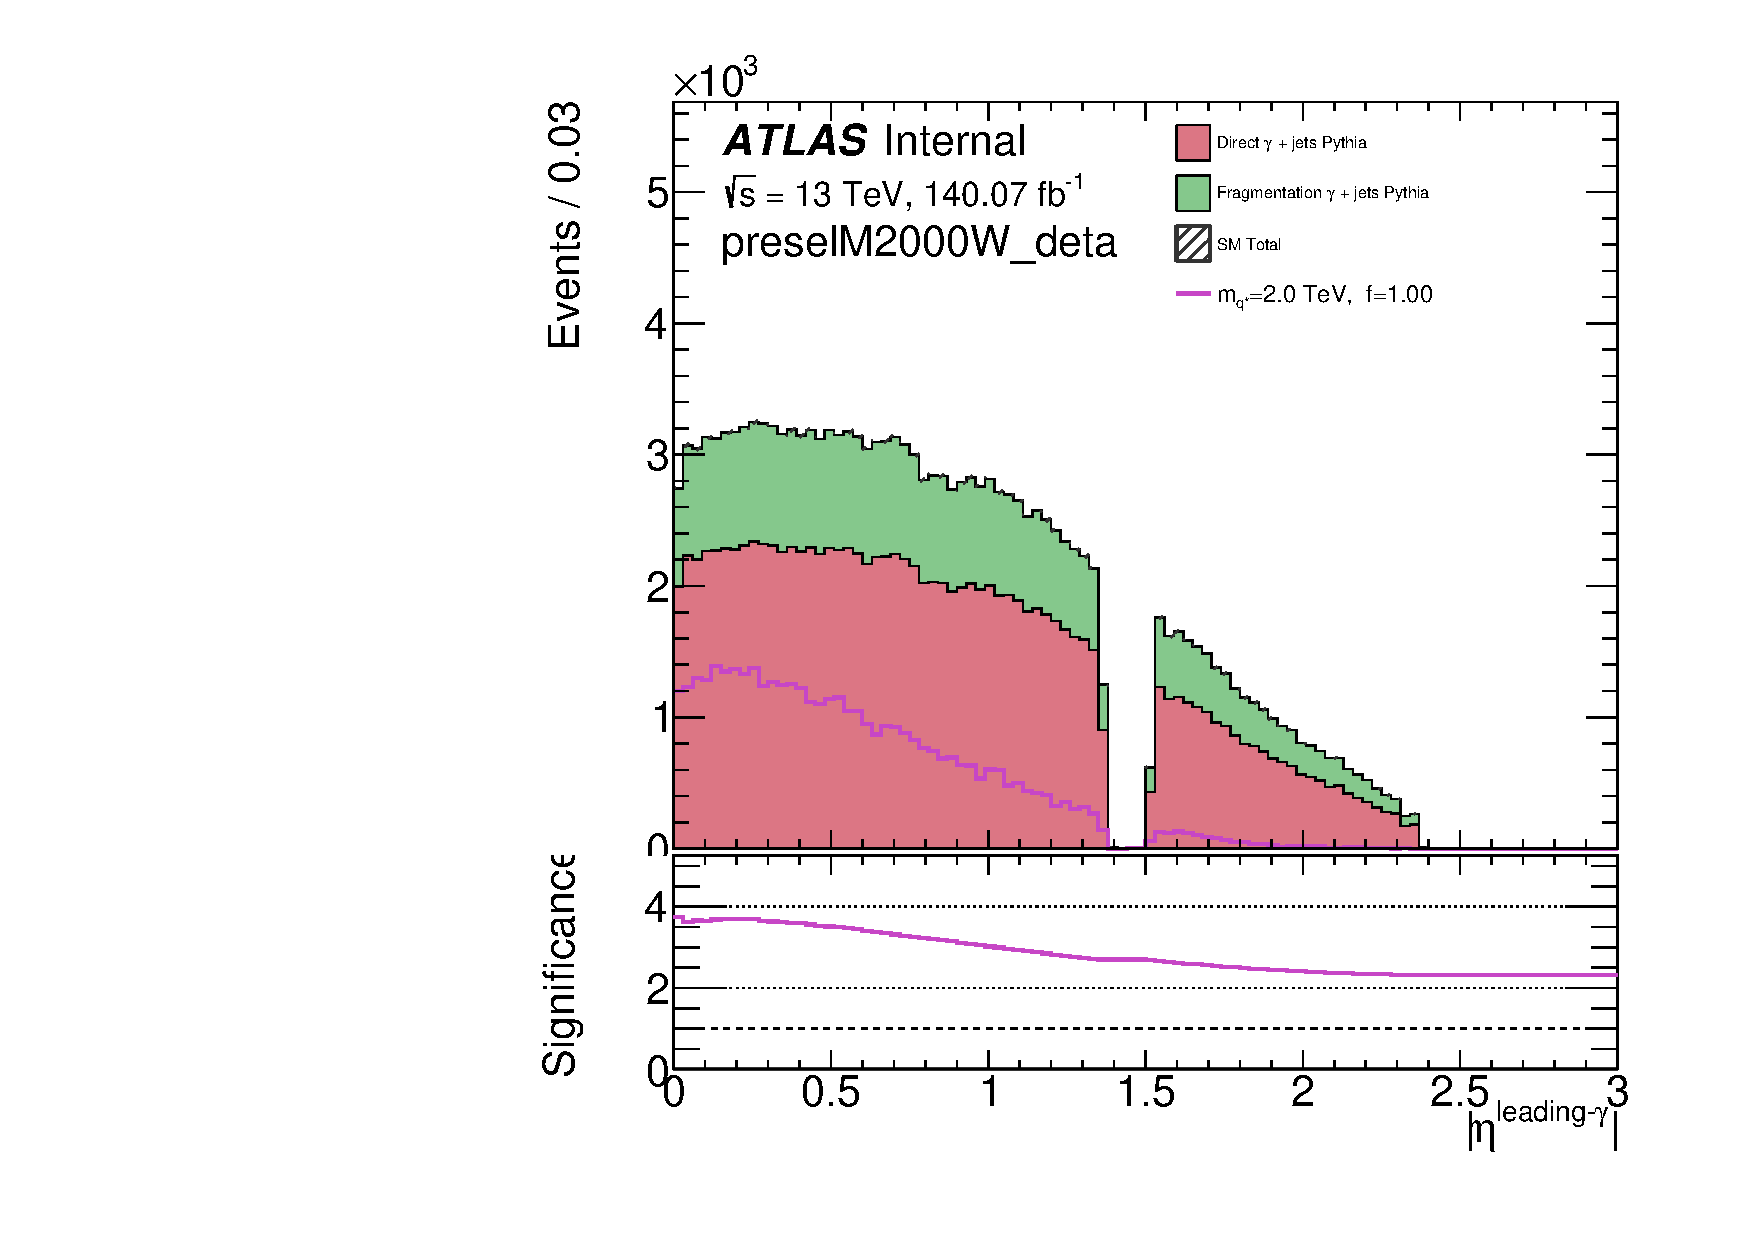
\includegraphics[width=\textwidth]{5_resonances/event_selection/eta/preselM2000W_deta/bkg_sig/1d/no_normalized/can__photonjet_Pythia_sig__preselM2000W_deta__absph_eta0__wsignals_models__qStar_M2000__Run2__SB_significance}
        \caption{\etagam}
        \label{fig:evt_selection:sr_opt:eta:etas:1d:ph}
    \end{subfigure}
    \hfill
    \begin{subfigure}[h]{0.49\linewidth}
        \centering
        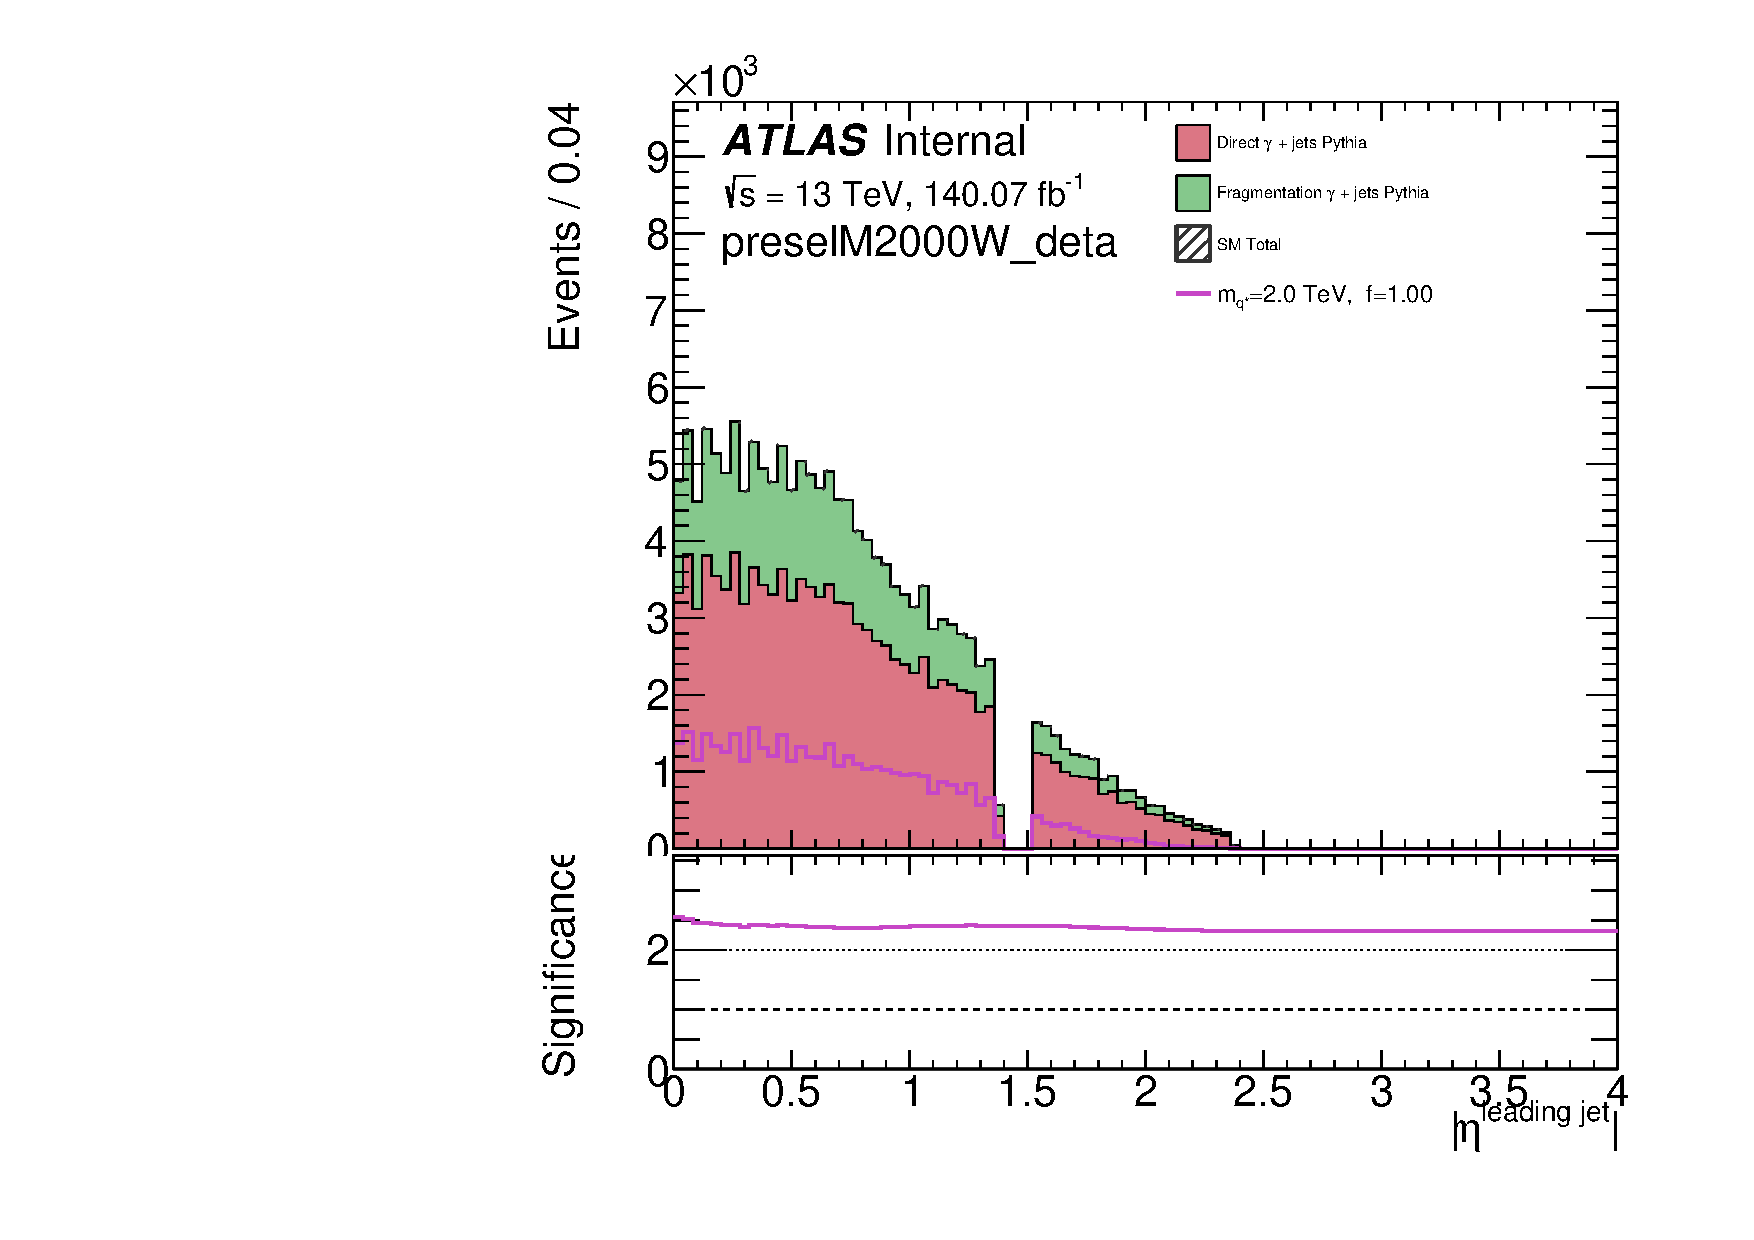
\includegraphics[width=\textwidth]{5_resonances/event_selection/eta/preselM2000W_deta/bkg_sig/1d/no_normalized/can__photonjet_Pythia_sig__preselM2000W_deta__absjet_eta0__wsignals_models__qStar_M2000__Run2__SB_significance}
        \caption{\etajet}
        \label{fig:evt_selection:sr_opt:eta:etas:1d:jet}
    \end{subfigure}
    \caption{Distribuciones de \etagam y \etajet en una ventana de masa \(1000~\gev < \myj < 3000~\gev\) comparando las señales con el fondo de \yj. Los paneles inferiores muestran la significancia de la señal sobre el fondo.}
    \label{fig:evt_selection:sr_opt:eta:etas:1d}
\end{figure}



\subsection{Aislamiento extendido}
\label{subsec:evt_selection:sr_opt:extended_iso}

Los algoritmos de reconstrucción, identificación y aislamiento de fotones actúan para reducir los fondos instrumentales (hadrones mal identificados) a un nivel insignificante, pero parte del fondo (\acp{FP} y jets falseando fotones) permanece.
Para reducir aún más estos fondos, se investiga la contribución a la energía de aislamiento del fotón leading de los jets cercanos a él después de aplicar todas las selecciones mostradas anteriormente.

\begin{figure}[ht!]
    \centering
    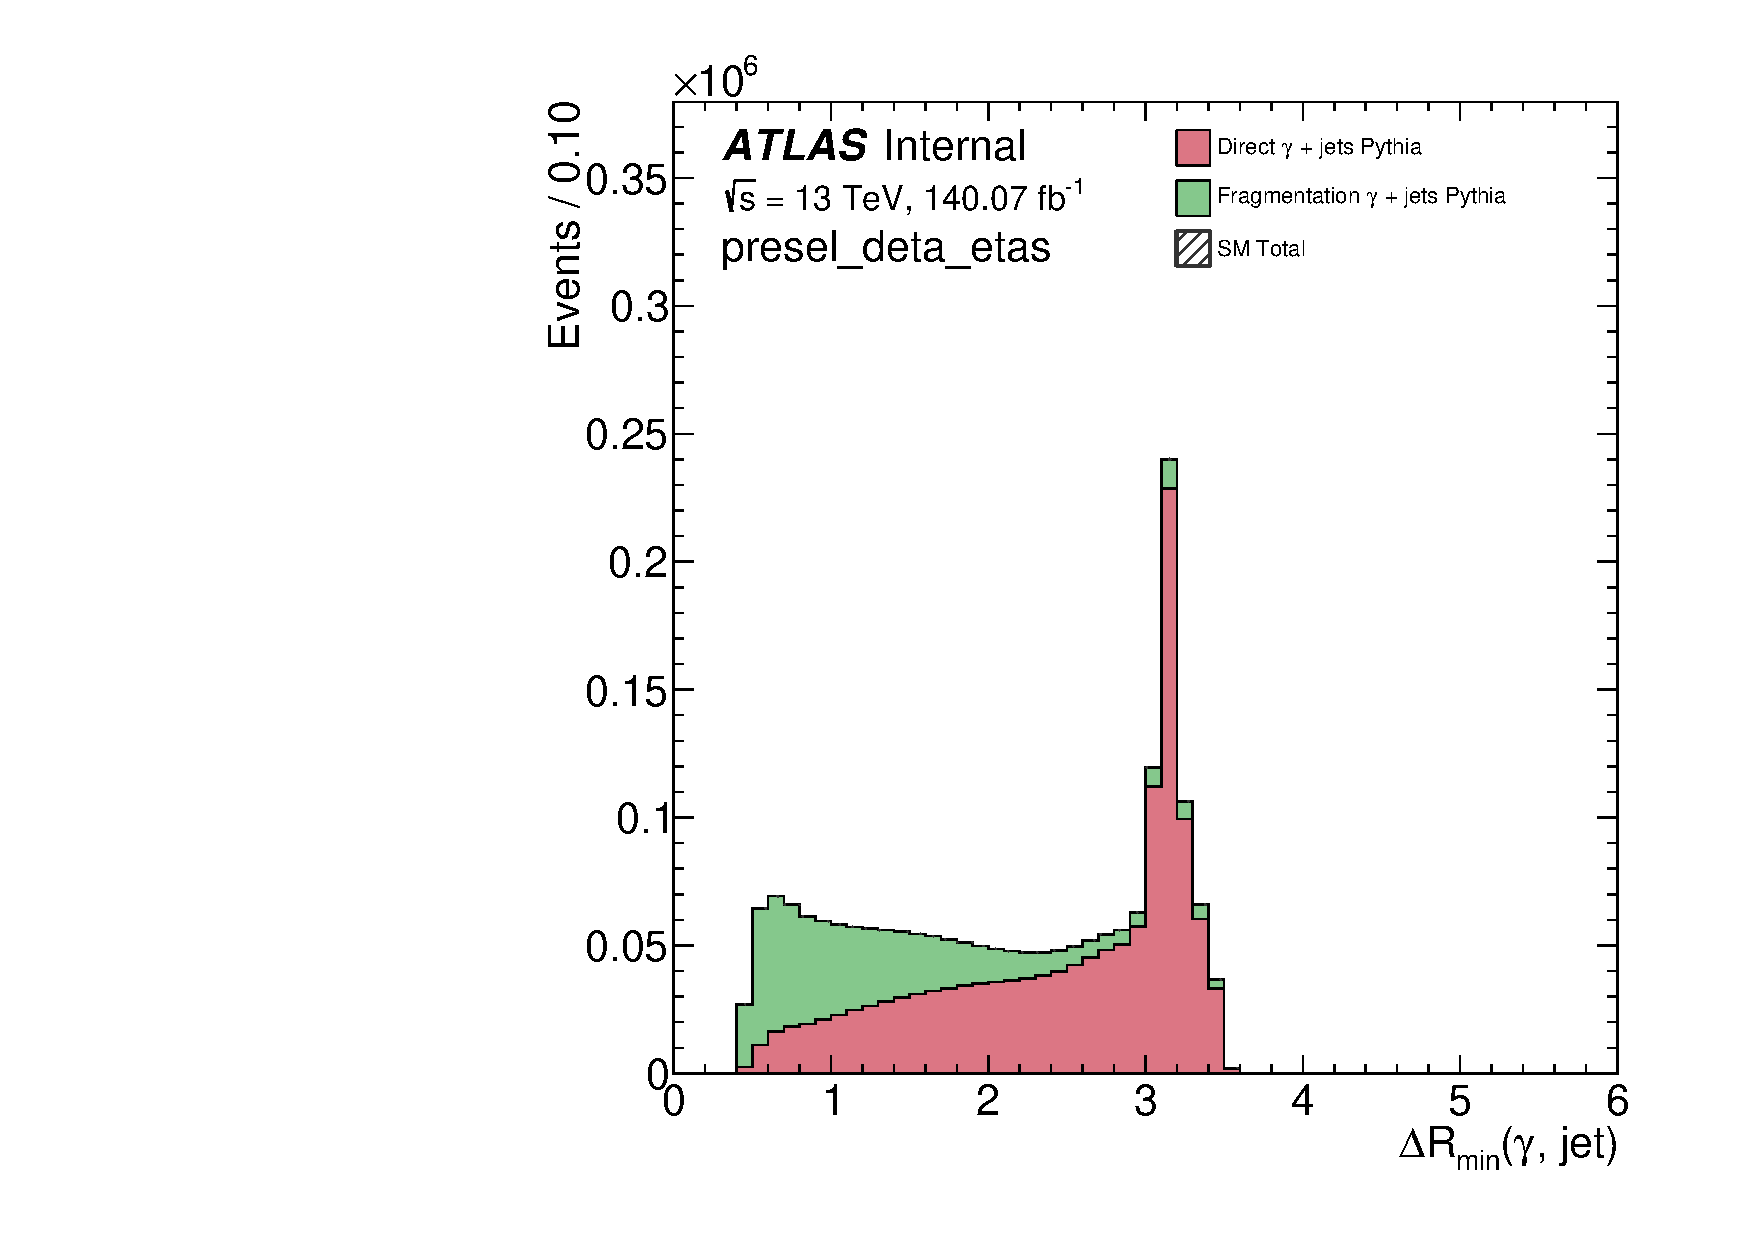
\includegraphics[width=0.49\linewidth]{5_resonances/event_selection/extended_iso/can__photonjet_Pythia__presel_deta_etas__phjet_drmin__Run2}
    \caption{Distribución de \(\DeltaR_{\text{min}}\) para el fondo de \gammajet. Esta variable muestra la distancia mínima entre el fotón leading con el jet más cercano a el. El histograma rojo muestra la contribución de los eventos de \acp{DP}, mientras que el verde muestra la contribución de \acp{FP}.}
    \label{fig:evt_selection:sr_opt:extended_iso:phjet_drmin}
\end{figure}
% \begin{figure}[ht!]
%     \centering
%     \begin{subfigure}[t]{0.49\linewidth}
%         \centering
%         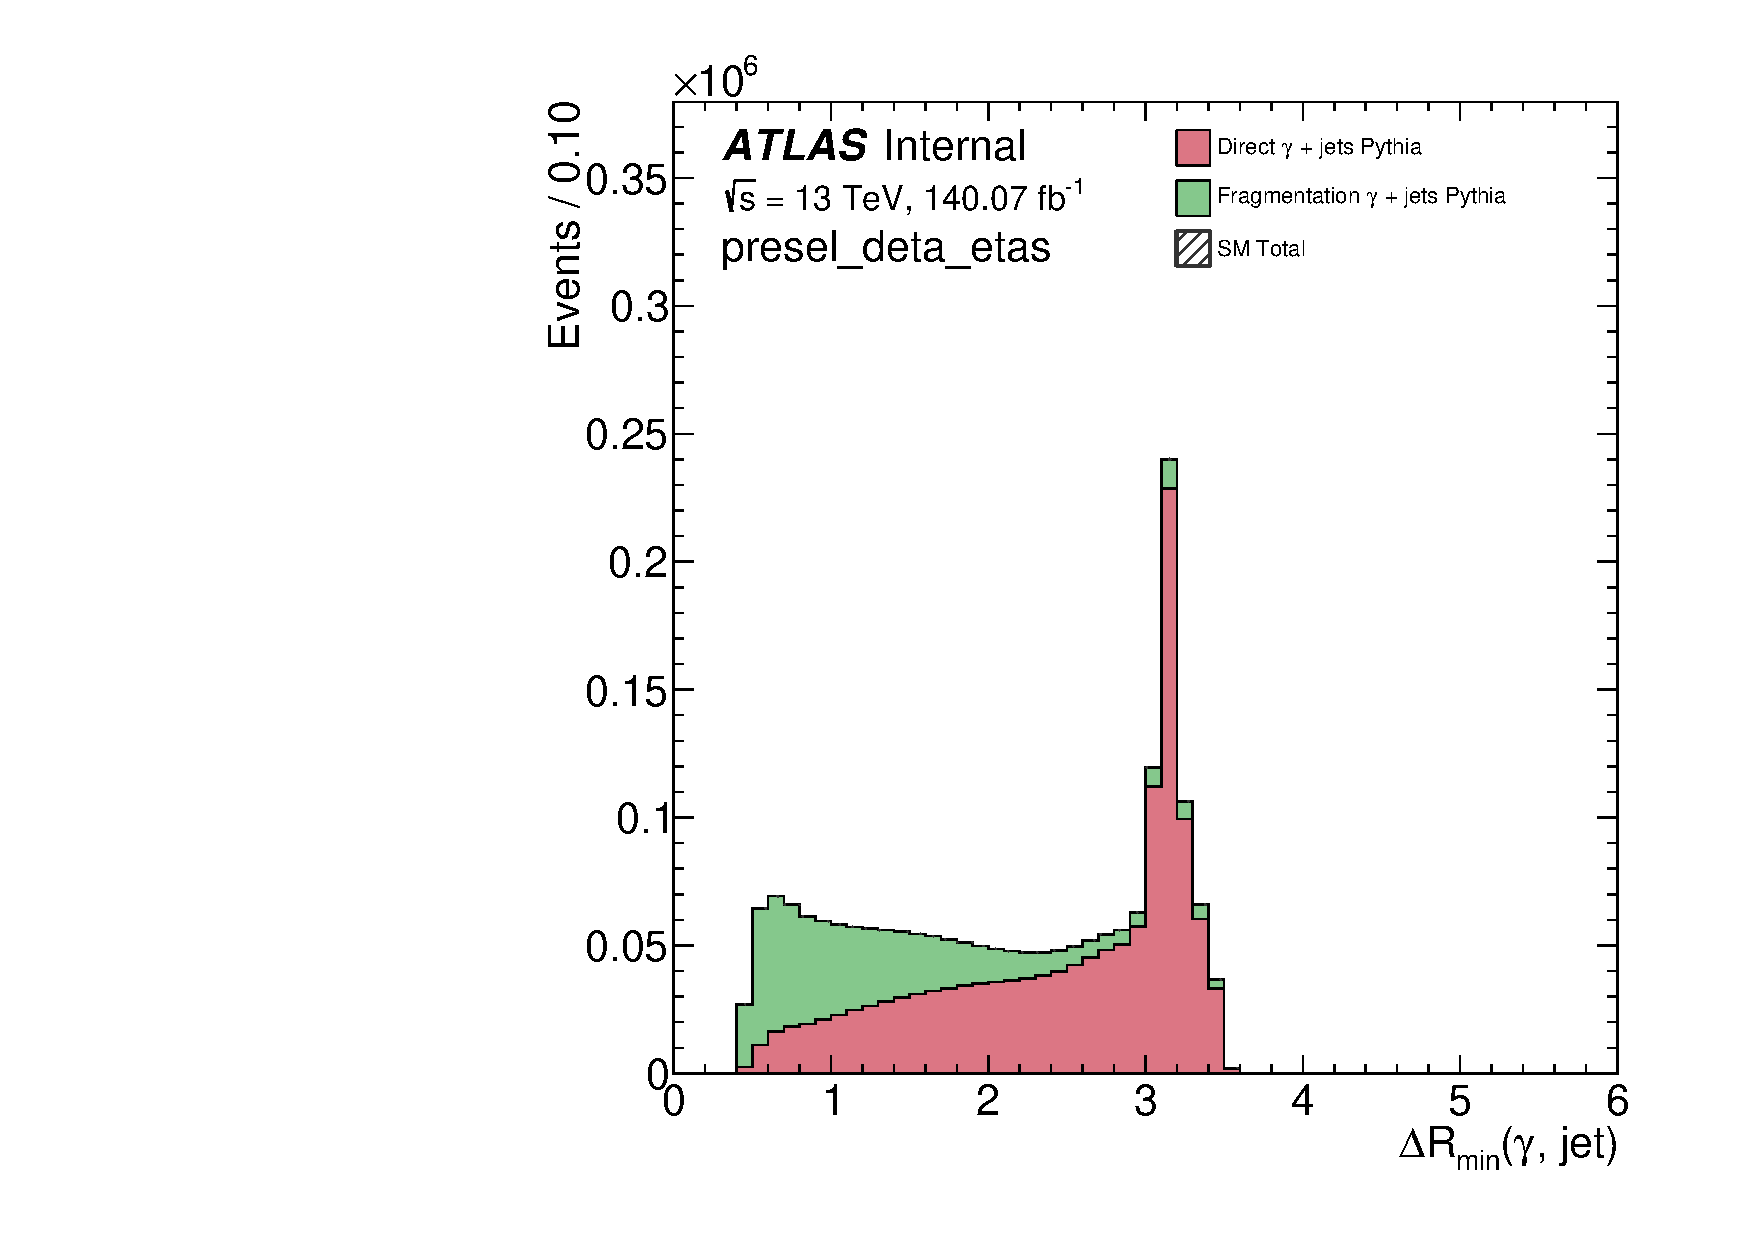
\includegraphics[width=\linewidth]{5_resonances/event_selection/extended_iso/can__photonjet_Pythia__presel_deta_etas__phjet_drmin__Run2}
%         \caption{Separación entre las contribuciones de fotones directos y de fragmentación.}
%         \label{fig:evt_selection:sr_opt:extended_iso:phjet_drmin:frag_direct}
%     \end{subfigure}
%     \hfill
%     \begin{subfigure}[t]{0.49\linewidth}
%         \centering
%         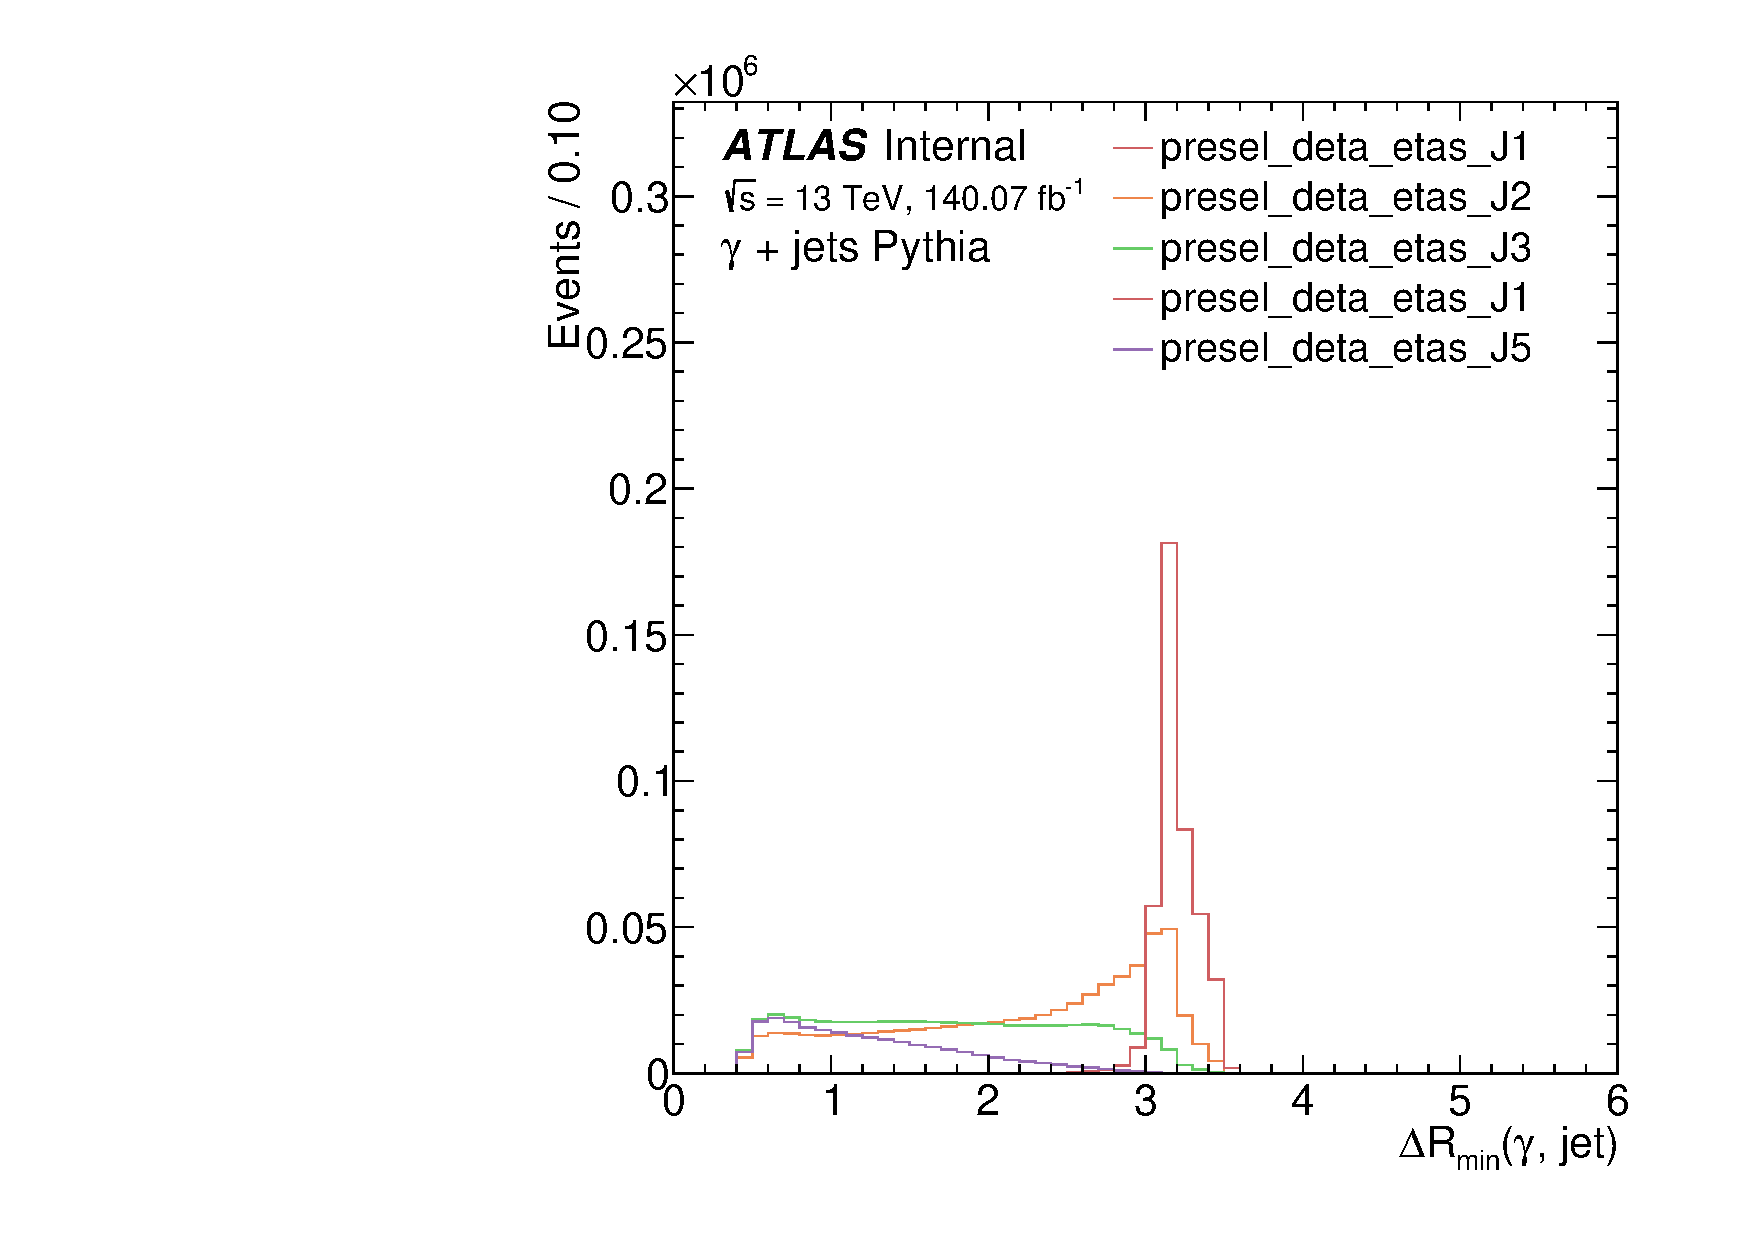
\includegraphics[width=\linewidth]{5_resonances/event_selection/extended_iso/can__photonjet_Pythia__phjet_drmin__regions_presel_deta_etas_J1_presel_deta_etas_J2_presel_deta_etas_J3_presel_deta_etas_J1_presel_deta_etas_J5__Run2}
%         \caption{Separación en la multiplicidad de los jets. El histograma con la línea roja muestra las contribuciones de los eventos en los que hay un sólo jet, la naranja donde hay dos, la verde donde hay 3 y la violeta donde hay más de 5.}
%         \label{fig:evt_selection:sr_opt:extended_iso:phjet_drmin:njets}
%     \end{subfigure}
%     \caption{Distribución de \(\DeltaR_{\text{min}}\) para el fondo de \gammajet. Esta variable muestra la distancia mínima entre el fotón leading con el jet más cercano a el.}
%     \label{fig:evt_selection:sr_opt:extended_iso:phjet_drmin}
% \end{figure}

En la \Fig{\ref{fig:evt_selection:sr_opt:extended_iso:phjet_drmin}} se muestra la distribución de \(\DeltaR_{\text{min}}\) separando entre eventos de \acp{DP} y \acp{FP}. Dicha variable mide la distancia angular entre el fotón leading y el jet más cercano. A partir de esta distribución es posible observar que la mayoría de los eventos muy cercanos al fotón (\(\DeltaR_{\text{min}}\) pequeño) son eventos de \acp{FP}.
% Además, se puede ver la contribución a dicha distribución separando los eventos con diferente multiplicidad de jets (\njet) mostrada en la \Fig{\ref{fig:evt_selection:sr_opt:extended_iso:phjet_drmin:njets}}. Se sabe que los eventos de fragmentación de fotones contienen más jets que los eventos procedentes de la producción directa de fotones, y a mayor multiplicidad de jets, mayores son las probabilidades de que un jet esté muy cerca del fotón, contribuyendo a la energía de aislamiento del mismo.


\begin{figure}[ht!]
    \centering
    \begin{subfigure}[t]{0.49\linewidth}
        \centering
        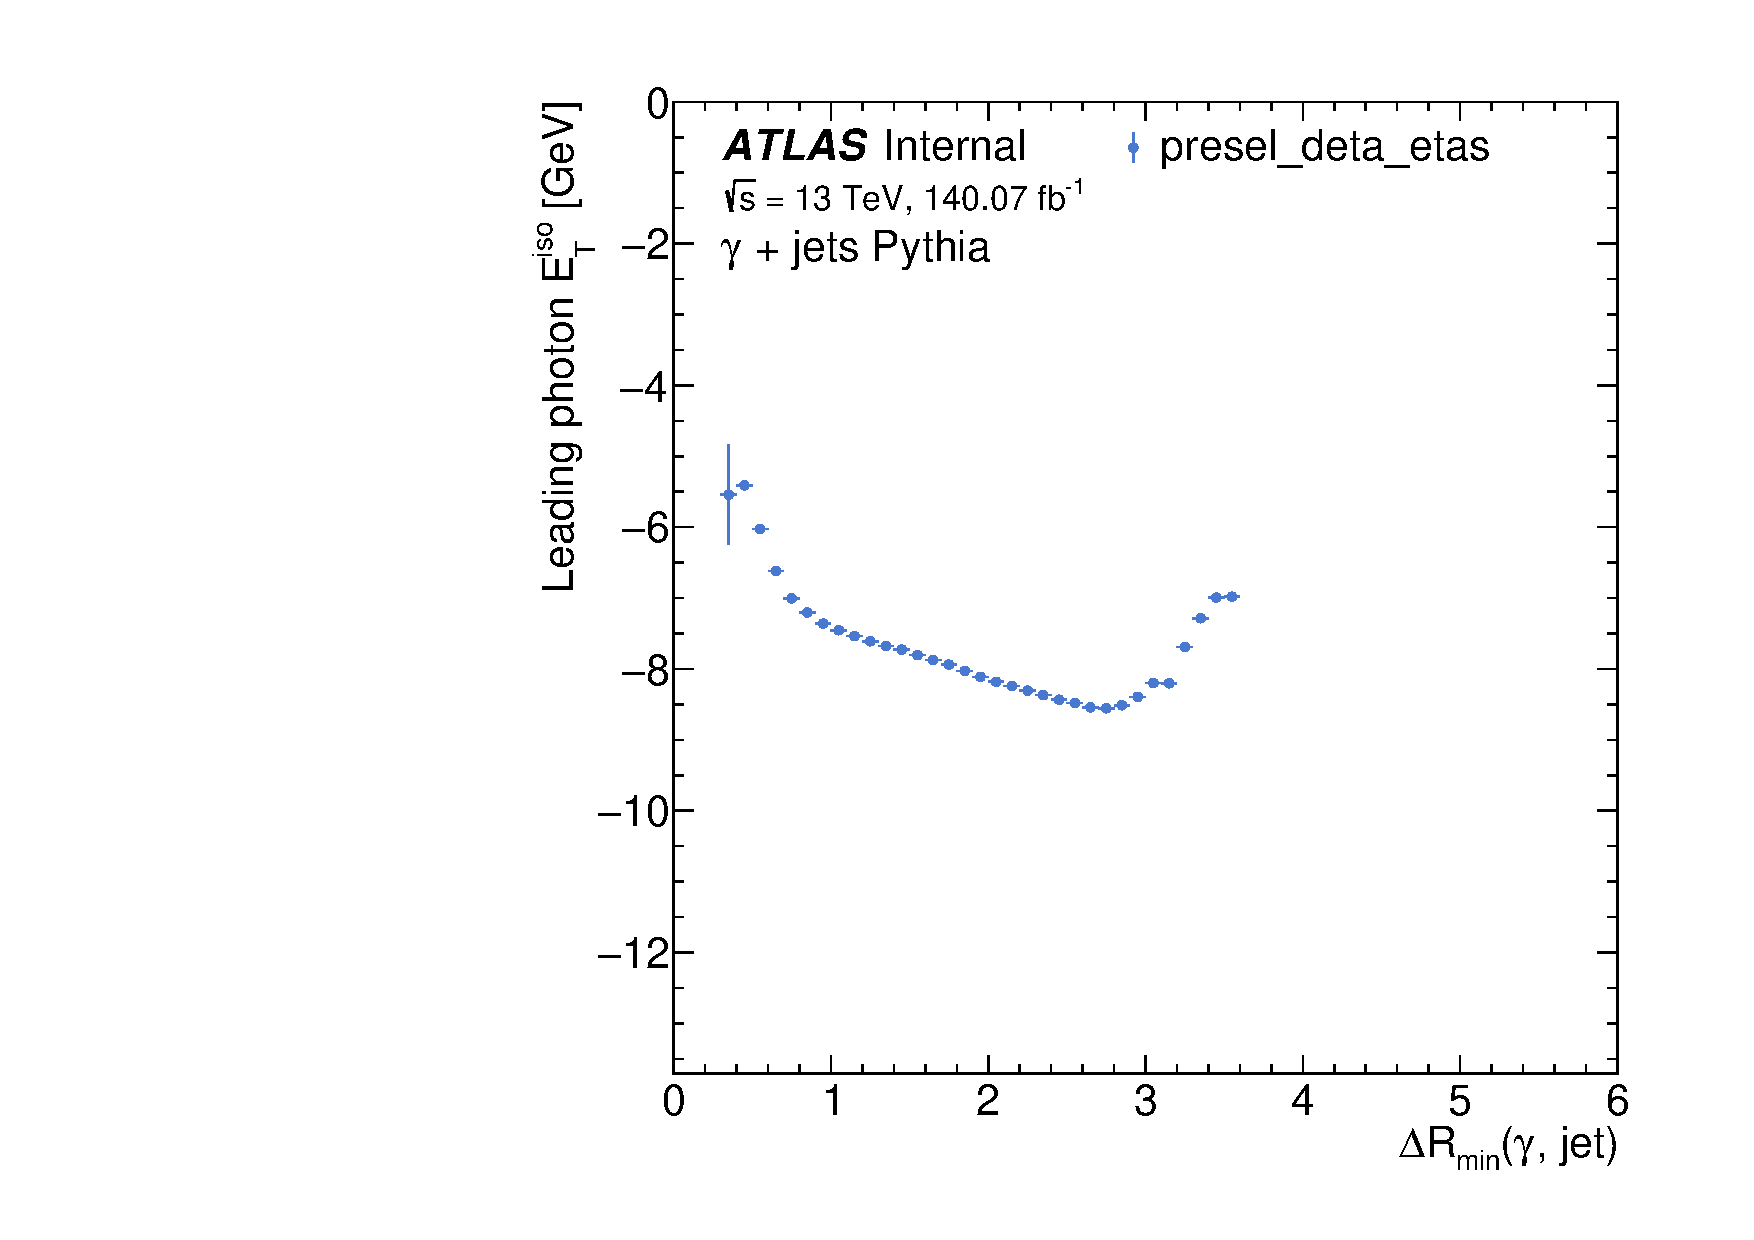
\includegraphics[width=\linewidth]{5_resonances/event_selection/extended_iso/can__photonjet_Pythia__phjet_drmin_ph_caloiso0__regions_presel_deta_etas__Run2}
        \caption{Contribución total de eventos de \acp{DP}+\acp{FP}.}
        \label{fig:evt_selection:sr_opt:extended_iso:phjet_drmin:etiso:full}
    \end{subfigure}
    \hfill
    \begin{subfigure}[t]{0.49\linewidth}
        \centering
        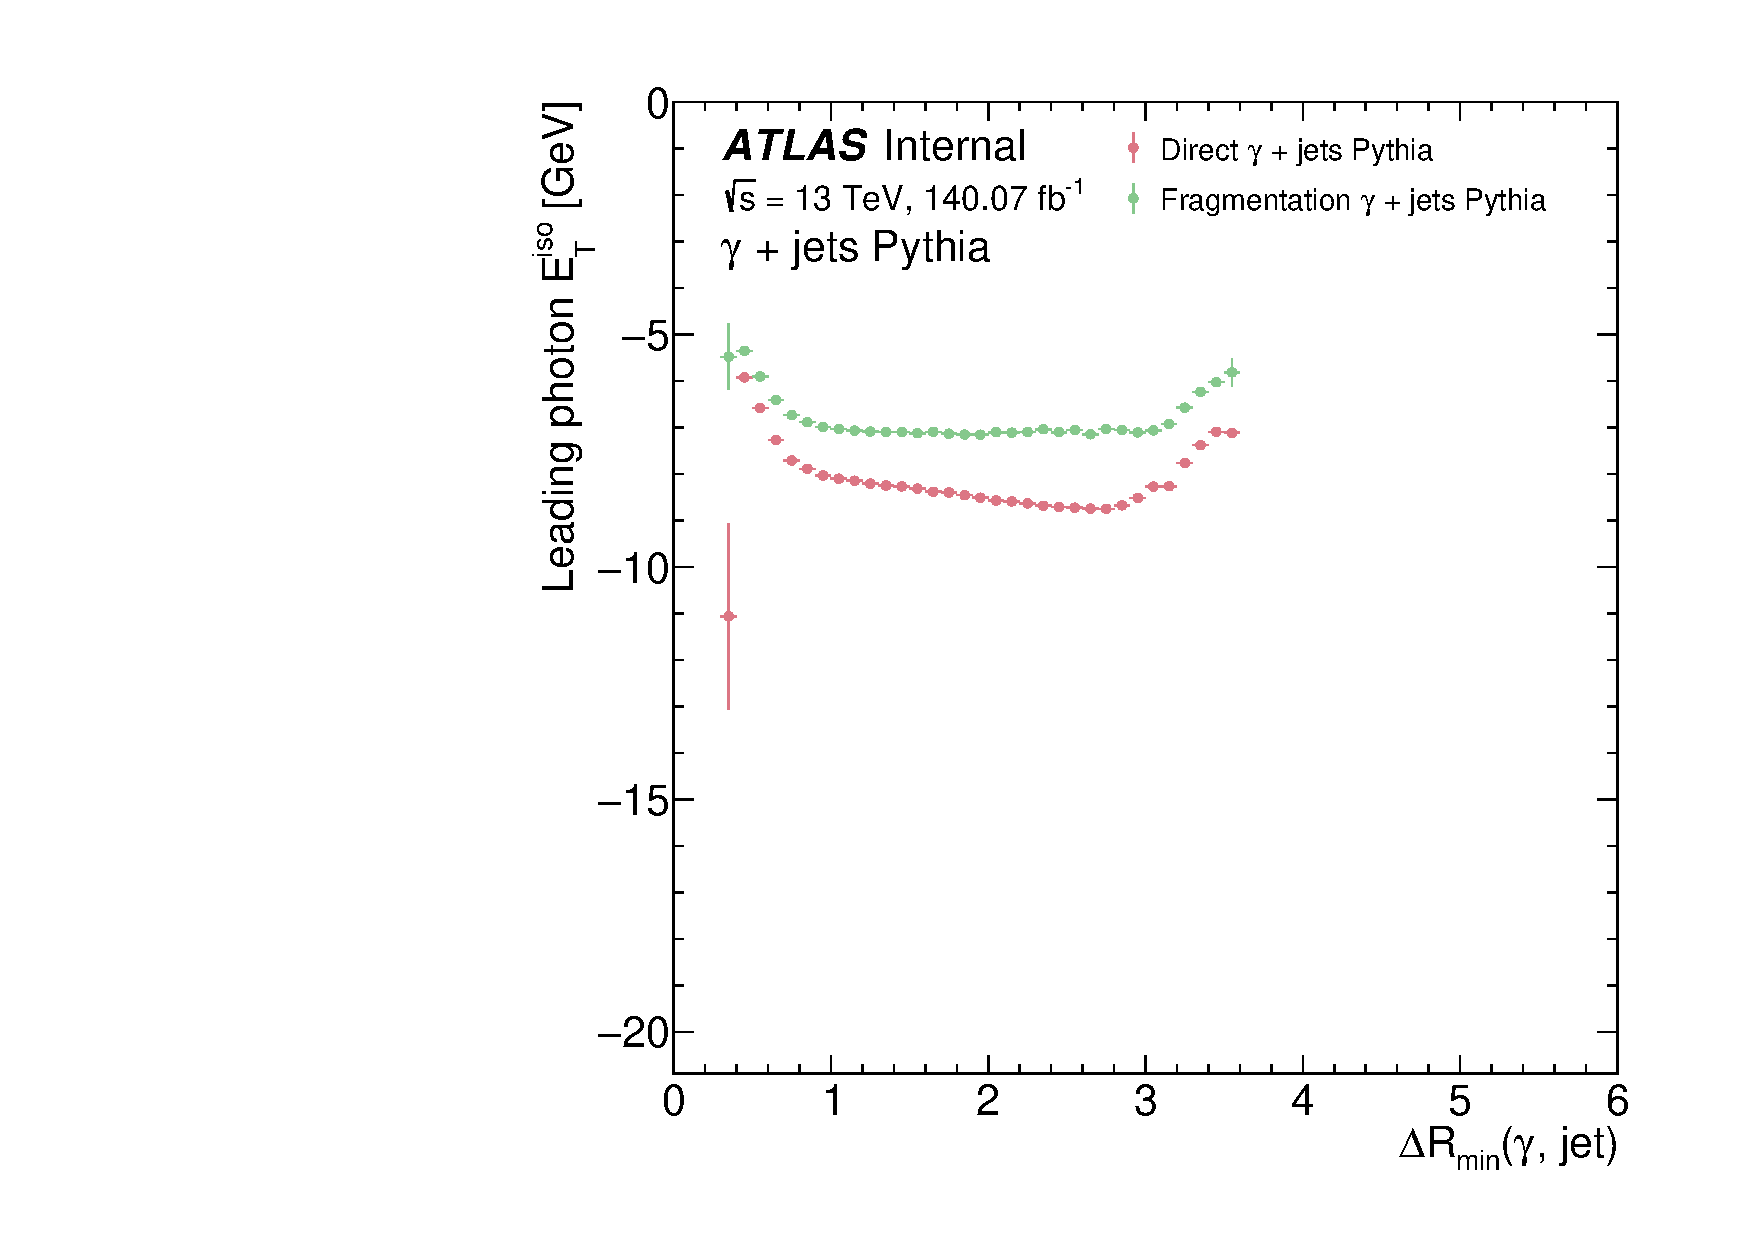
\includegraphics[width=\linewidth]{5_resonances/event_selection/extended_iso/can__photonjet_Pythia__phjet_drmin_ph_caloiso0__presel_deta_etas__Run2}
        \caption{Contribuciones de \acp{DP} y de \acp{FP} por separado.}
        \label{fig:evt_selection:sr_opt:extended_iso:phjet_drmin:etiso:separated}
    \end{subfigure}
    \caption{Distribución de la energía de aislamiento \(\etiso\) como función de \(\DeltaR_{\text{min}}\).}
    \label{fig:evt_selection:sr_opt:extended_iso:phjet_drmin:etiso}
\end{figure}

Para estudiar la contribución a la energía de aislamiento del fotón de estos jets se presenta la \Fig{\ref{fig:evt_selection:sr_opt:extended_iso:phjet_drmin:etiso:full}} con el valor medio de la energía de aislamiento del fotón en función de \(\DeltaR_{\text{min}}\). Los jets que se encuentran muy cerca del fotón contribuyen en gran medida a esta energía, especialmente los jets con \(\DeltaR (\gamma, j) < 1.0\), valor al que la energía comienza a aumentar drásticamente. Este comportamiento también se presenta por separado para la producción de \acp{DP} y de \acp{FP} en la \Fig{\ref{fig:evt_selection:sr_opt:extended_iso:phjet_drmin:etiso:separated}}, de los cuales la mayor contribución a la energía viene dada por los eventos de \acp{FP}.
En consecuencia, se considera un corte de esta variable en \(\DeltaR (\gamma, j) \geq 1.0\) para reducir los eventos de \acp{FP} y obtener una muestra de fotones más limpia.






\subsection{Momento transverso del jet}
\label{subsec:evt_selection:sr_opt:jet_pt}


Después de aplicar todos los cortes mencionados, una característica clave observada en los eventos de \acp{FP} es que hay una gran proporción de eventos en los que el jet leading lleva mucho más momento que el fotón leading. En una producción directa ideal de fotones, que es lo que se pretende con esta selección de eventos, tanto el fotón como el jet llevan aproximadamente el mismo \pt. Para estudiar si una selección basada en el jet y el fotón \pt es factible, se muestran las distribuciones \ptgam vs \ptjet en la \Fig{\ref{fig:evt_selection:sr_opt:jet_pt:ptgam_ptjet}} tanto para \acp{DP} como de \acp{FP}. De estas figuras se observa claramente que la producción de \acp{FP} es la que contribuye a tener eventos con \(\ptjet \gg \ptgam\).


\begin{figure}[ht!]
    \centering
    \begin{subfigure}[h]{0.49\linewidth}
        \centering
        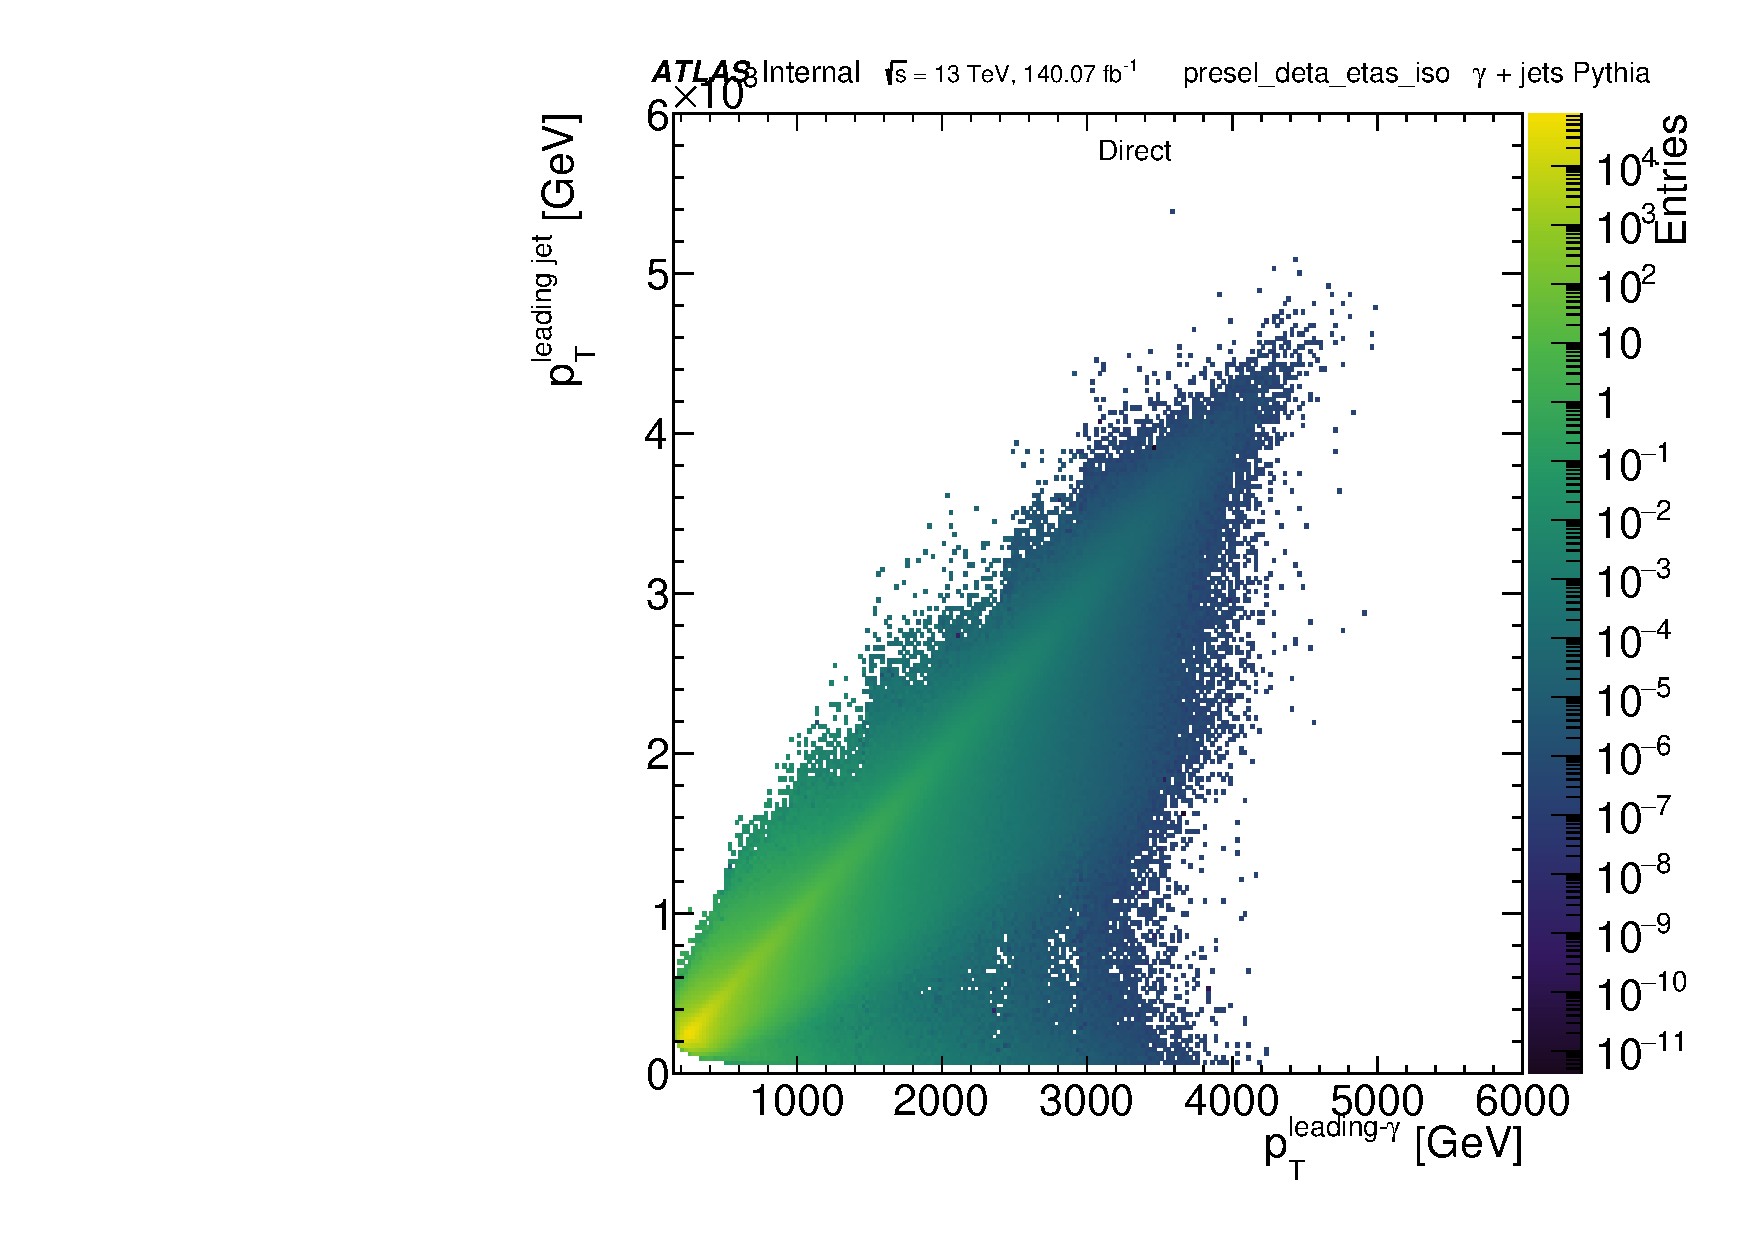
\includegraphics[width=\linewidth]{5_resonances/event_selection/jet_pt/presel_deta_etas_iso/bkg/2d/can2d__direct__presel_deta_etas_iso__ph_pt0_jet_pt0}
        \caption{\acp{DP}.}
    \end{subfigure}
    \hfill
    \begin{subfigure}[h]{0.49\linewidth}
        \centering
        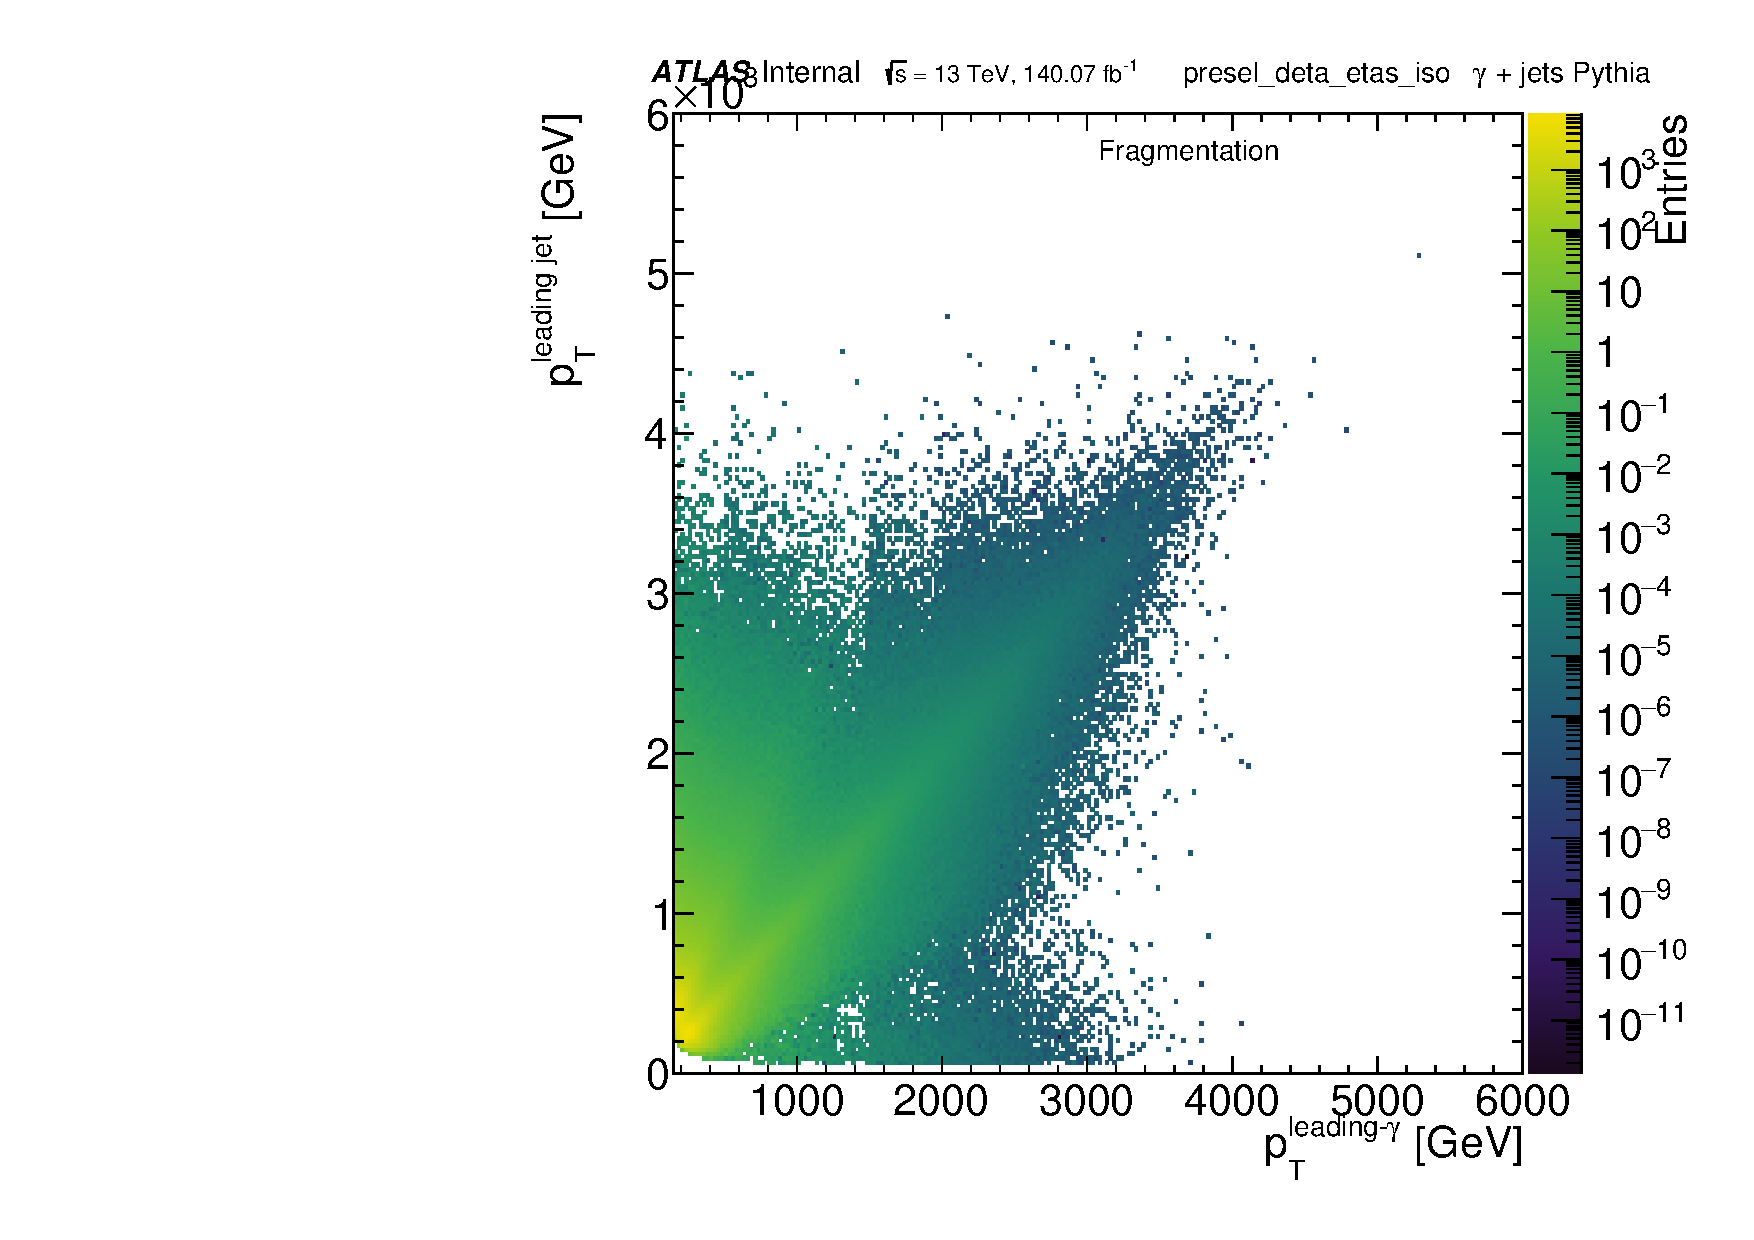
\includegraphics[width=\linewidth]{5_resonances/event_selection/jet_pt/presel_deta_etas_iso/bkg/2d/can2d__fragmentation__presel_deta_etas_iso__ph_pt0_jet_pt0}
        \caption{\acp{FP}.}
    \end{subfigure}
    \caption{Distribución bidimensional \ptgam-\ptjet para \acp{DP} y \acp{FP}.}
    \label{fig:evt_selection:sr_opt:jet_pt:ptgam_ptjet}
\end{figure}

\begin{figure}[ht!]
    \centering
    \begin{subfigure}[h]{0.49\linewidth}
        \centering
        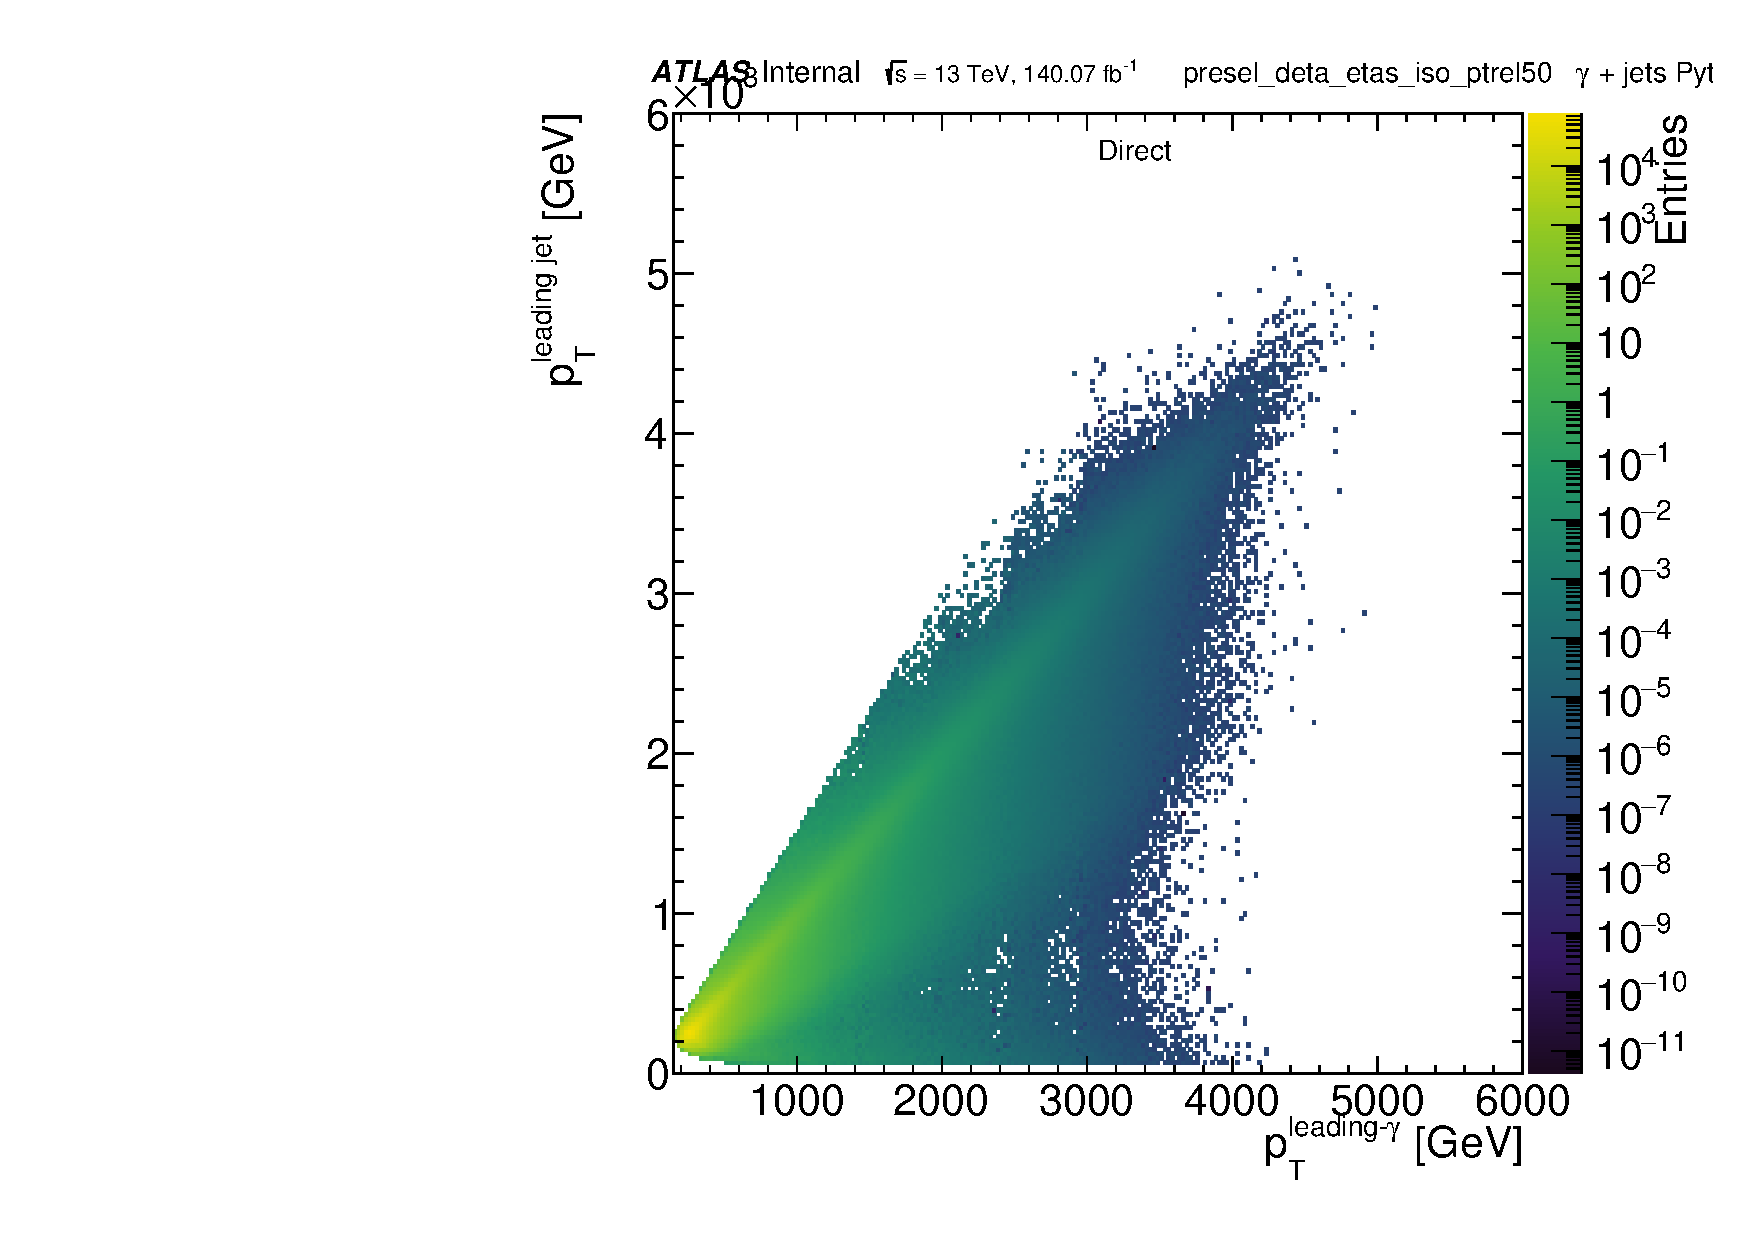
\includegraphics[width=\linewidth]{5_resonances/event_selection/jet_pt/presel_deta_etas_iso_ptrel50/bkg/2d/can2d__direct__presel_deta_etas_iso_ptrel50__ph_pt0_jet_pt0}
        \caption{\acp{DP}.}
    \end{subfigure}
    \hfill
    \begin{subfigure}[h]{0.49\linewidth}
        \centering
        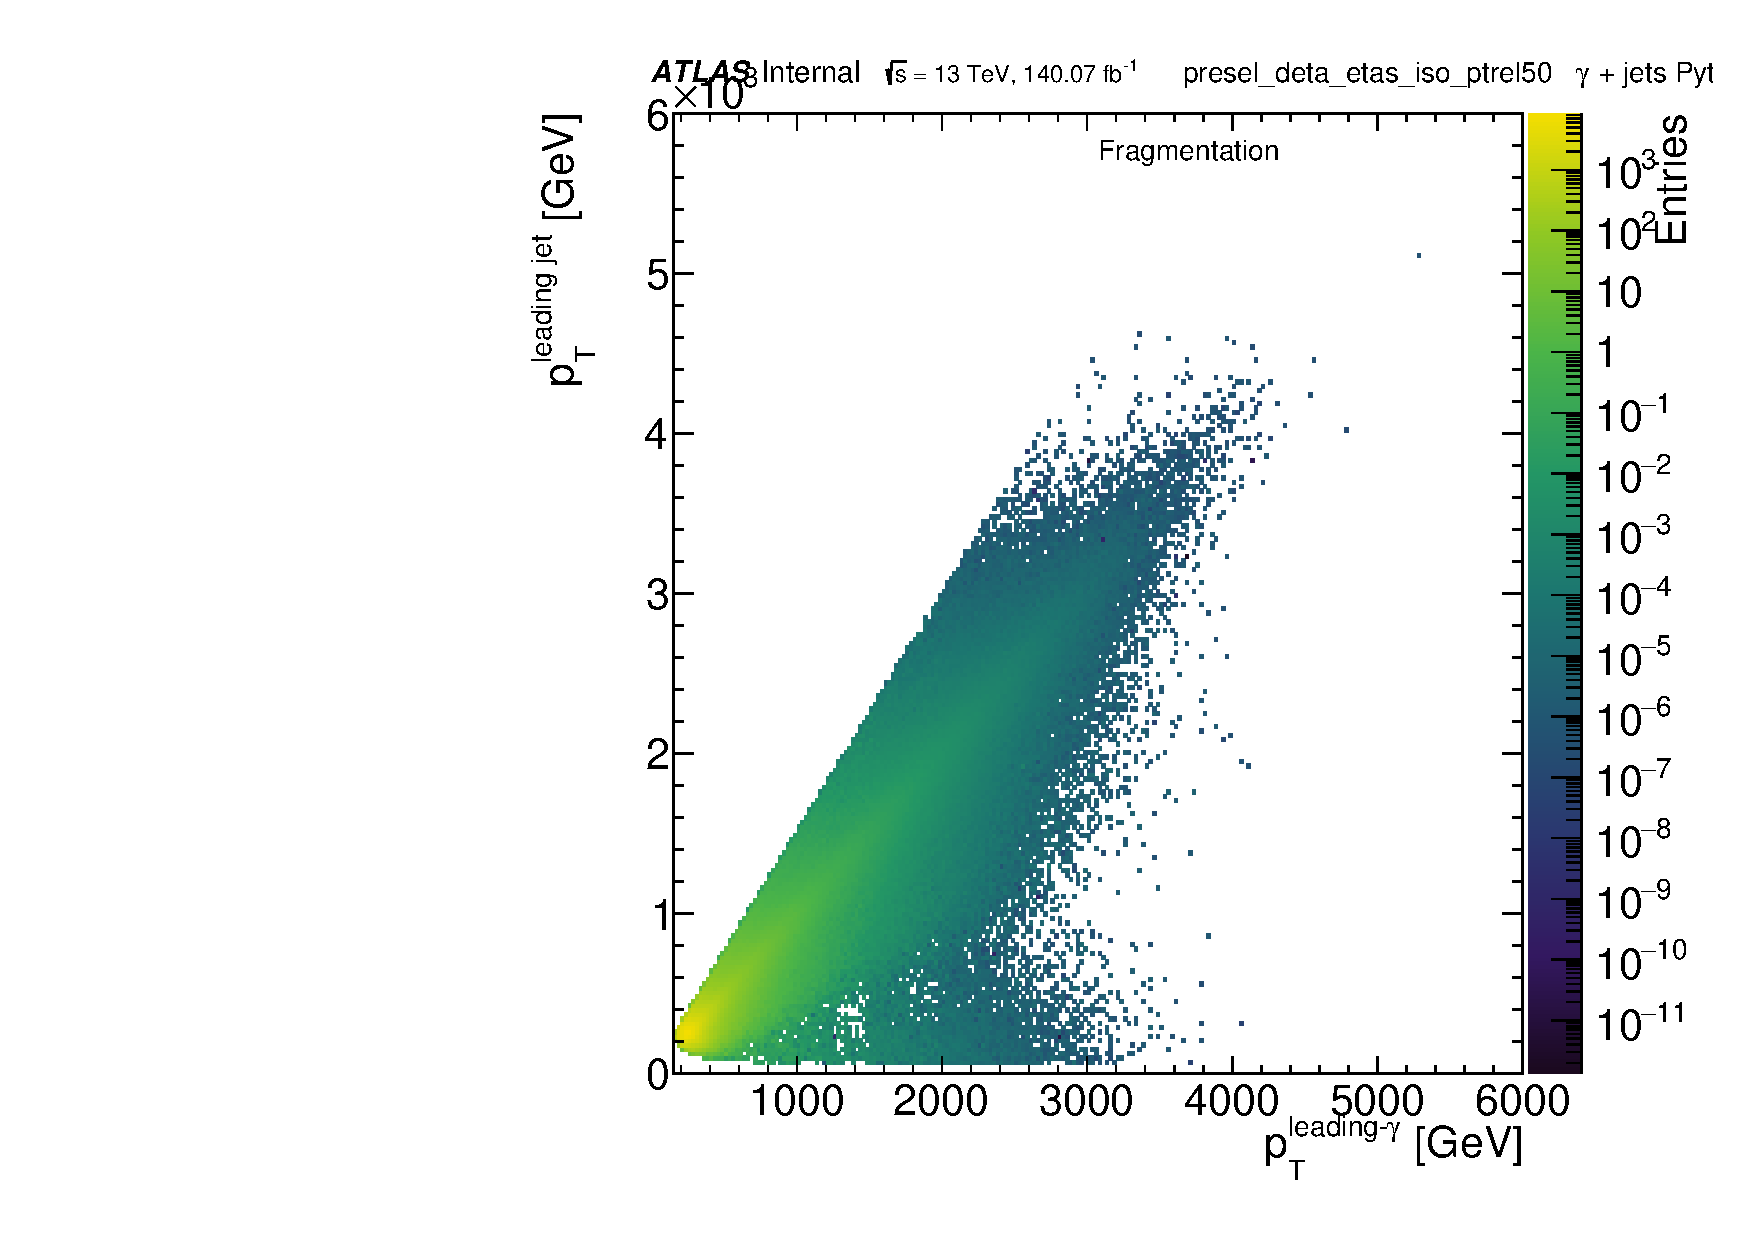
\includegraphics[width=\linewidth]{5_resonances/event_selection/jet_pt/presel_deta_etas_iso_ptrel50/bkg/2d/can2d__fragmentation__presel_deta_etas_iso_ptrel50__ph_pt0_jet_pt0}
        \caption{\acp{FP}.}
    \end{subfigure}
    \caption{Distribución bidimensional \ptgam-\ptjet para \acp{DP} y \acp{FP}, seleccionando eventos en los cuales el \pt del jet leading satisface \Eqn{\ref{eq:evt_selection:sr_opt:jet_pt:jet_pt_rel_X}} con \(X=0.5\).}
    \label{fig:evt_selection:sr_opt:jet_pt:ptgam_ptjet_X0.5}
\end{figure}



Para limpiar aún más la muestra de contribuciones de \acp{FP}, los eventos seleccionados deben satisfacer:
\begin{equation}
    \label{eq:evt_selection:sr_opt:jet_pt:jet_pt_rel_X}
    \frac{\ptjet - \ptgam}{\ptgam} < X, \qquad X \in [0, 1]
\end{equation}
donde \(X\) es la fracción de \ptgam permitida para el jet, definiendo así un valor superior de \ptjet para un \ptgam dado. El valor óptimo es \(X=0.5\), en el que la eficiencia de la señal es muy alta, mientras que el fondo rechazado consiste únicamente en eventos de \acp{FP}.

En la \Fig{\ref{fig:evt_selection:sr_opt:jet_pt:ptgam_ptjet_X0.5}} se muestra la distribución de fondo \ptgam vs \ptjet por separado para \acp{DP} y \acp{FP}, donde se observa que la gran mayoría de los eventos eliminados corresponden a \acp{FP}. La misma distribución para diferentes señales de \ac{EQ} se muestra en \Fig{\ref{fig:evt_selection:sr_opt:jet_pt:ptgam_ptjet_signals}} con eficiencias superiores al 95\%. La eficiencia de corte para el fondo y algunas señales \qstar se presenta en la \Tab{\ref{tab:evt_selection:sr_opt:jet_pt:efficiency_selection}}, donde se aprecia el poco efecto que tiene dicho corte en las señales.


\begin{figure}[ht!]
    \centering
    \begin{subfigure}[h]{0.32\linewidth}
        \centering
        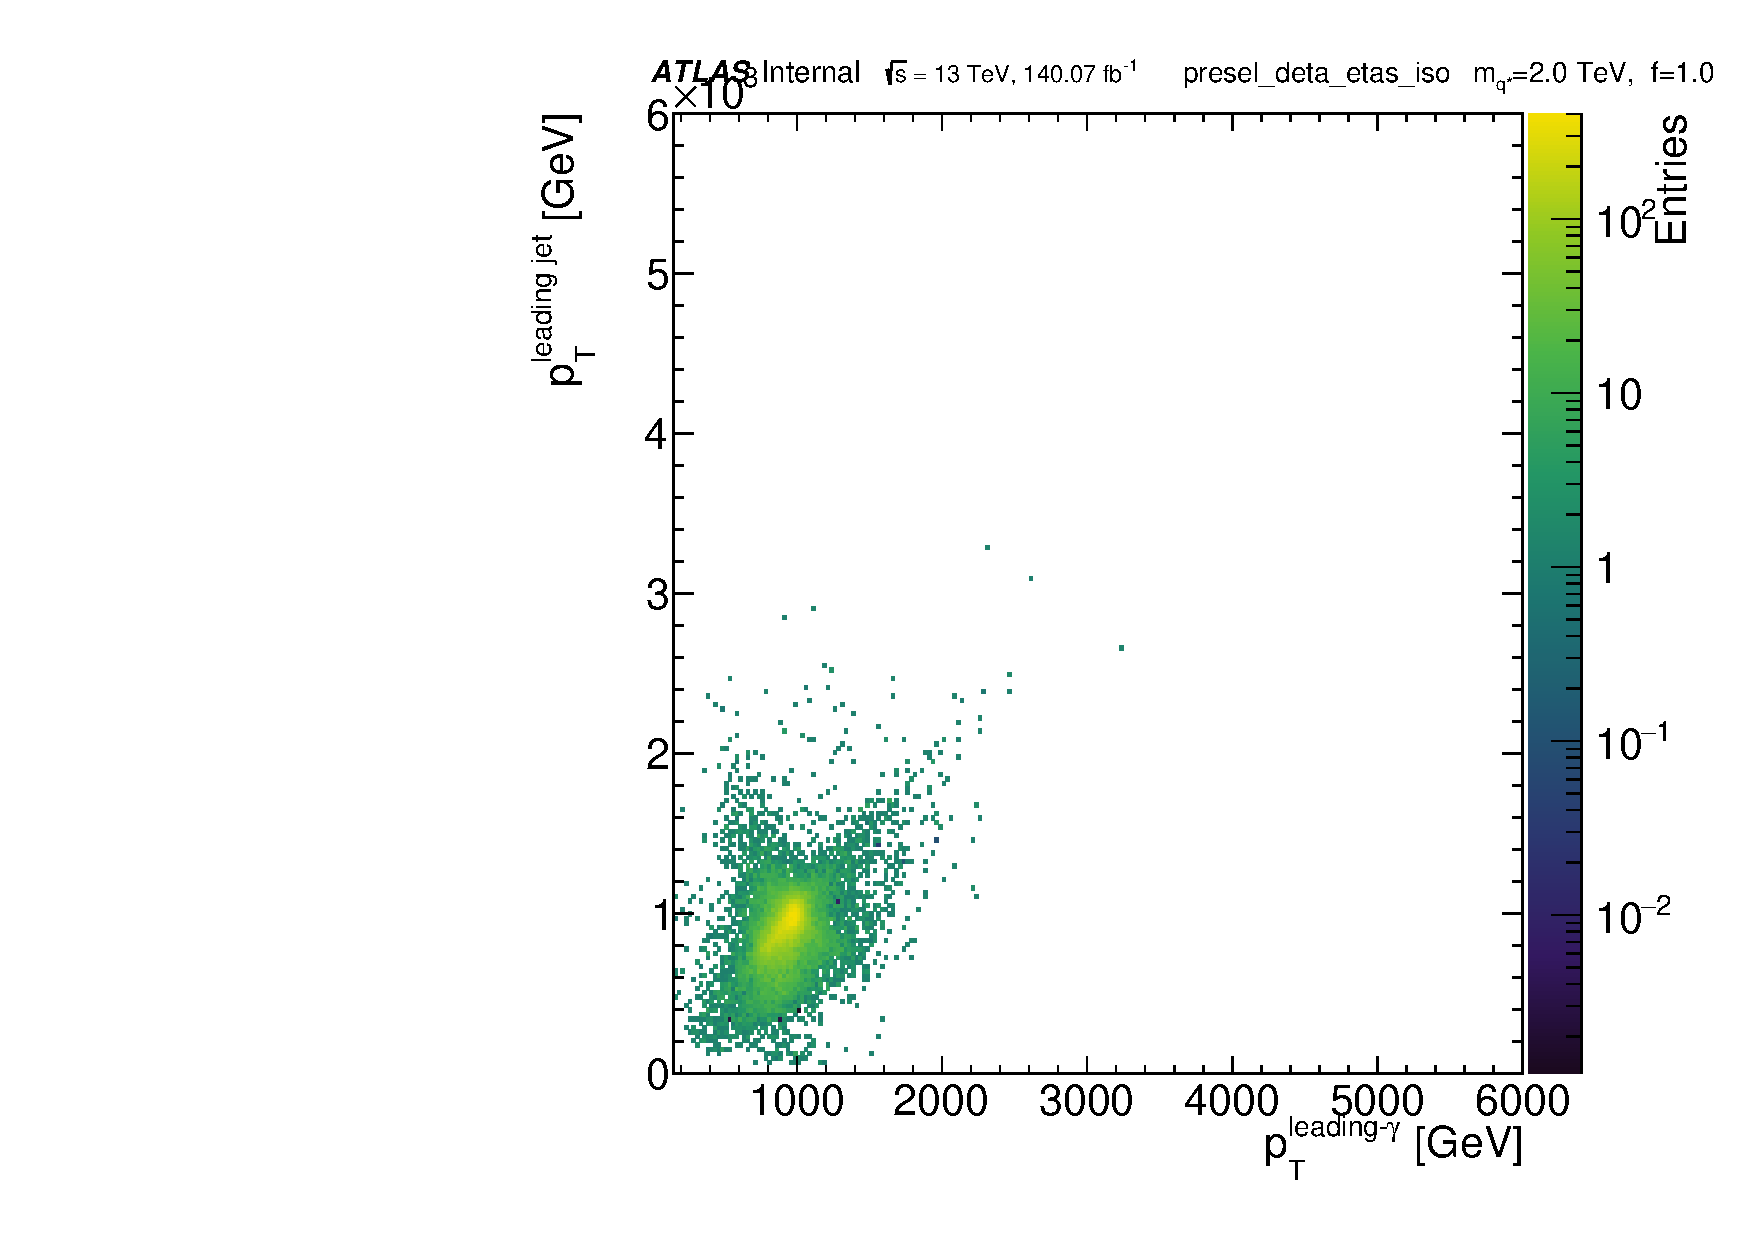
\includegraphics[width=\linewidth]{5_resonances/event_selection/jet_pt/presel_deta_etas_iso/sig/2d/can2d__qStar_f1p00_M2000__presel_deta_etas_iso__ph_pt0_jet_pt0}
        \caption{\(\mq=2000~\gev\).}
    \end{subfigure}
    \hfill
    \begin{subfigure}[h]{0.32\linewidth}
        \centering
        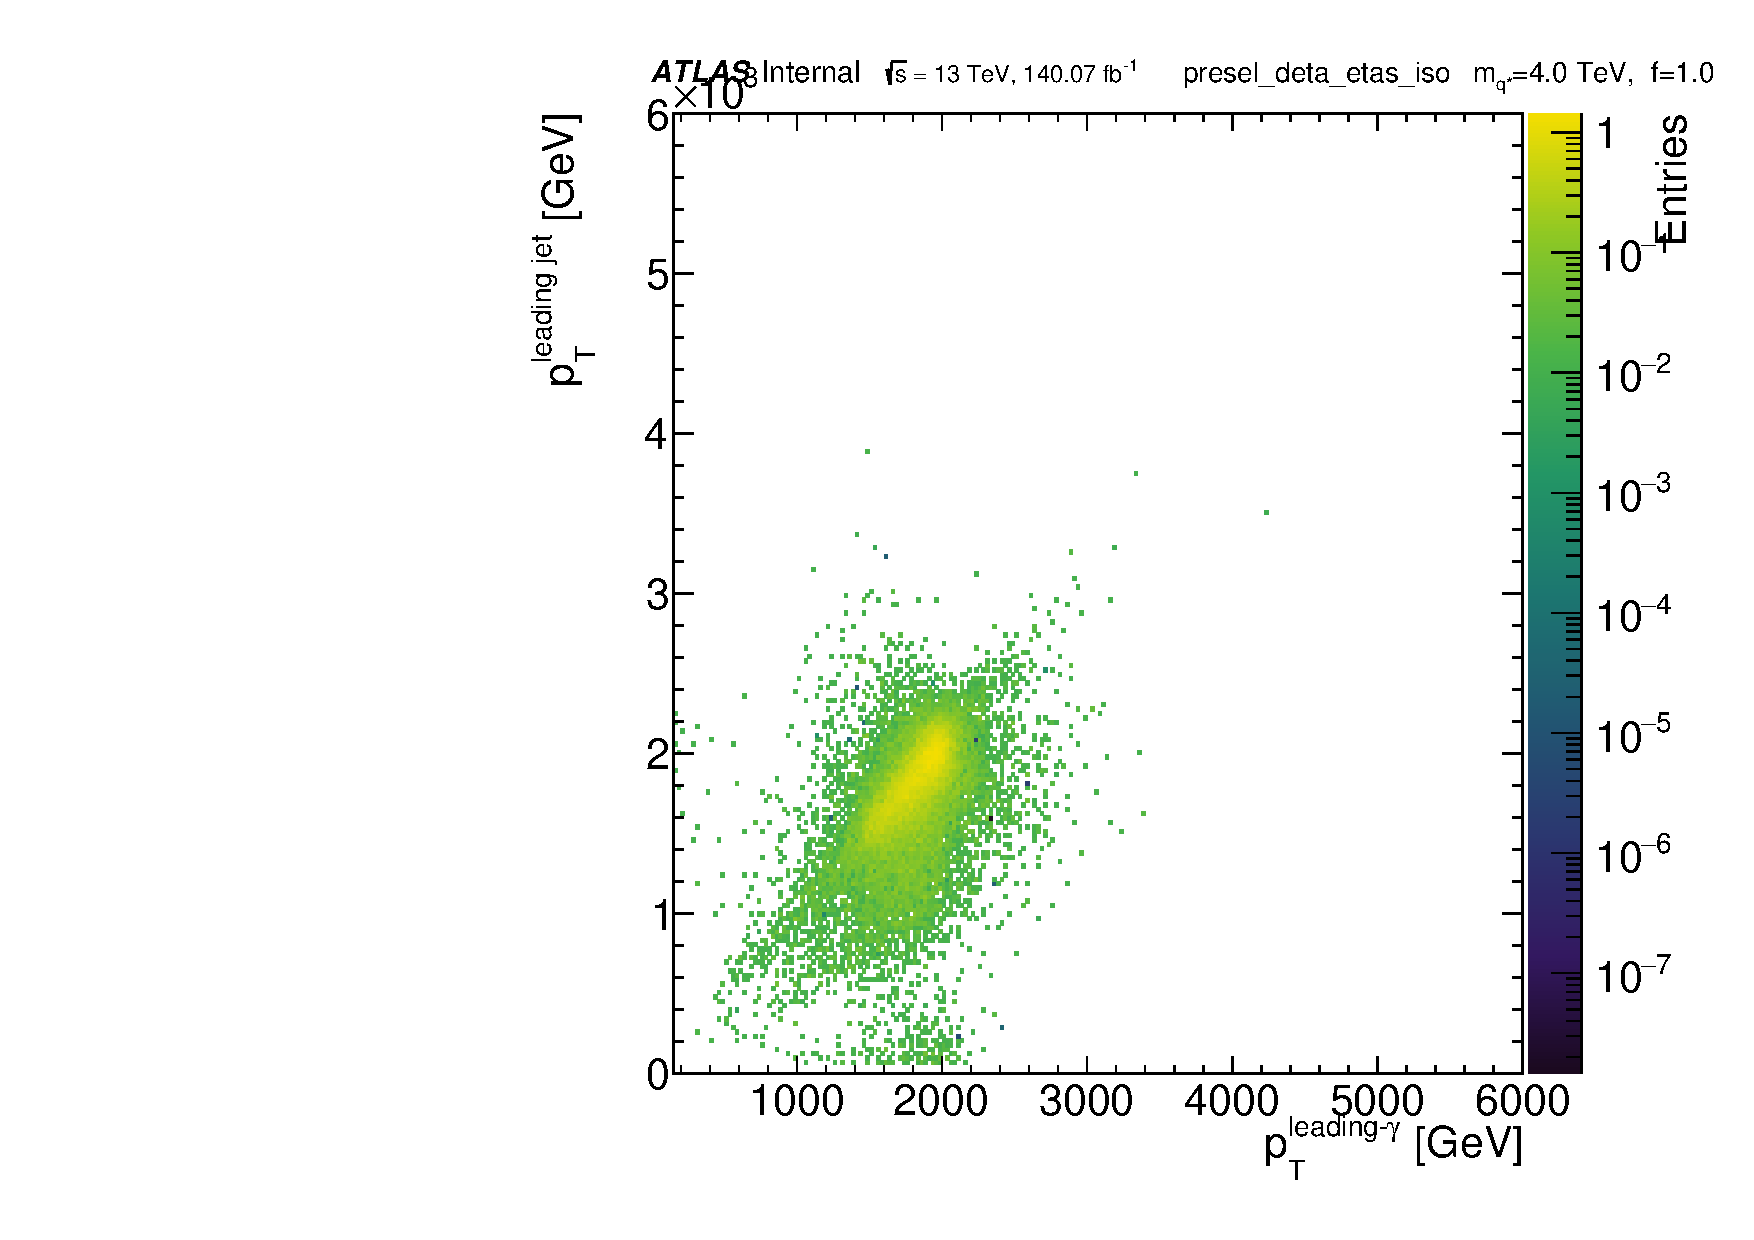
\includegraphics[width=\linewidth]{5_resonances/event_selection/jet_pt/presel_deta_etas_iso/sig/2d/can2d__qStar_f1p00_M4000__presel_deta_etas_iso__ph_pt0_jet_pt0}
        \caption{\(\mq=4000~\gev\).}
    \end{subfigure}
    \hfill
    \begin{subfigure}[h]{0.32\linewidth}
        \centering
        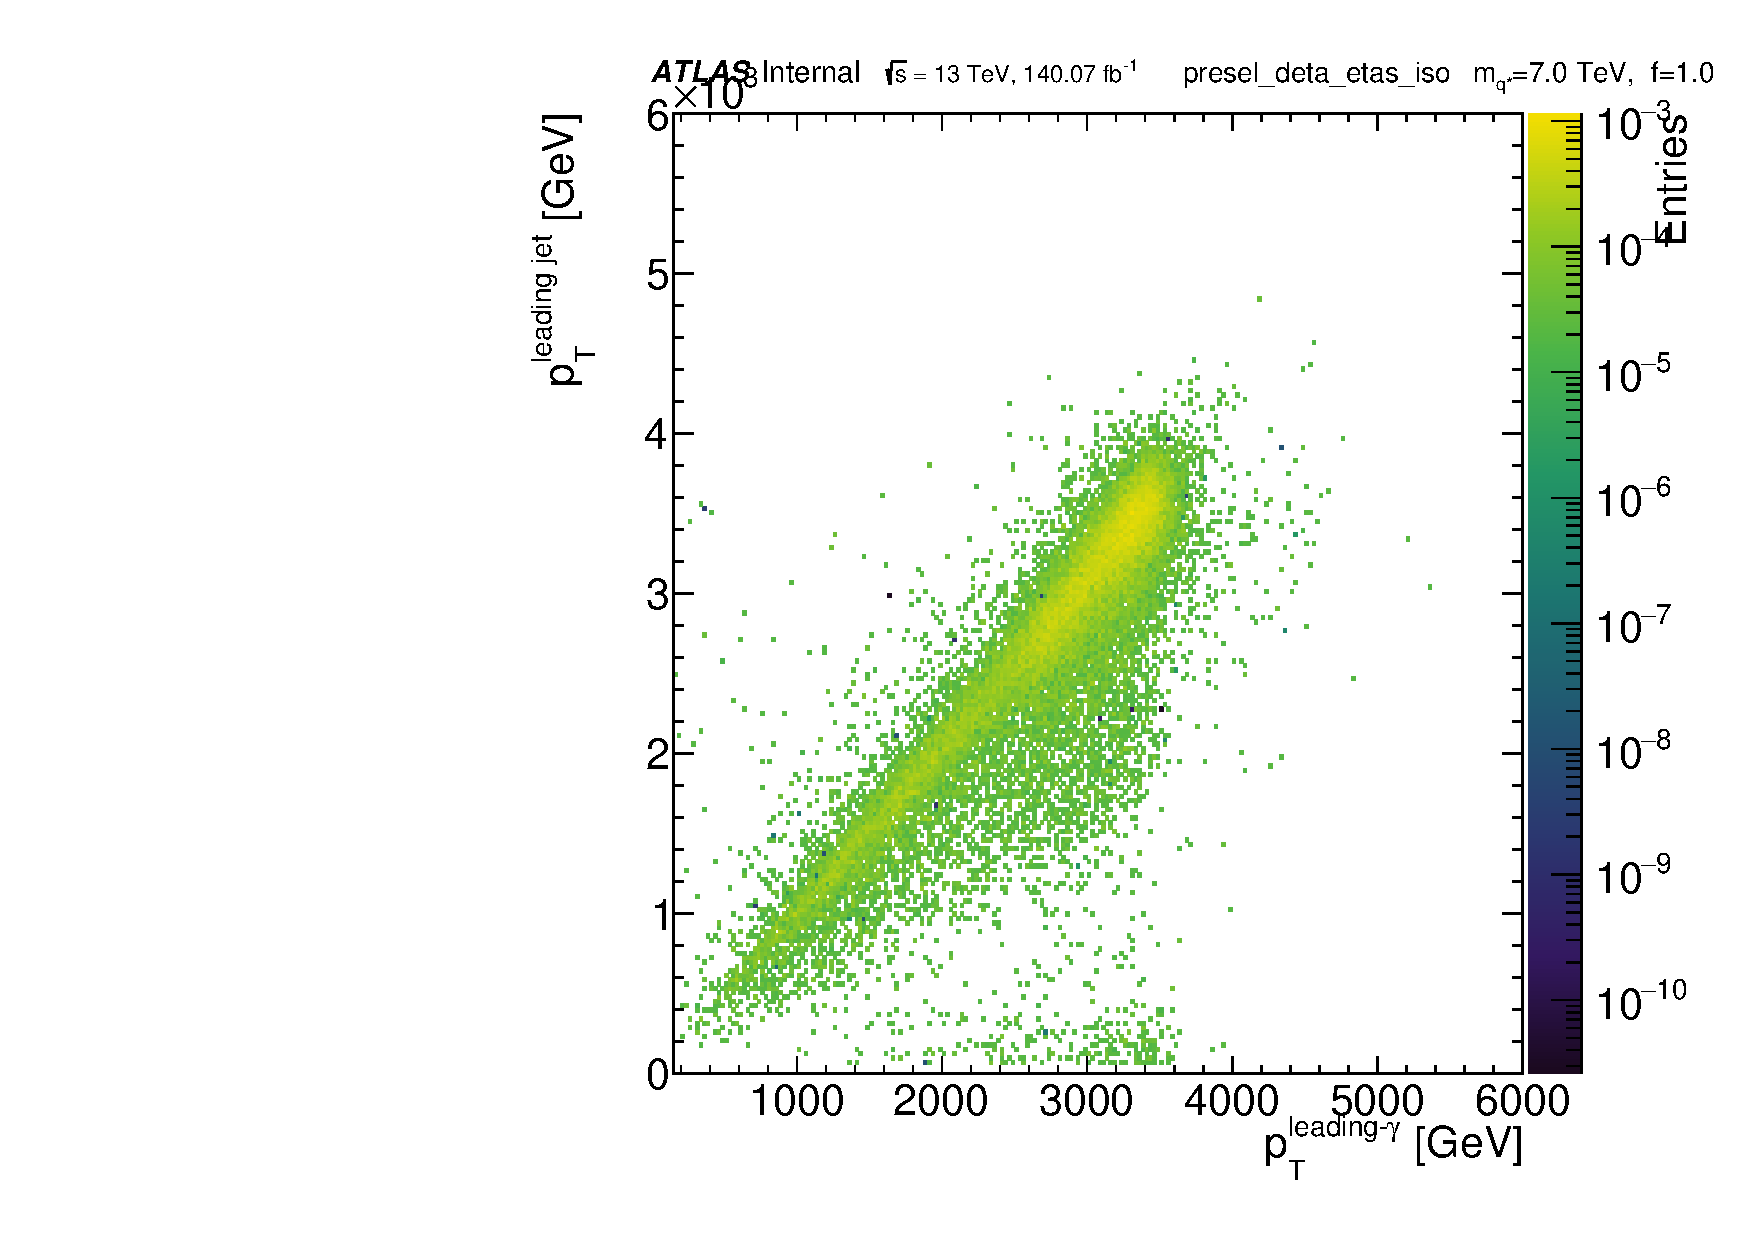
\includegraphics[width=\linewidth]{5_resonances/event_selection/jet_pt/presel_deta_etas_iso/sig/2d/can2d__qStar_f1p00_M7000__presel_deta_etas_iso__ph_pt0_jet_pt0}
        \caption{\(\mq=7000~\gev\).}
    \end{subfigure}\\
    \begin{subfigure}[h]{0.32\linewidth}
        \centering
        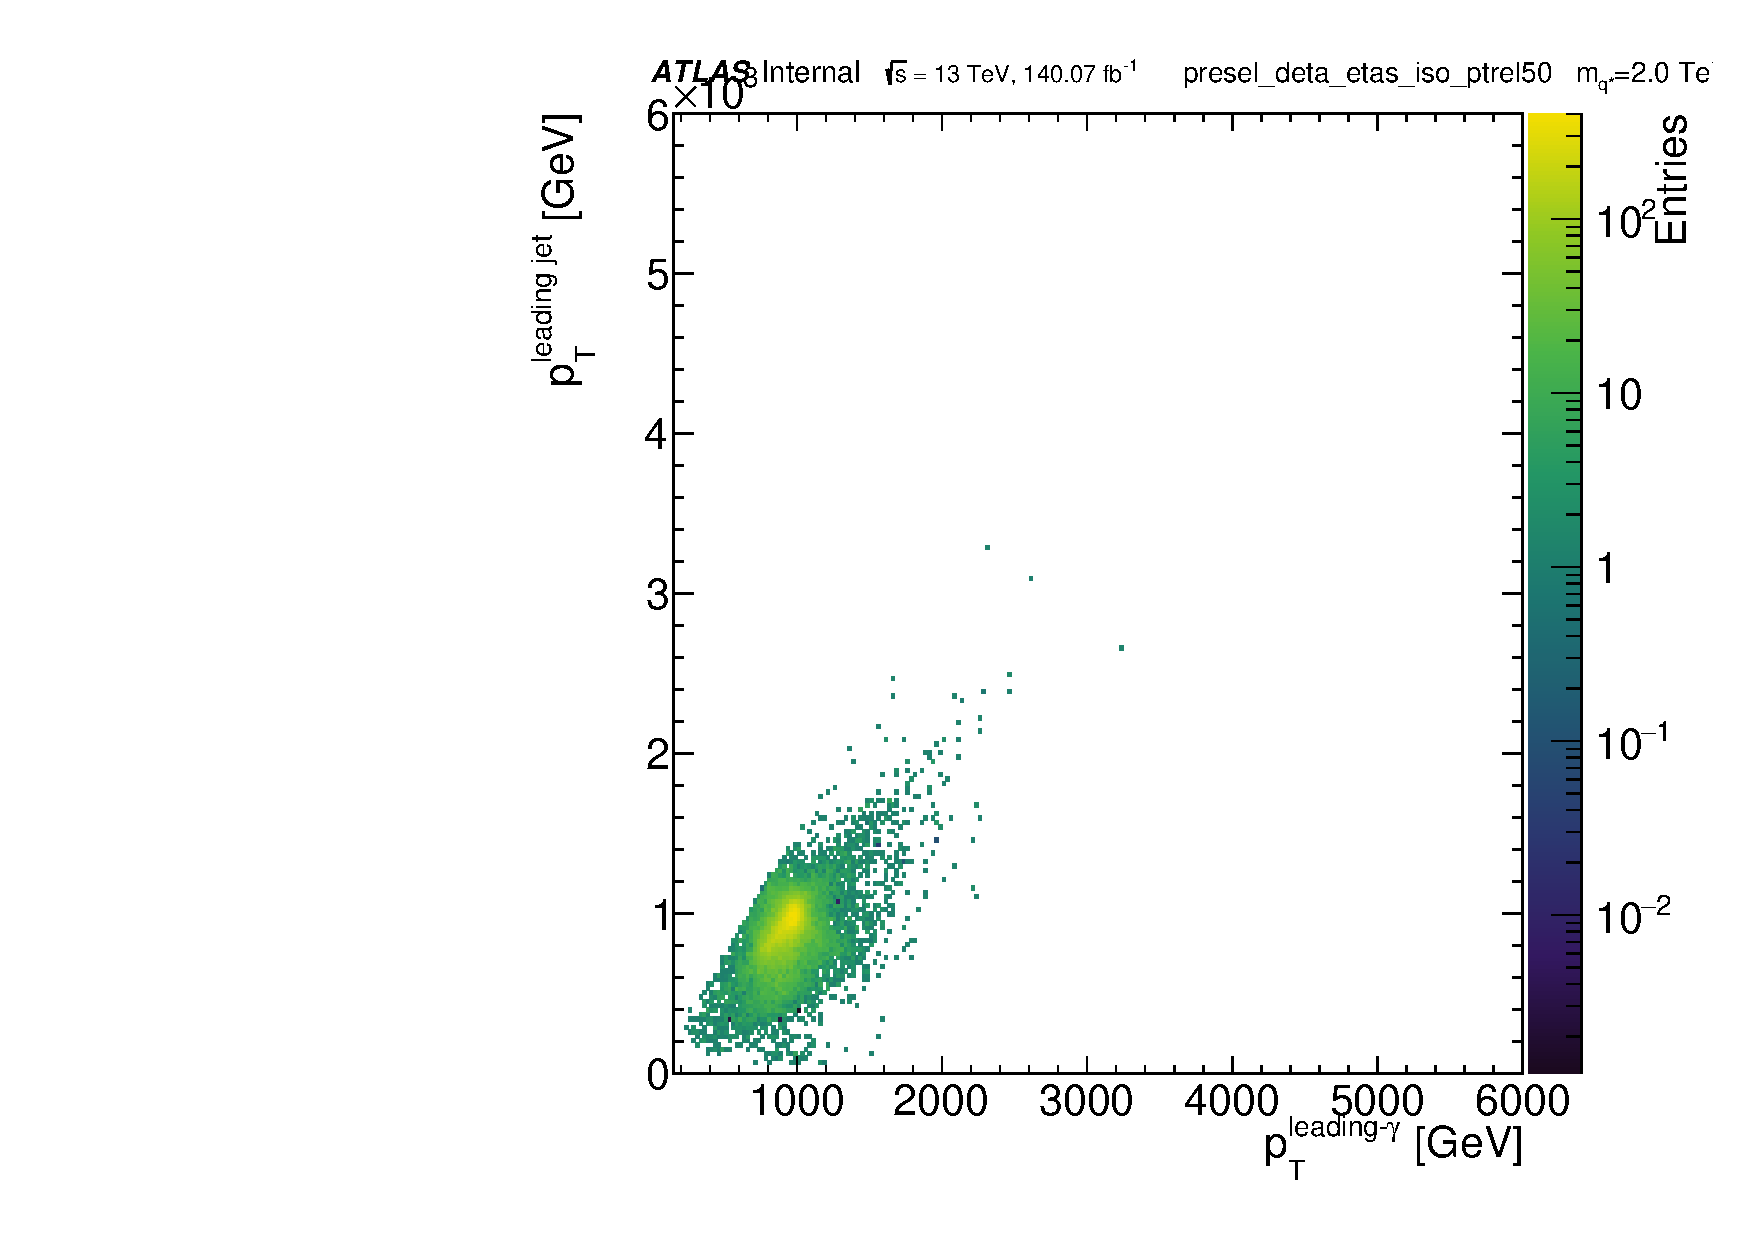
\includegraphics[width=\linewidth]{5_resonances/event_selection/jet_pt/presel_deta_etas_iso_ptrel50/sig/2d/can2d__qStar_f1p00_M2000__presel_deta_etas_iso_ptrel50__ph_pt0_jet_pt0}
        \caption{\(\mq=2000~\gev\), con el corte de \ptjet aplicado.}
    \end{subfigure}
    \hfill
    \begin{subfigure}[h]{0.32\linewidth}
        \centering
        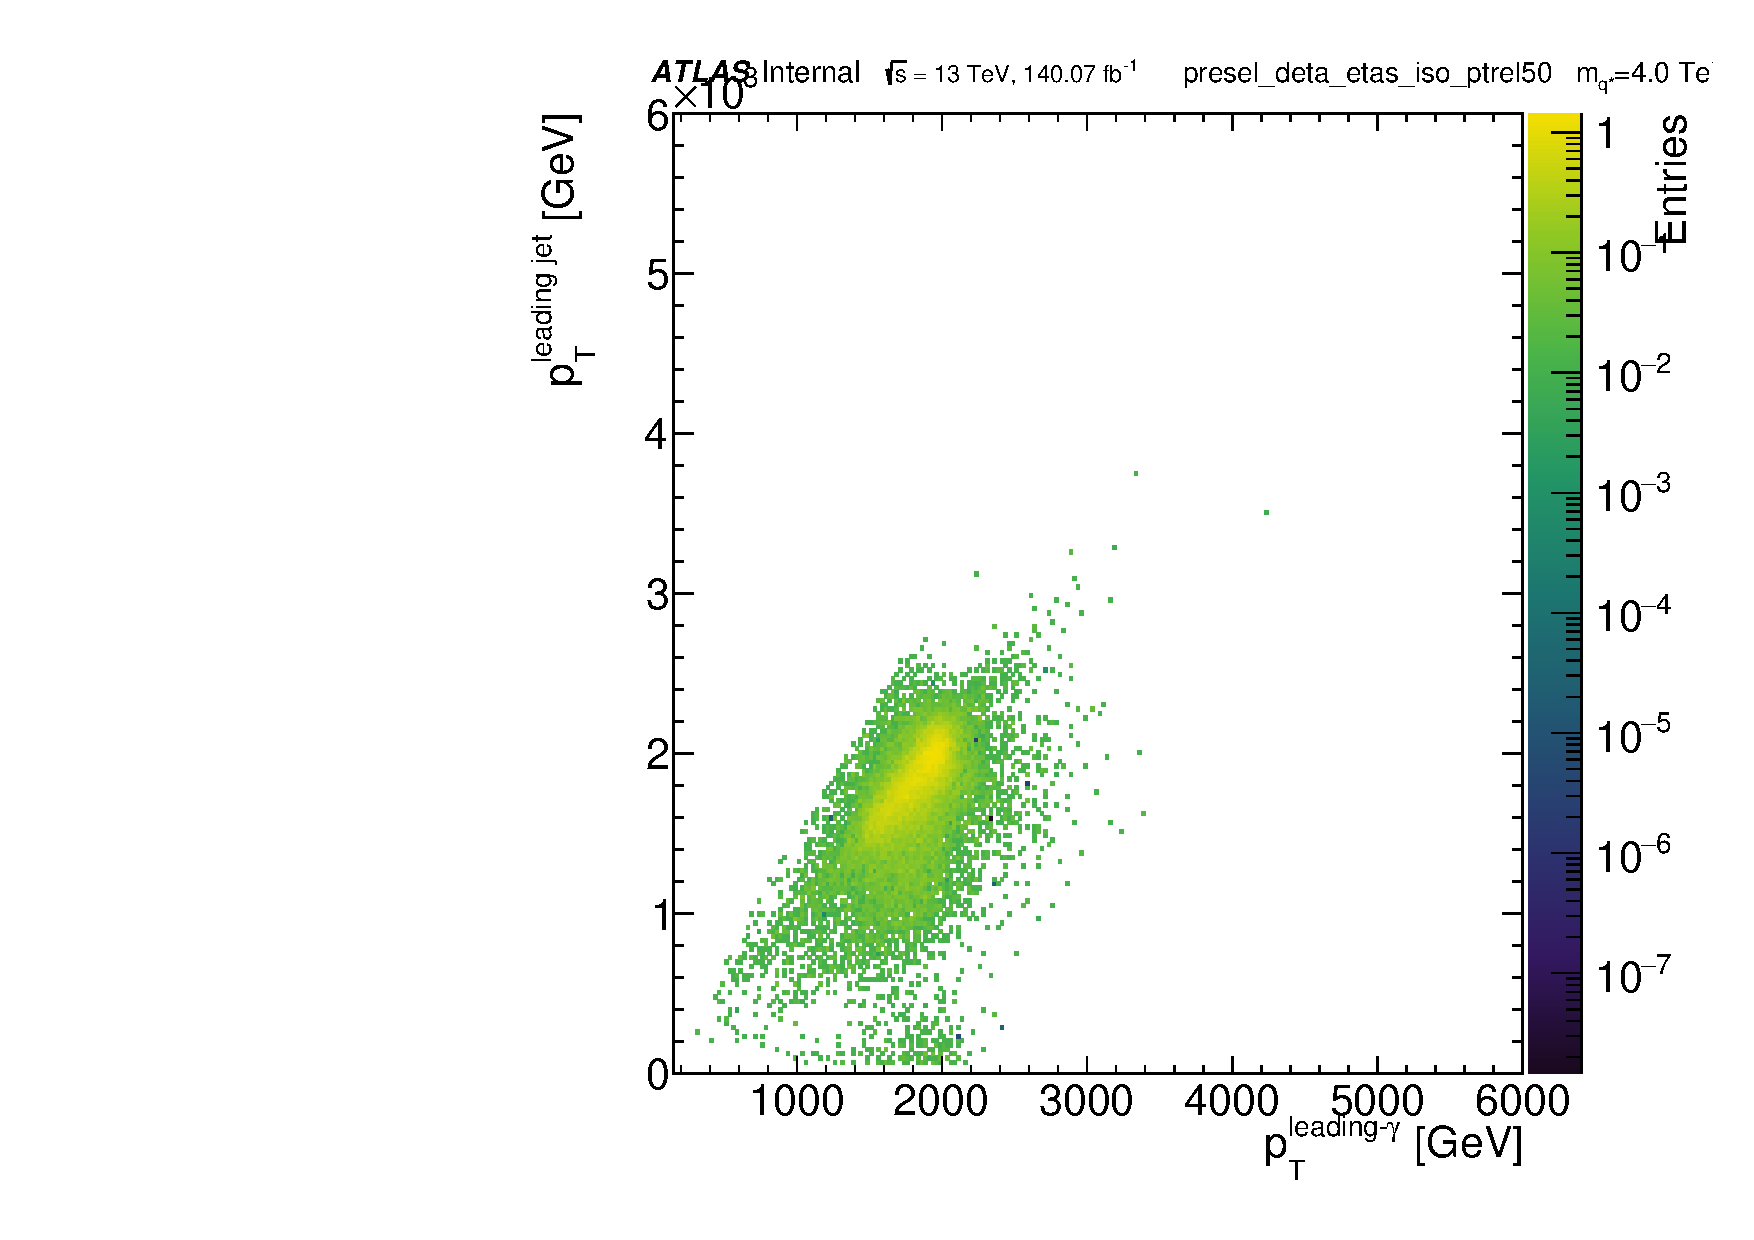
\includegraphics[width=\linewidth]{5_resonances/event_selection/jet_pt/presel_deta_etas_iso_ptrel50/sig/2d/can2d__qStar_f1p00_M4000__presel_deta_etas_iso_ptrel50__ph_pt0_jet_pt0}
        \caption{\(\mq=4000~\gev\), con el corte de \ptjet aplicado.}
    \end{subfigure}
    \hfill
    \begin{subfigure}[h]{0.32\linewidth}
        \centering
        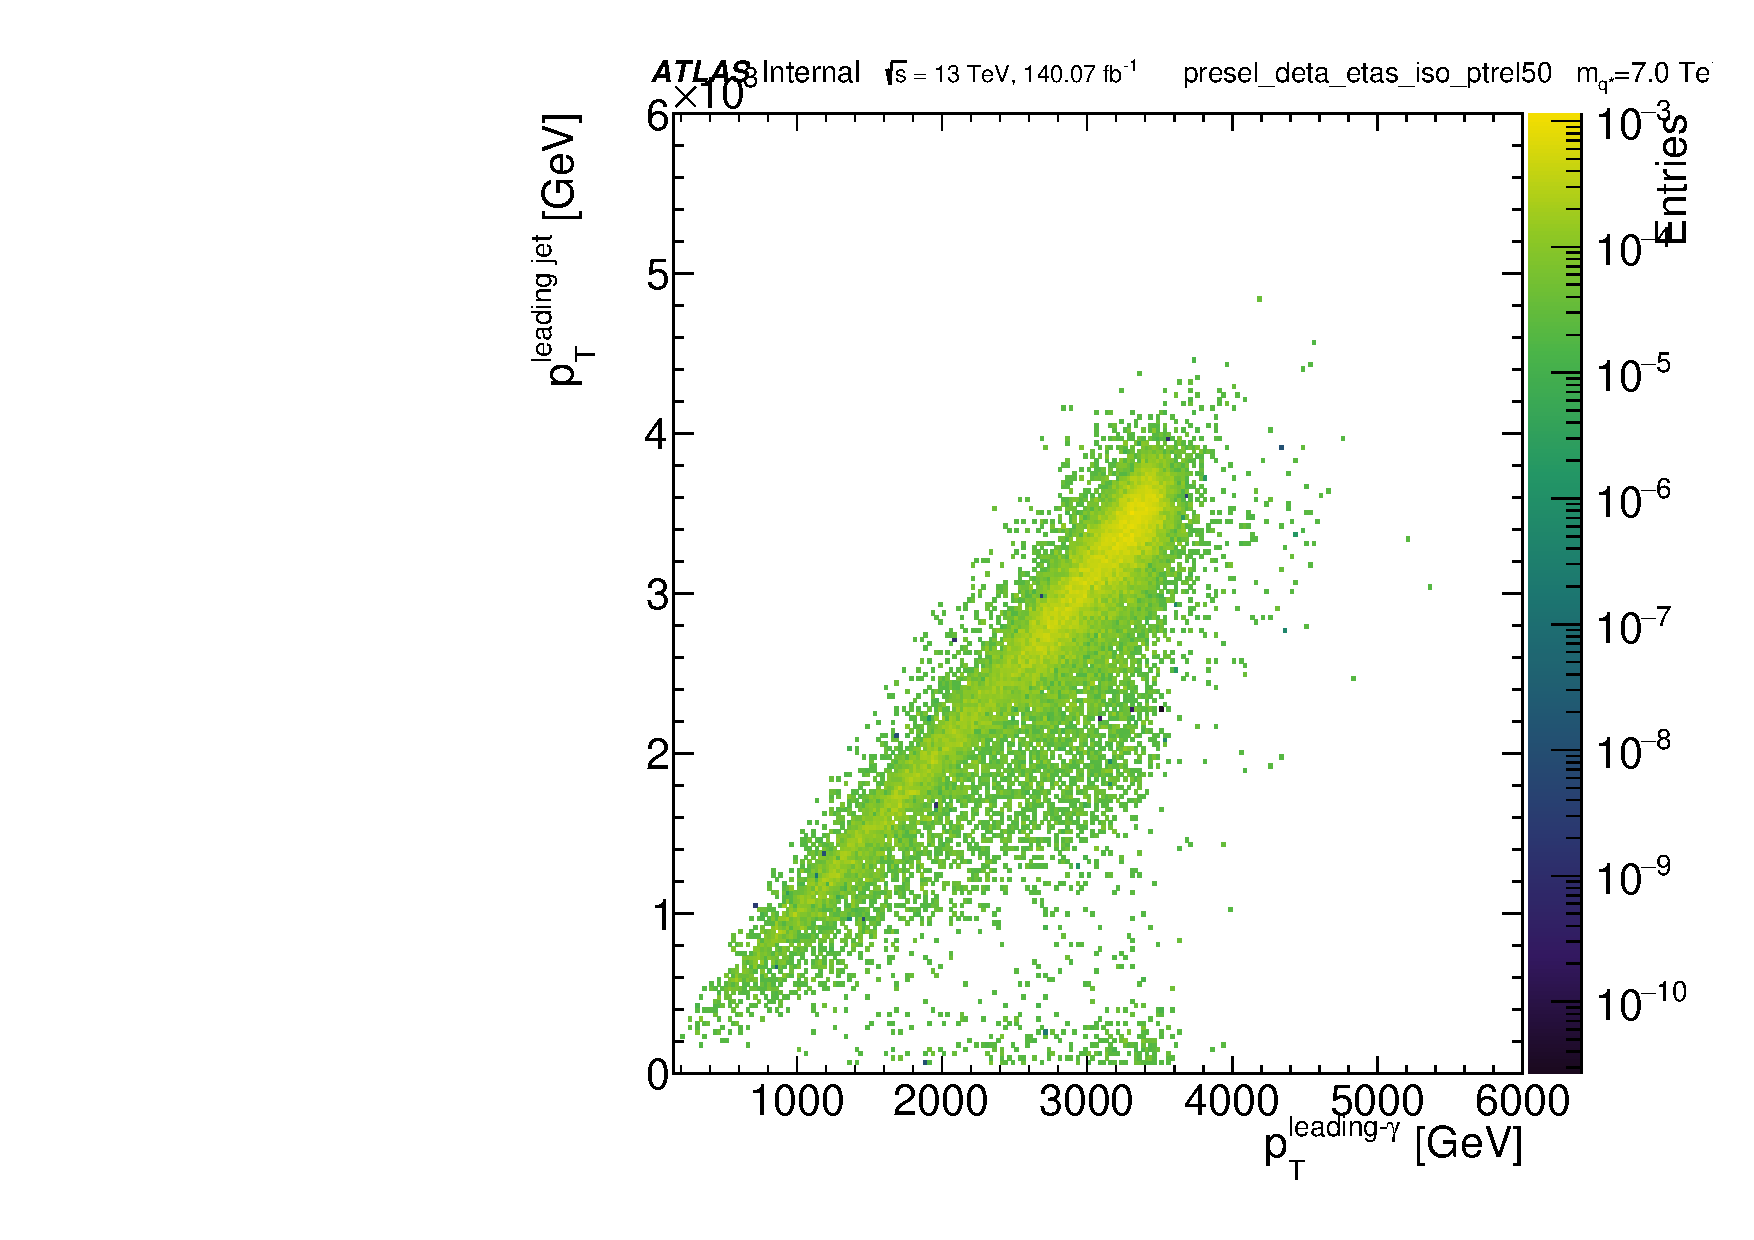
\includegraphics[width=\linewidth]{5_resonances/event_selection/jet_pt/presel_deta_etas_iso_ptrel50/sig/2d/can2d__qStar_f1p00_M7000__presel_deta_etas_iso_ptrel50__ph_pt0_jet_pt0}
        \caption{\(\mq=7000~\gev\), con el corte de \ptjet aplicado.}
    \end{subfigure}\\
    \caption{Distribución bidimensional \ptgam-\ptjet para diferentes señales de \qstar con \(f=1.0\), seleccionando jets de acuerdo a la \Eqn{\ref{eq:evt_selection:sr_opt:jet_pt:jet_pt_rel_X}} con \(X=0.5\). Las primeras tres figuras muestran las distribuciones sin la aplicación del corte de \ptjet, mientras que las tres de abajo lo contienen.}
    \label{fig:evt_selection:sr_opt:jet_pt:ptgam_ptjet_signals}
\end{figure}



\begin{table}[ht!]
    \centering
    \caption{Eficiencias del corte en \ptjet del fondo y de distintas señales de \qstar.}
    \begin{tabular}{lc}
        \toprule
        & \(\varepsilon_{\text{rel}}\) \\
        \midrule
        \gammajet                      & $0.8827$ \\
        \(\mq=2000~\gev\),  \(f=1.00\) & $0.9707$ \\
        \(\mq=4000~\gev\),  \(f=1.00\) & $0.9918$ \\
        \(\mq=7000~\gev\),  \(f=1.00\) & $0.9942$ \\
        \bottomrule
    \end{tabular}
    \label{tab:evt_selection:sr_opt:jet_pt:efficiency_selection}
\end{table}



La variable más afectada por este corte es, como era de esperar, \ptjet. Esta distribución se muestra en la \Fig{\ref{fig:evt_selection:sr_opt:jet_pt:jet_pt}} antes y después de aplicar el corte. Se observa cómo la contribución de los eventos \acp{FP} disminuye drásticamente haciendo que la distribución \ptjet sea mucho más suave. Además, dado que el observable de interés es \myj, se presenta una comparación de esta distribución en la \Fig{\ref{fig:evt_selection:sr_opt:jet_pt:phjet_m}} para evaluar los cambios en el espectro. La aplicación de este corte particular sobre \ptjet tiene un efecto despreciable sobre la distribución final de \myj. Se observan diferencias muy pequeñas pero con un \myj muy bajo. Esto se debe a la asimetría en \pt que tenían el jet y el fotón (\(\ptjet \gg \ptgam\)).

En la selección final, se aplica el corte \((\ptjet - \ptgam) / \ptgam < 0.5\).

\begin{figure}[ht!]
    \centering
    \begin{subfigure}[h]{0.32\linewidth}
        \centering
        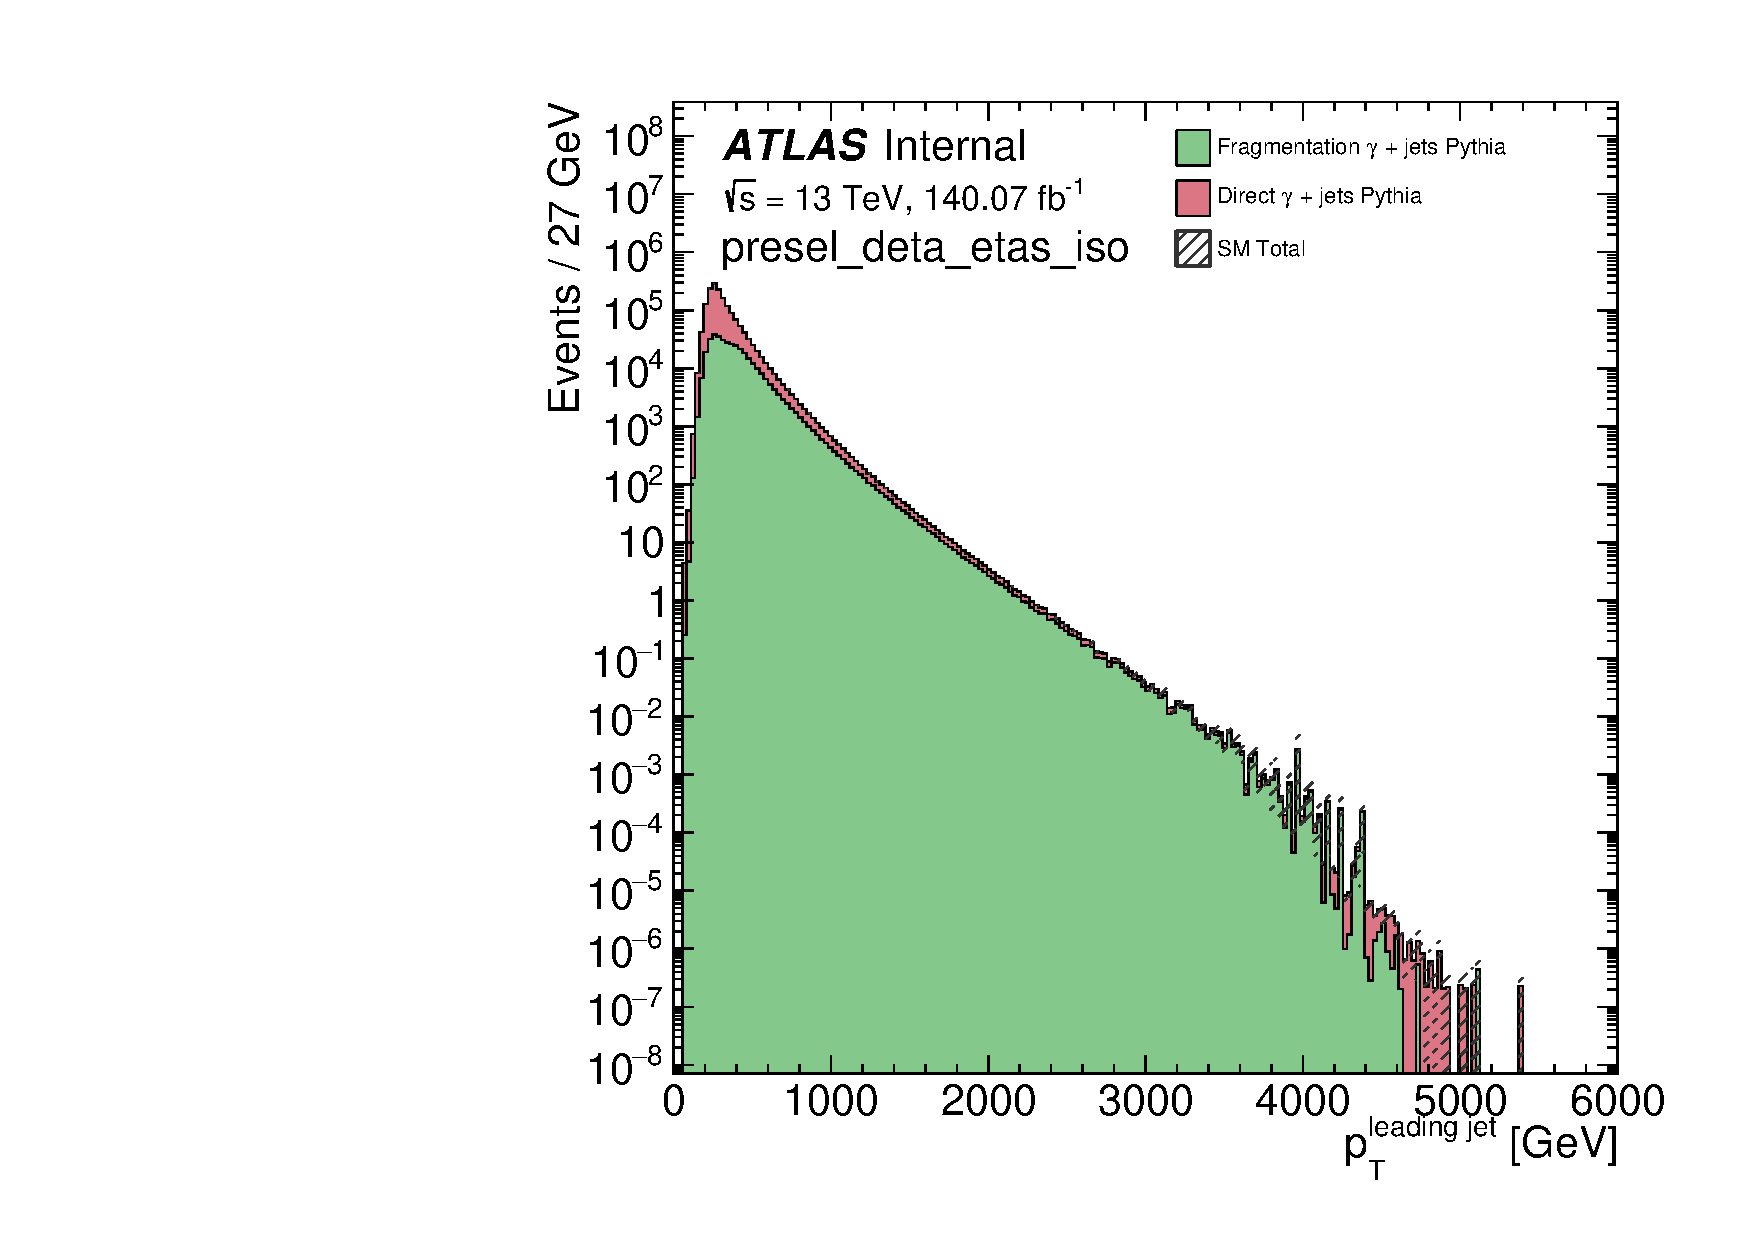
\includegraphics[width=\linewidth]{5_resonances/event_selection/jet_pt/presel_deta_etas_iso/bkg/1d/no_normalized/can__photonjet_Pythia__presel_deta_etas_iso__jet_pt0__Run2}
        \caption{Antes del corte en \ptjet.}
    \end{subfigure}
    \hfill
    \begin{subfigure}[h]{0.32\linewidth}
        \centering
        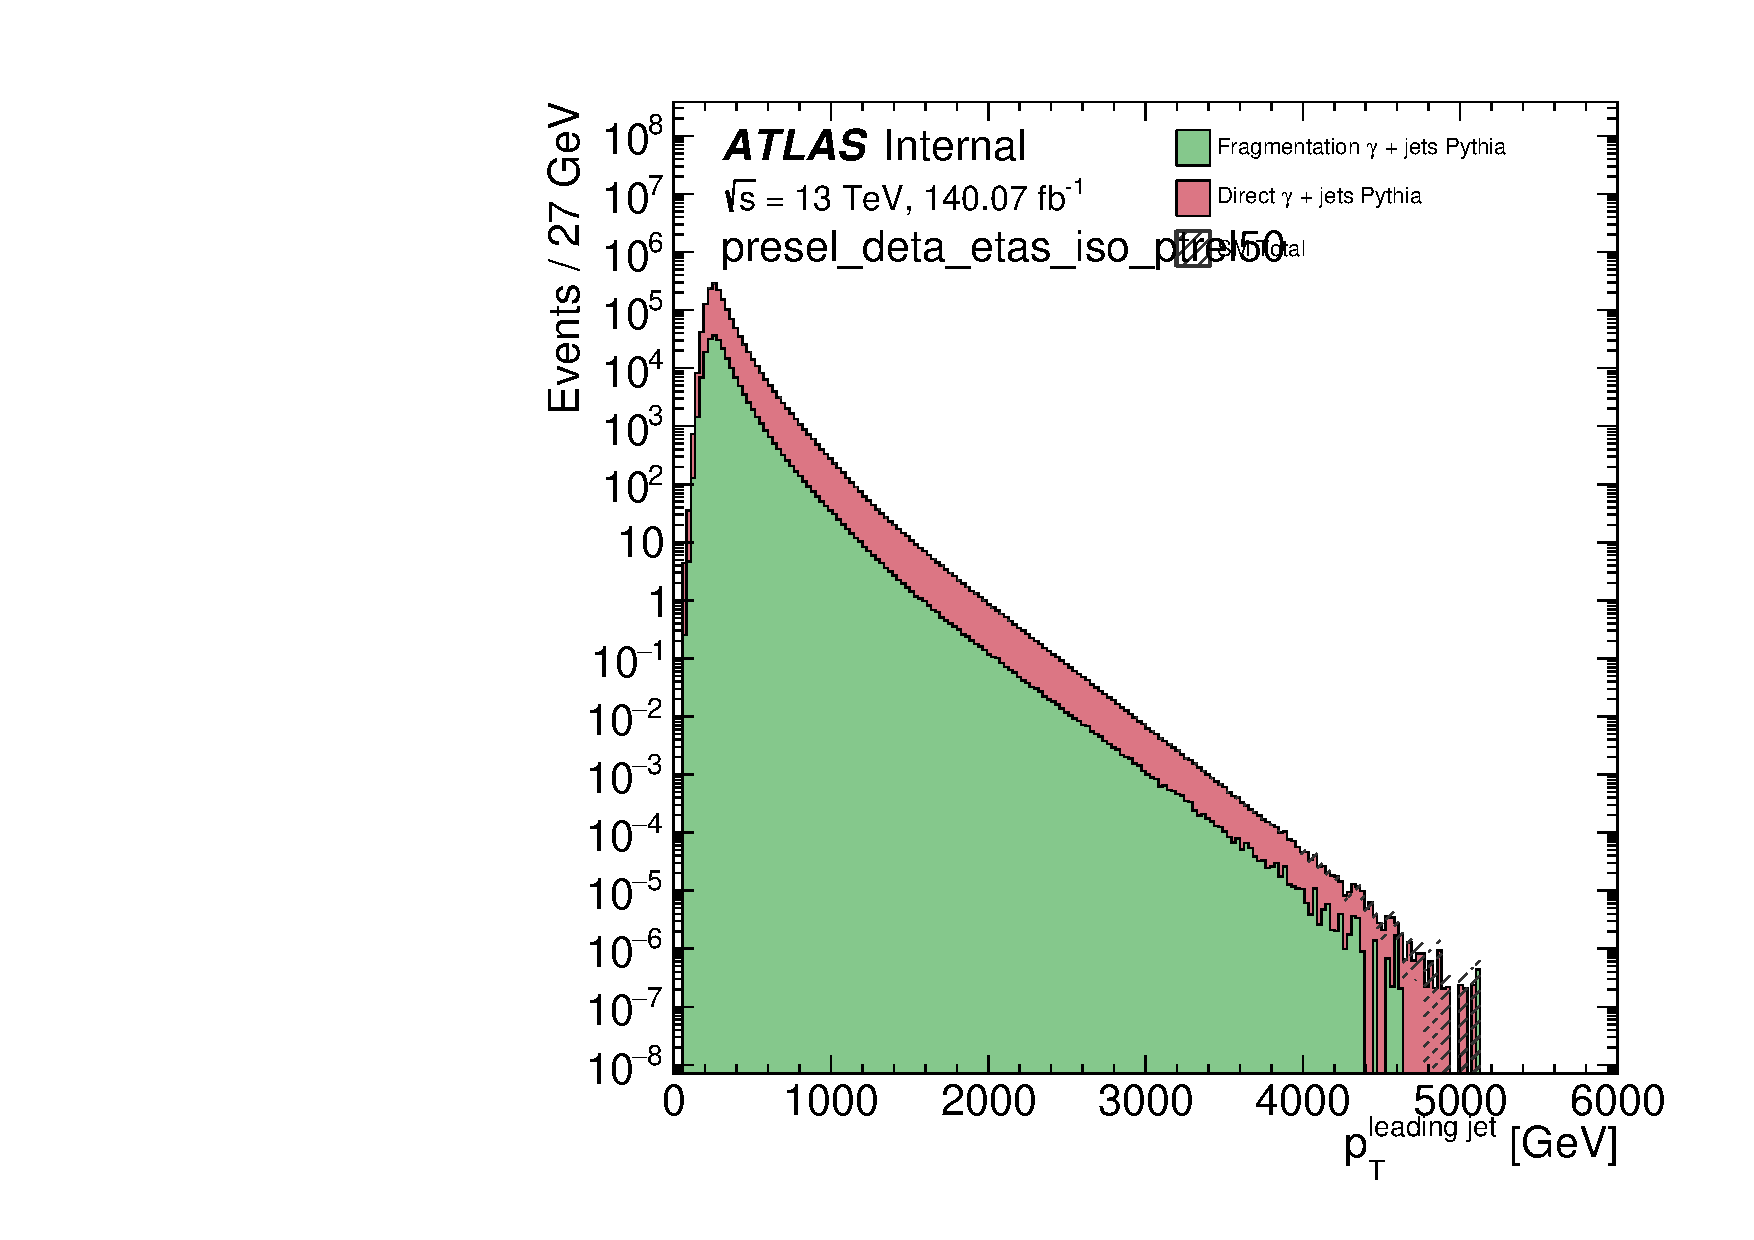
\includegraphics[width=\linewidth]{5_resonances/event_selection/jet_pt/presel_deta_etas_iso_ptrel50/bkg/1d/no_normalized/can__photonjet_Pythia__presel_deta_etas_iso_ptrel50__jet_pt0__Run2}
        \caption{Luego del corte en \ptjet.}
    \end{subfigure}
    \hfill
    \begin{subfigure}[h]{0.32\linewidth}
        \centering
        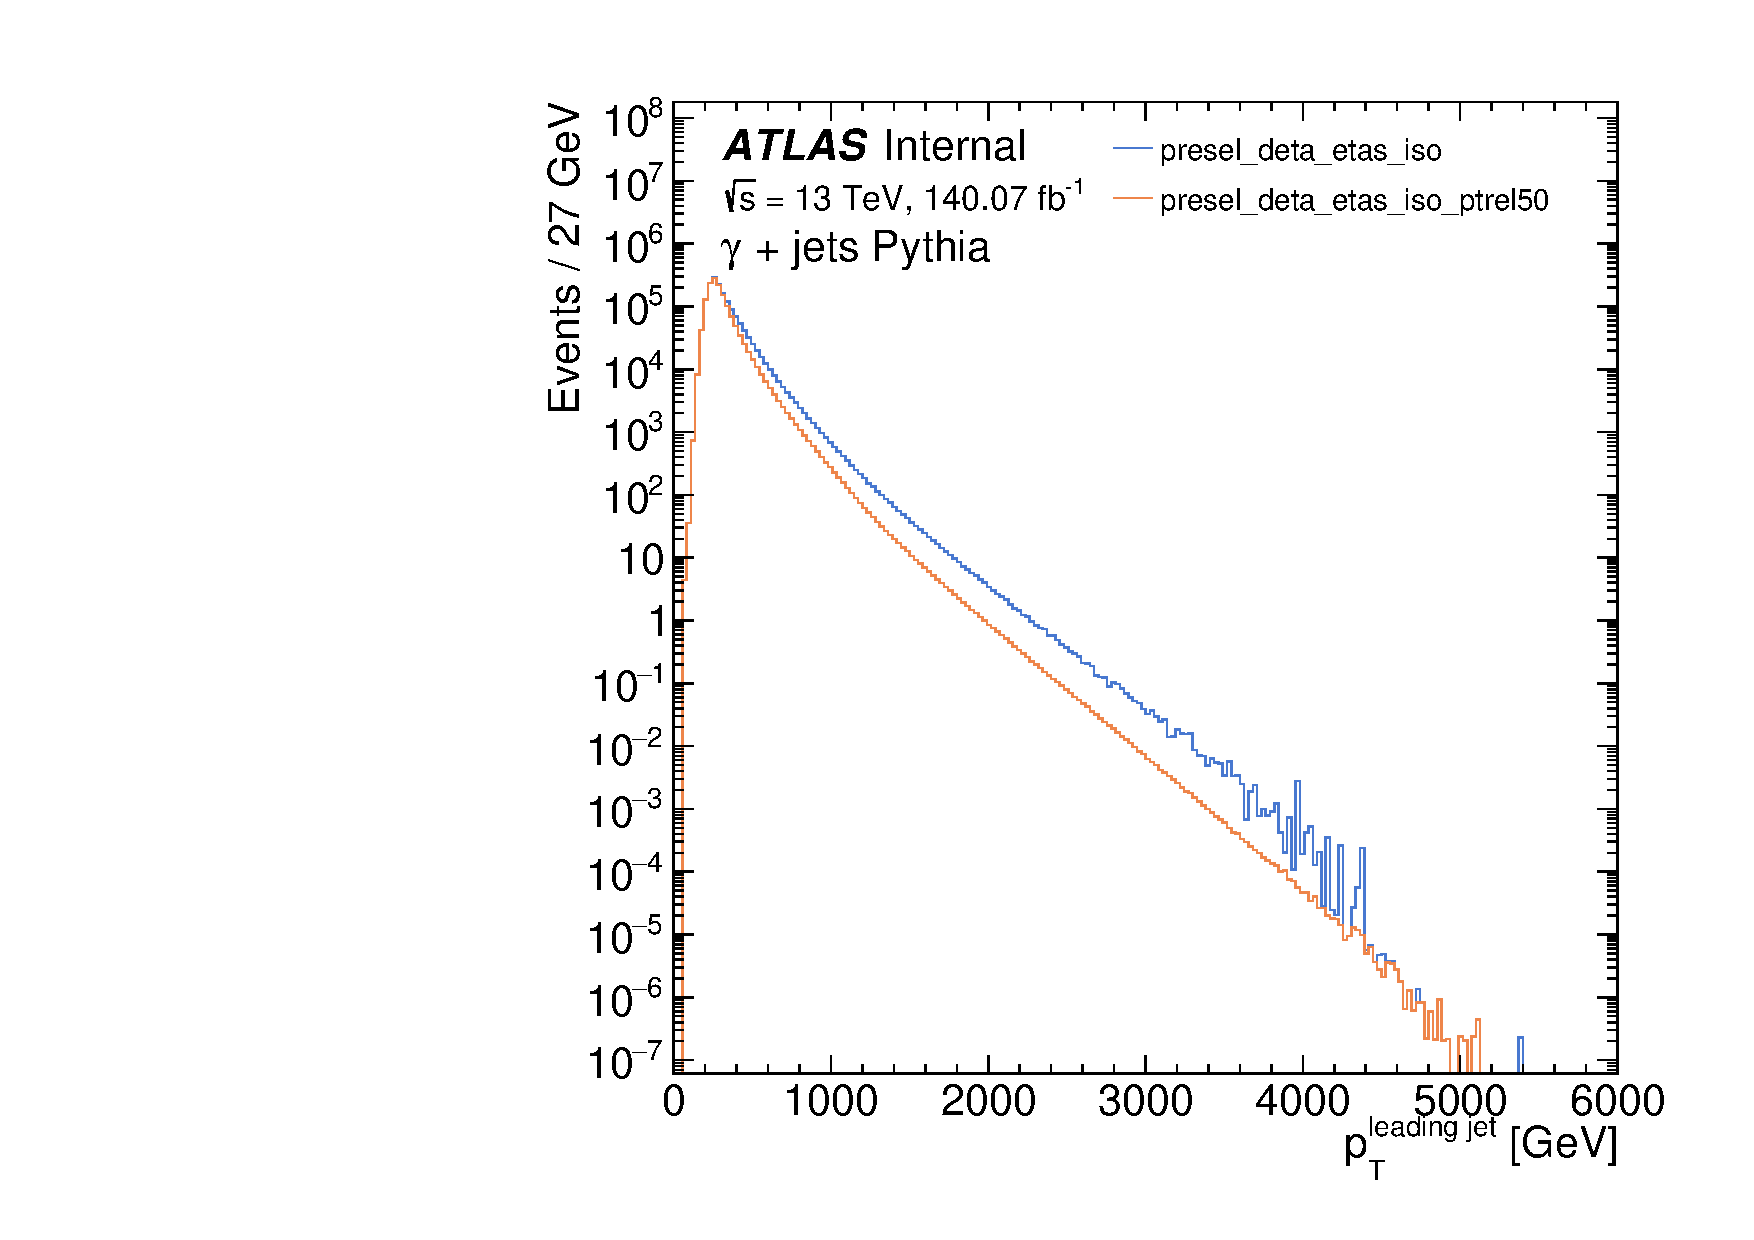
\includegraphics[width=\linewidth]{5_resonances/event_selection/jet_pt/can__photonjet_Pythia__jet_pt0__regions_presel_deta_etas_iso_presel_deta_etas_iso_ptrel50__Run2}
        \caption{Comparación final.}
    \end{subfigure}
    \caption{Distribución antes y después del corte en \ptjet para remover los eventos de \acp{FP}. Las contribuciones de \acp{DP} y de \acp{FP} se muestran por separado. En la figura de la derecha, la línea narnja (azul) representa la distribución luego (antes) de aplicar el corte en \ptjet.}
    \label{fig:evt_selection:sr_opt:jet_pt:jet_pt}
\end{figure}



\begin{figure}[ht!]
    \centering
    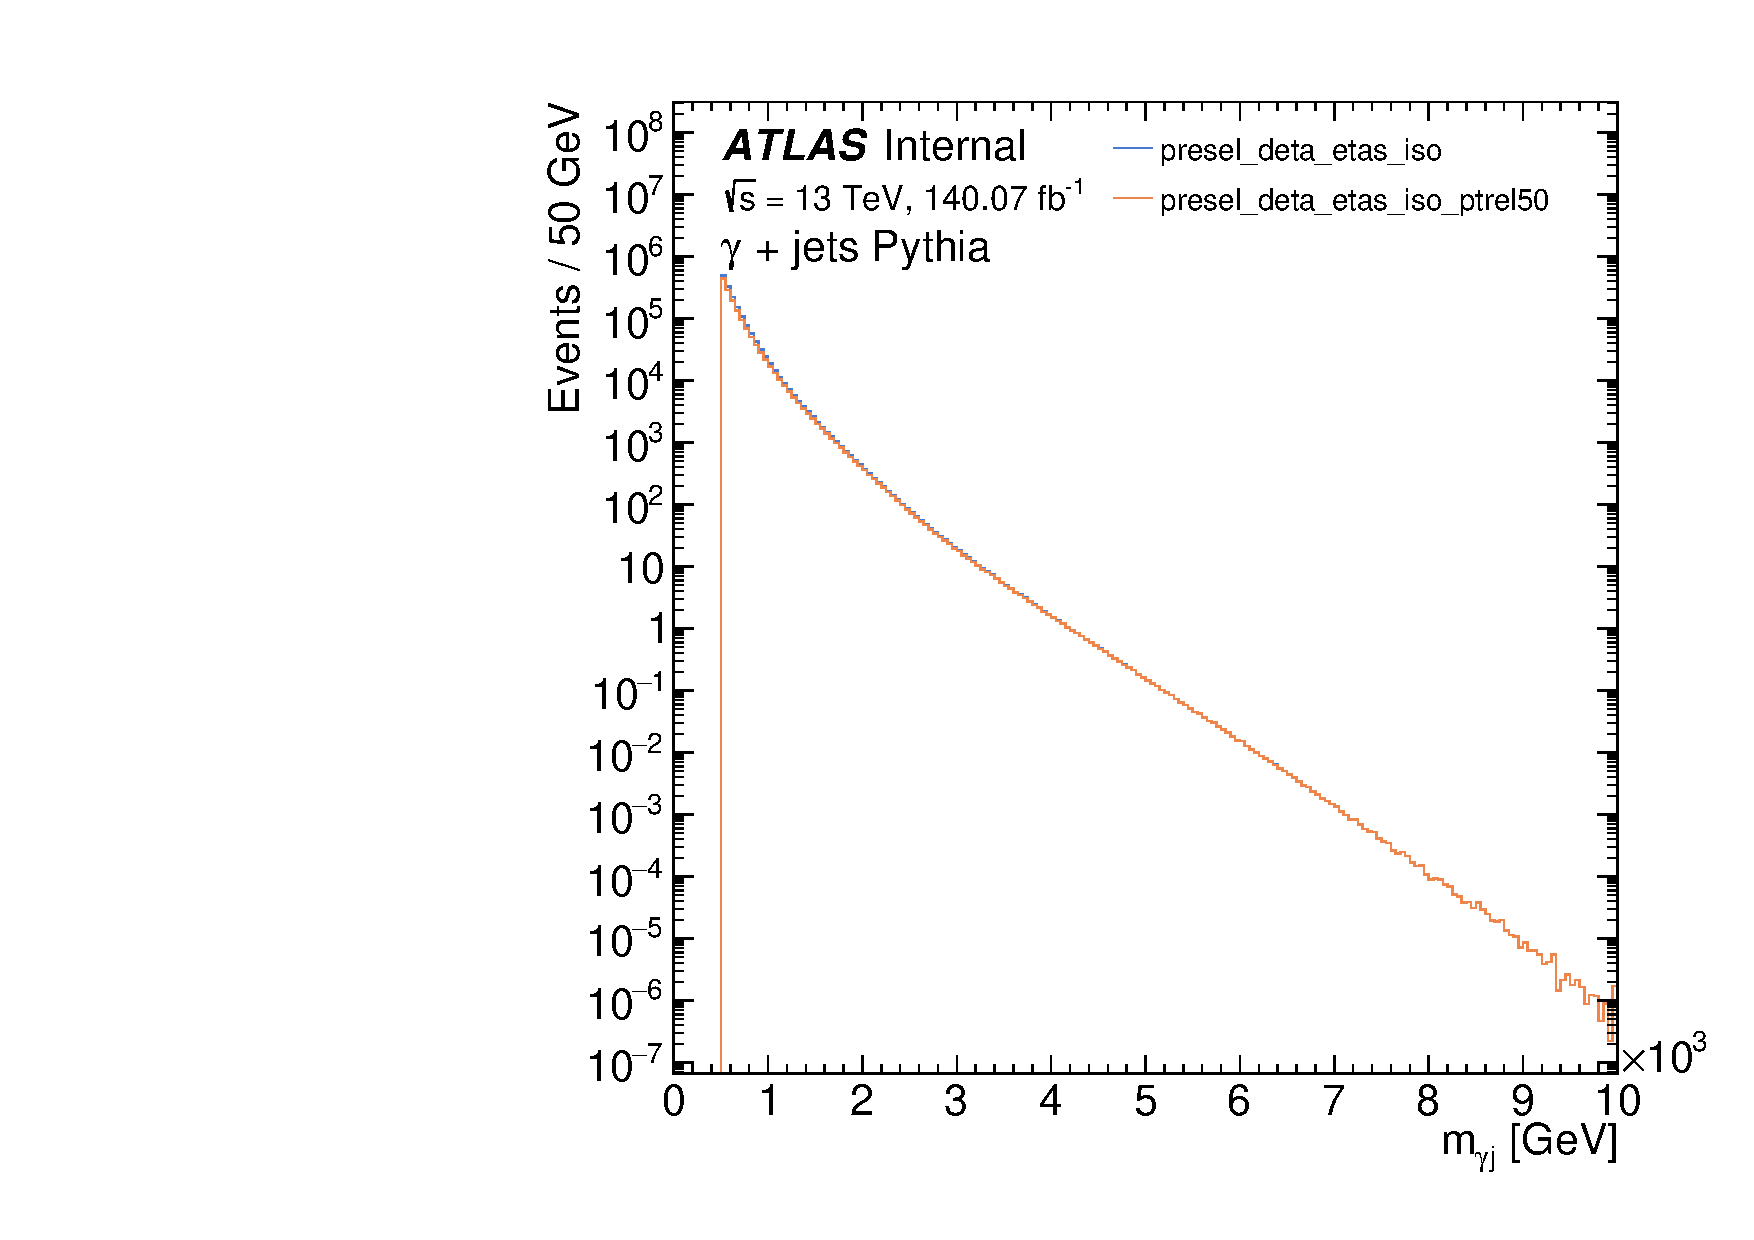
\includegraphics[width=0.45\linewidth]{5_resonances/event_selection/jet_pt/can__photonjet_Pythia__phjet_m__regions_presel_deta_etas_iso_presel_deta_etas_iso_ptrel50__Run2}
    \caption{Distribución de \myj antes y después del corte en \ptjet. La línea naranja (azul) representa la distribución antes (después) de la aplicación del corte.}
    \label{fig:evt_selection:sr_opt:jet_pt:phjet_m}
\end{figure}















\section{Regiones de señal}
\label{sec:evt_selection:sr}


Aplicando los cortes previamente definidos (resumidos en la \Tab{\ref{fig:evt_selection:sr:signal_regions_scheme}}) es posible obtener una distribución \myj limpia, en la que se eliminan la gran mayoría de \acp{FP} y eventos del canal \(t\) manteniendo una alta eficiencia de señal.

Para los objetivos de esta búsqueda, se clasifica al jet principal en tres posibles sabores: jets taggeados como light, \(c\) o \(b\). Haciendo uso del actual tagger de \ac{ATLAS} se pueden definir las regiones de señal SRB, SRC y SRL. En la \Fig{\ref{fig:evt_selection:sr:signal_regions_scheme}} se presenta un esquema de cómo se produce esta separación. En primer lugar, los \bjets se discriminan de light- y \cjets utilizando el \ac{WP} de \(77\%\) de eficiencia de \btagging. Al seleccionar aquellos jets que no consiguen entrar en la región SRB, se aplica el \ac{WP} de \ctagging de \(50\%\) de eficiencia para seleccionar \cjets y los que no pasan este \ctagger se clasifican como no etiquetados, o, simplemente \ljets.

\begin{table}[ht!]
    \caption{Definición de las regiones de señal.}
    \label{tab:evt_selection:sr:srs}
    \centering
    \begin{tabular}{|l|>{\centering\arraybackslash}p{0.08\linewidth}|>{\centering\arraybackslash}p{0.08\linewidth}|>{\centering\arraybackslash}p{0.08\linewidth}|>{\centering\arraybackslash}p{0.08\linewidth}|}
        \hline
        Cut                                     & SR & SRB & SRC & SRL \\
        \hline
        \ngamma                                 & \multicolumn{4}{c|}{$>0$} \\ \hline
        \ptgam [GeV]                            & \multicolumn{4}{c|}{$>150$} \\ \hline
        \njet                                   & \multicolumn{4}{c|}{$>0$} \\ \hline
        \ptjet [GeV]                            & \multicolumn{4}{c|}{$>150$} \\ \hline
        \etajet                                 & \multicolumn{4}{c|}{$<1.37 \,\,||\,\, (>1.52 \,\,\&\&\,\, <2.37)$} \\ \hline
        \myj [GeV]                              & \multicolumn{4}{c|}{$>500.$} \\ \hline
        \detayj                                 & \multicolumn{4}{c|}{$<1.6$} \\ \hline
        \etagam                                 & \multicolumn{4}{c|}{$<1.37$} \\ \hline
        \etajet                                 & \multicolumn{4}{c|}{$<1.37$} \\ \hline
        \(\Delta R_{\text{min}} (\gamma, j)\)   & \multicolumn{4}{c|}{$\geq 1.0$} \\ \hline
        \((\ptjet - \ptgam)/\ptgam\)            & \multicolumn{4}{c|}{$<0.5$} \\ \hline
        \btag \(77\%\)                          & - & Pasa   & \multicolumn{2}{c|}{Falla} \\ \hline
        \ctag \(50\%\)                          & - & -      & Pasa & Falla \\ \hline
    \end{tabular}
\end{table}

\begin{figure}[ht!]
    \centering
    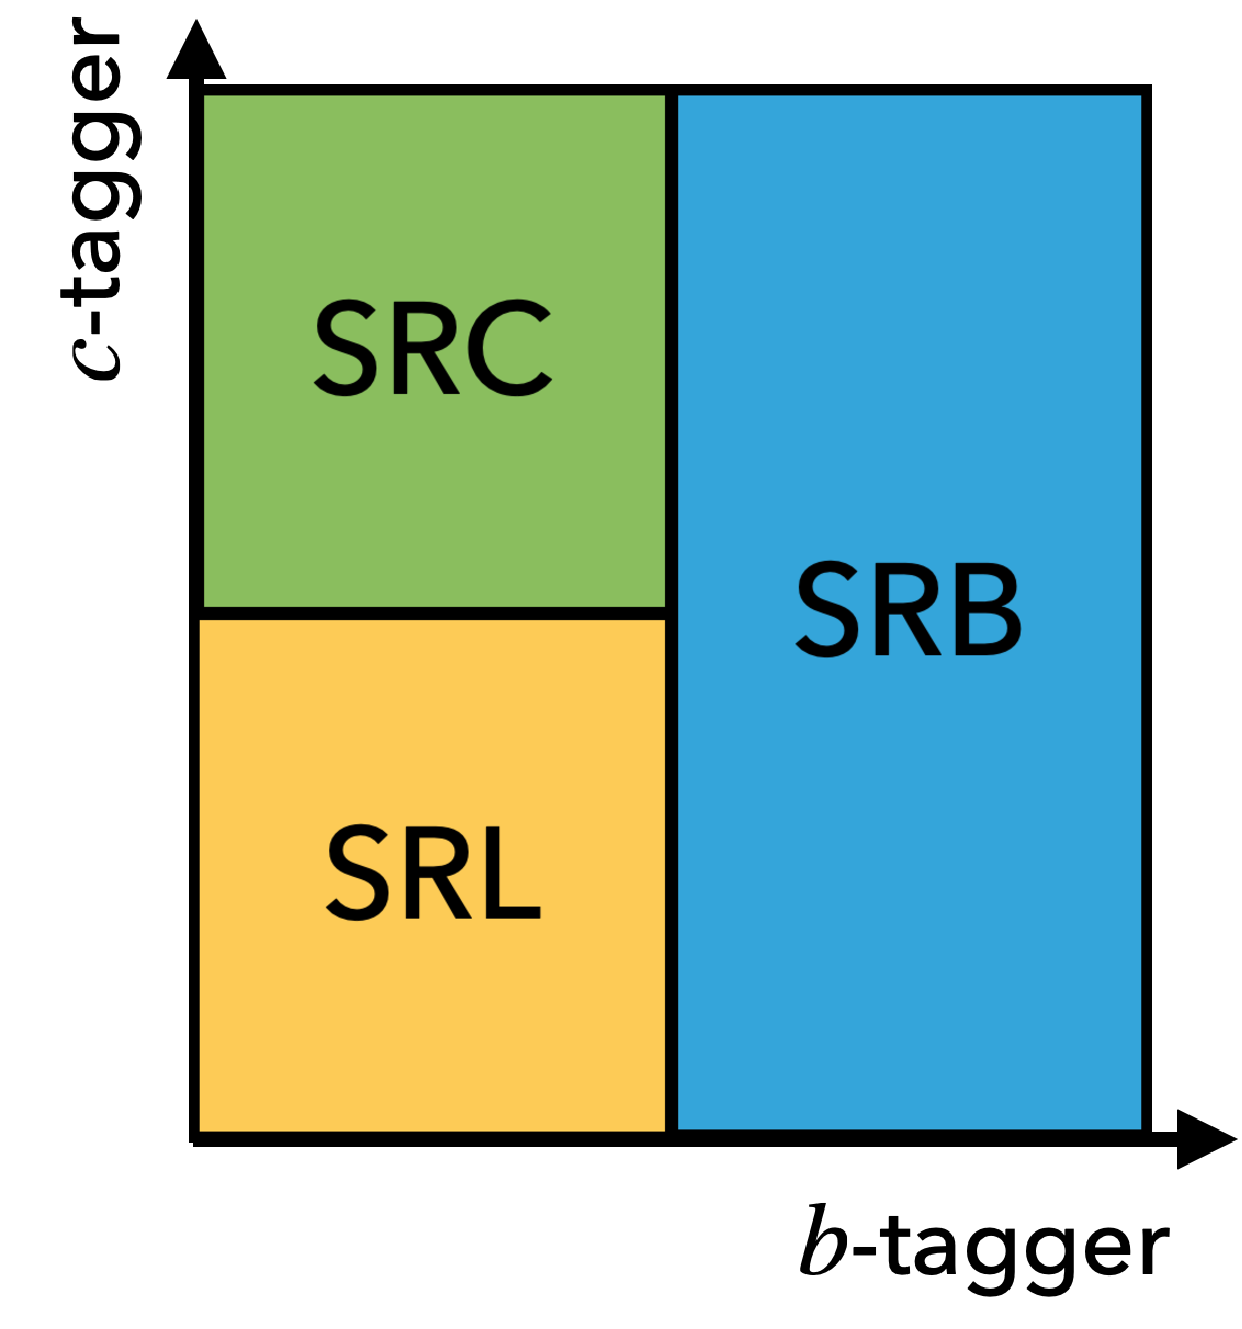
\includegraphics[width=0.35\linewidth]{5_resonances/event_selection/SRL_SRC_SRB-crop}
    \caption{Esquema del taggeo de jets bidimensional.}
    \label{fig:evt_selection:sr:signal_regions_scheme}
\end{figure}